\documentclass{report}
\usepackage[utf8]{inputenc}
\usepackage{amsmath}
\usepackage{geometry}
\geometry{
 a4paper,
 total={170mm,257mm},
 left=20mm,
 top=20mm,
 }
 \usepackage{siunitx}
 \usepackage{amsthm}
 \usepackage[utf8]{inputenc}
 \usepackage[italian]{babel}
\usepackage[T1]{fontenc}
\usepackage{amssymb}
\usepackage{physics}
\usepackage{commath}
\usepackage{tikz}
\usepackage{pgfplots}
\pgfplotsset{compat=1.15}
\usepackage{graphicx}
\graphicspath{ {Immagini/} }
\usepackage{float}
\usepackage{hyperref}
\hypersetup{
    colorlinks=true,
    linkcolor=red,
    citecolor=green
    filecolor=magenta,      
    urlcolor=cyan,
}
\usepackage{subcaption}
\usepackage{chngcntr}
\counterwithin*{equation}{section}

%Theorem Environments
\newtheorem{thm}{Teorema}[section]
\newtheorem{lem}[thm]{Lemma}
\newtheorem{property}{Proprietà}[section]
\newtheorem{defn}{Definizione}[section]
\newtheorem{prop}[defn]{Proposizione}
\newtheorem{example}{Esempi}[subsection]
\newtheorem{exerc}[example]{Esercizi Svolti}
\newtheorem{enunc}[defn]{Enunciato}

%Commandi di Formattazione
\newcommand{\noi}{\noindent}
\newcommand{\note}{\noindent {\quad \bf \underline{Osservazione:}} \quad}
\newcommand{\eg}{\noindent {\bf \underline{Esempio:}} \quad}
\newcommand{\bfemph}[1]{\textbf{\textit{#1}}}
\renewcommand{\emph}[1]{\bfemph{#1}}

%Number Sets
\newcommand{\R}{\mathbb{R}}
\newcommand{\C}{\mathbb{C}}
\newcommand{\Z}{\mathbb{Z}}
\newcommand{\Q}{\mathbb{Q}}

%Shortcuts
\newcommand{\then}{\ensuremath{\Rightarrow}}
\newcommand{\twopartdef}[4]
{
	\left\{
		\begin{array}{ll}
			#1 & \mbox{se } #2 \\
			#3 & \mbox{se } #4
		\end{array}
	\right.
}

%Vectors
\renewcommand{\i}{\vu{i}}
\renewcommand{\j}{\vu{j}}
\renewcommand{\k}{\vu{k}}
\renewcommand{\a}{\va{a}}
\renewcommand{\b}{\va{b}}
\renewcommand{\c}{\va{c}}
\renewcommand{\v}{\va{v}}
\renewcommand{\u}{\va{u}}
\newcommand{\s}{\va{s}}
\renewcommand{\t}{\va{t}}
\newcommand{\verst}{\vu{t}}
\newcommand{\versr}{\vu{r}}
\renewcommand{\r}{\va{r}}
\newcommand{\tauvs}{\vu{\tau}}
\newcommand{\tauvt}{\va{\tau}}
\newcommand{\normvs}{\vu{n}}
\newcommand{\N}{\va{N}}
\newcommand{\g}{\va{g}}
\newcommand{\F}{\va{F}}
\newcommand{\f}{\va{f}}
\newcommand{\M}{\va{M}}
\renewcommand{\l}{\va{l}}
\newcommand{\p}{\va{p}}
\renewcommand{\P}{\va{P}}
\renewcommand{\L}{\va{L}}
\newcommand{\A}{\va{A}}
\newcommand{\I}{\va{I}}



\renewcommand{\c}{\overline{c}}
\title{Meccanica e Termodinamica}
\author{Roberto Gargiulo}
\date{Ultimo Aggiornamento: \today}


\begin{document}

\maketitle
\tableofcontents

\part{Meccanica}
\chapter{Cinematica del Corpo Puntiforme}
\section{Introduzione}
La cinematica del corpo puntiforme è la parte della meccanica che si occupa di descrivere il moto di un corpo. Si parla di \textbf{moto} quando un corpo cambia la propria posizione nel tempo rispetto ad un riferimento. L'insieme delle posizioni di un corpo costituisce la sua \textbf{traiettoria}. Quando la traiettoria di un corpo appartiene a un piano, i due sistemi di riferimento più comodi sono due: un sistema di \textbf{coordinate polari} oppure un sistema di \textbf{coordinate cartesiane}.
\paragraph{Coordinate Polari}
Le coordinate polari sono un sistema di coordinate in cui ogni punto è determinato unicamente dalla distanza da un punto detto \textbf{polo} e dall'angolo formato dalla semiretta congiungente il polo e il punto (considerato positivo in senso antiorario) e la semiretta uscente dal polo detta \textbf{asse polare}.
\begin{figure}[H]
    \centering
    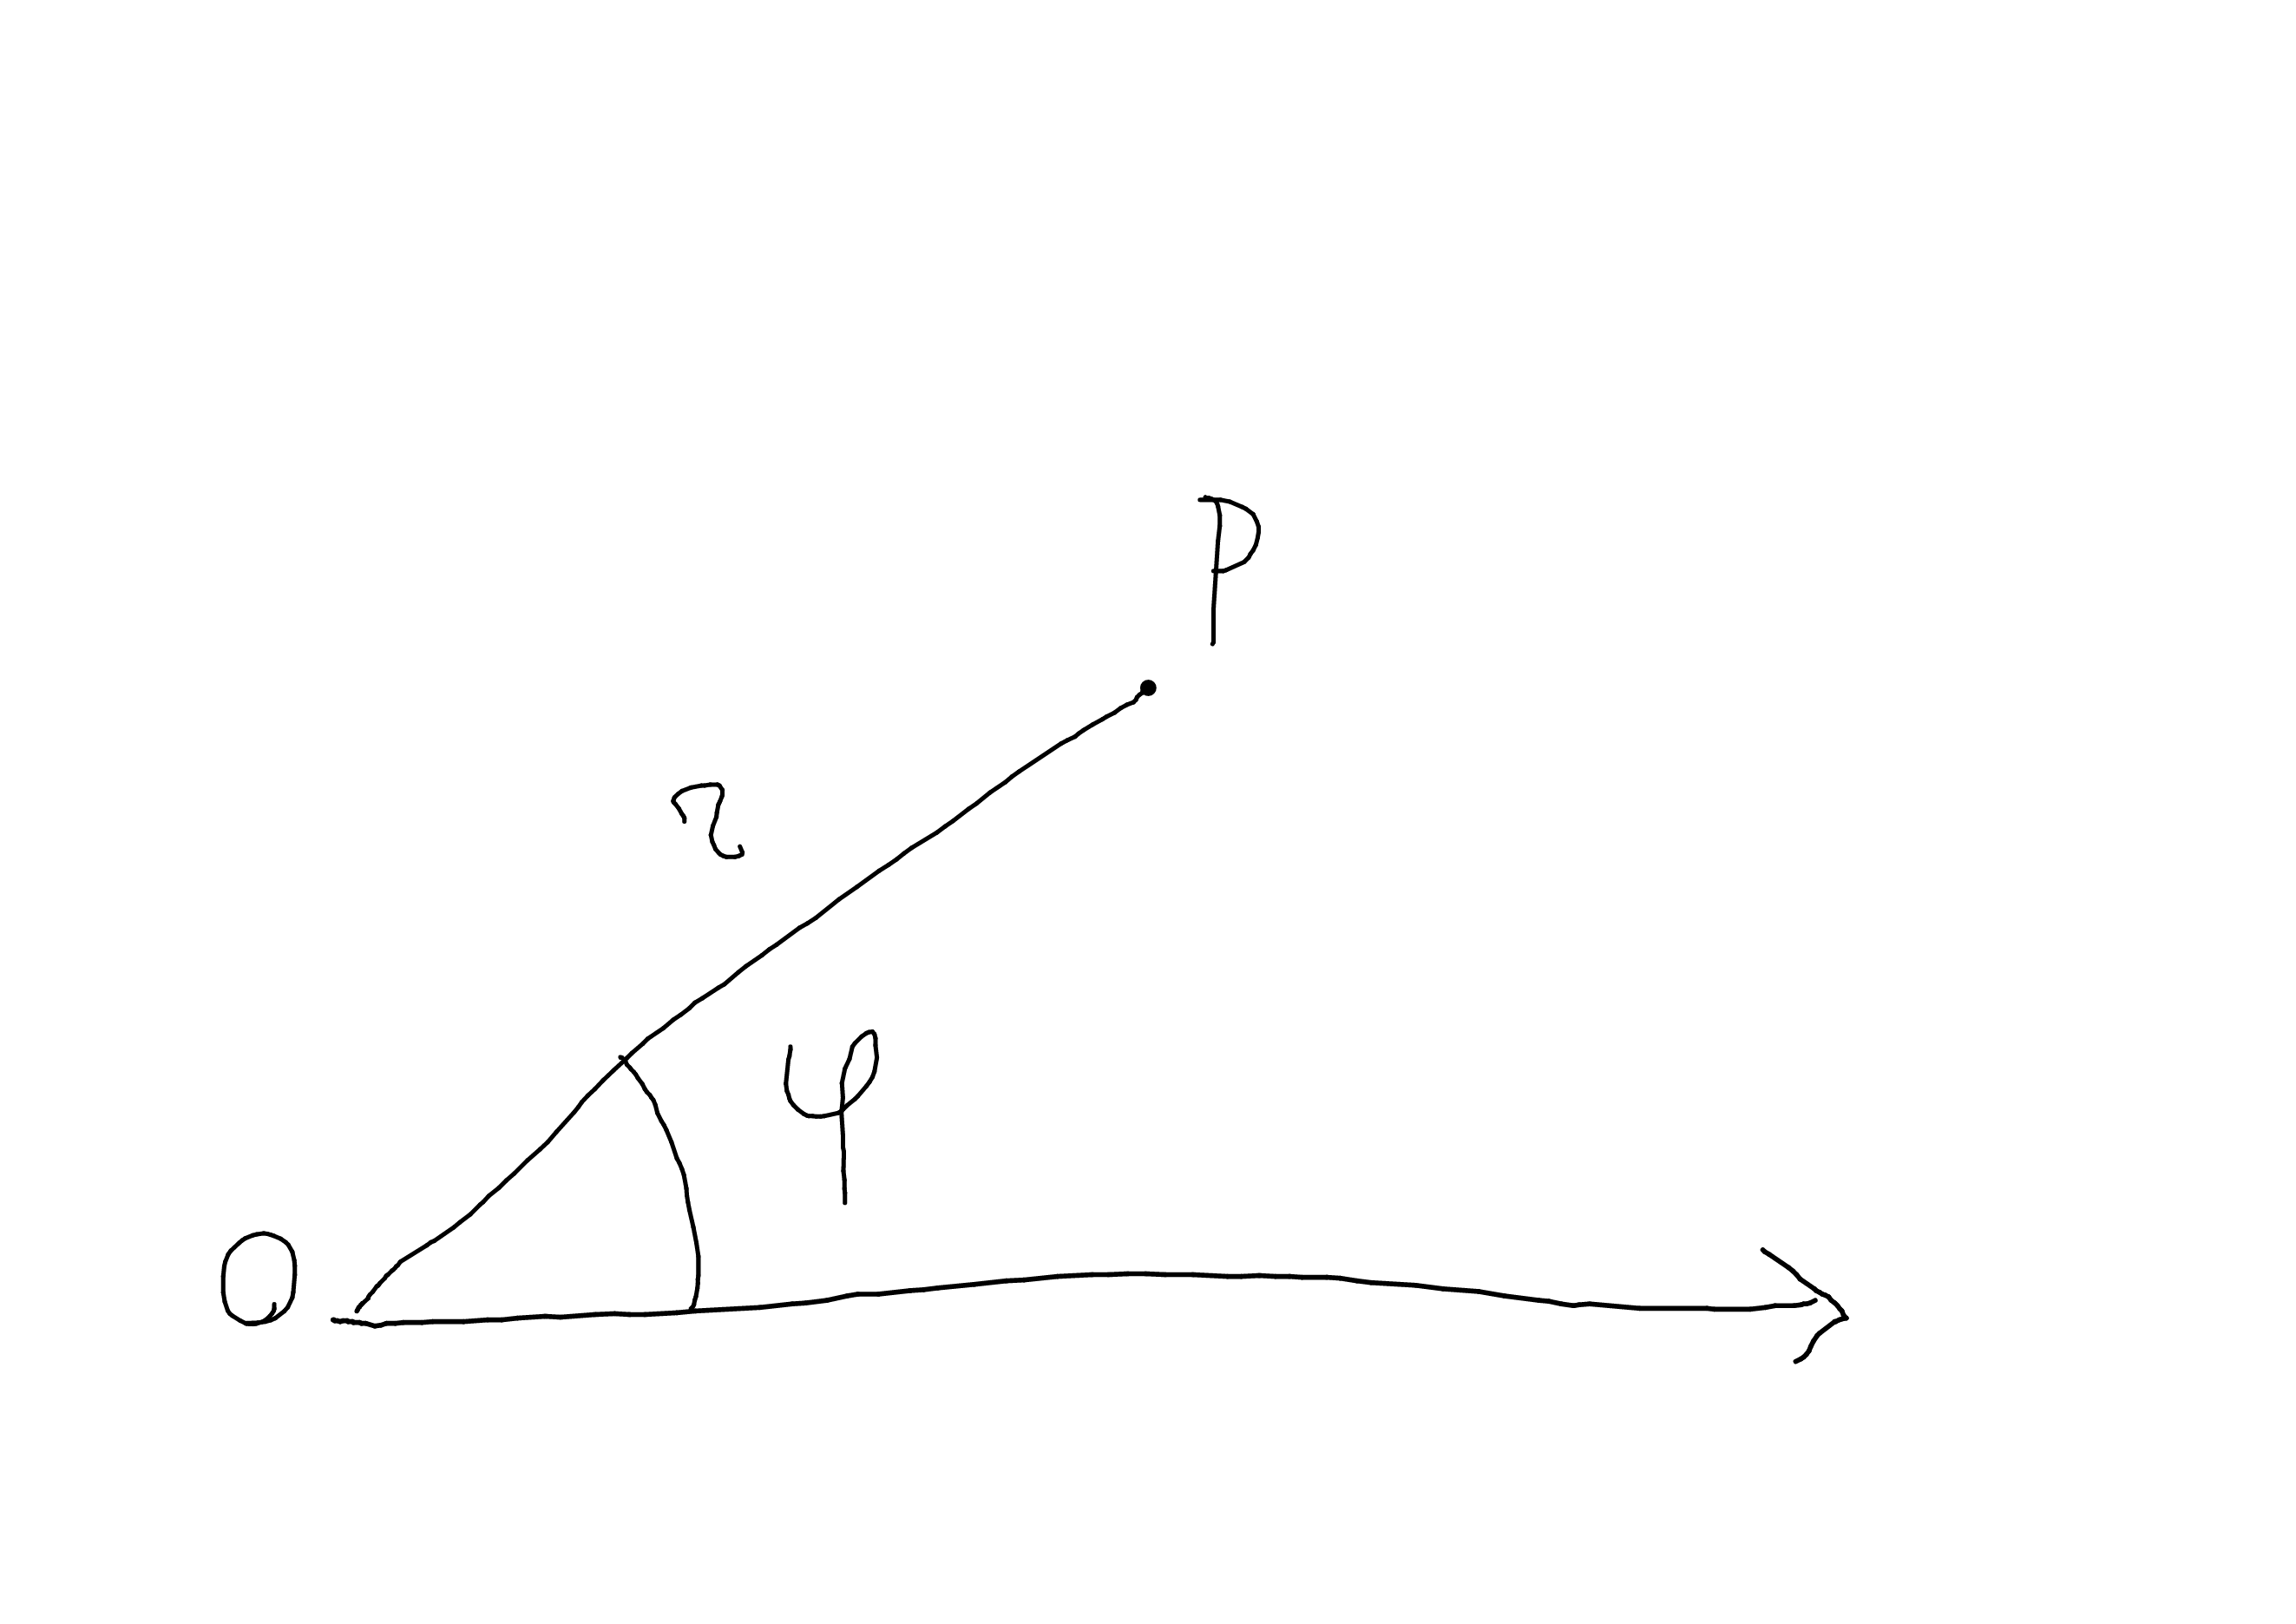
\includegraphics[width=0.5\textwidth]{CoordPolari.png}
\end{figure}
\paragraph{Coordinate Cartesiane}
Il sistema di assi cartesiani è invece determinato dalla distanza del punto da assi perpendicolari (\textbf{cartesiani}) passanti per un punto detto \textbf{origine}.
\begin{figure}[H]
    \centering
    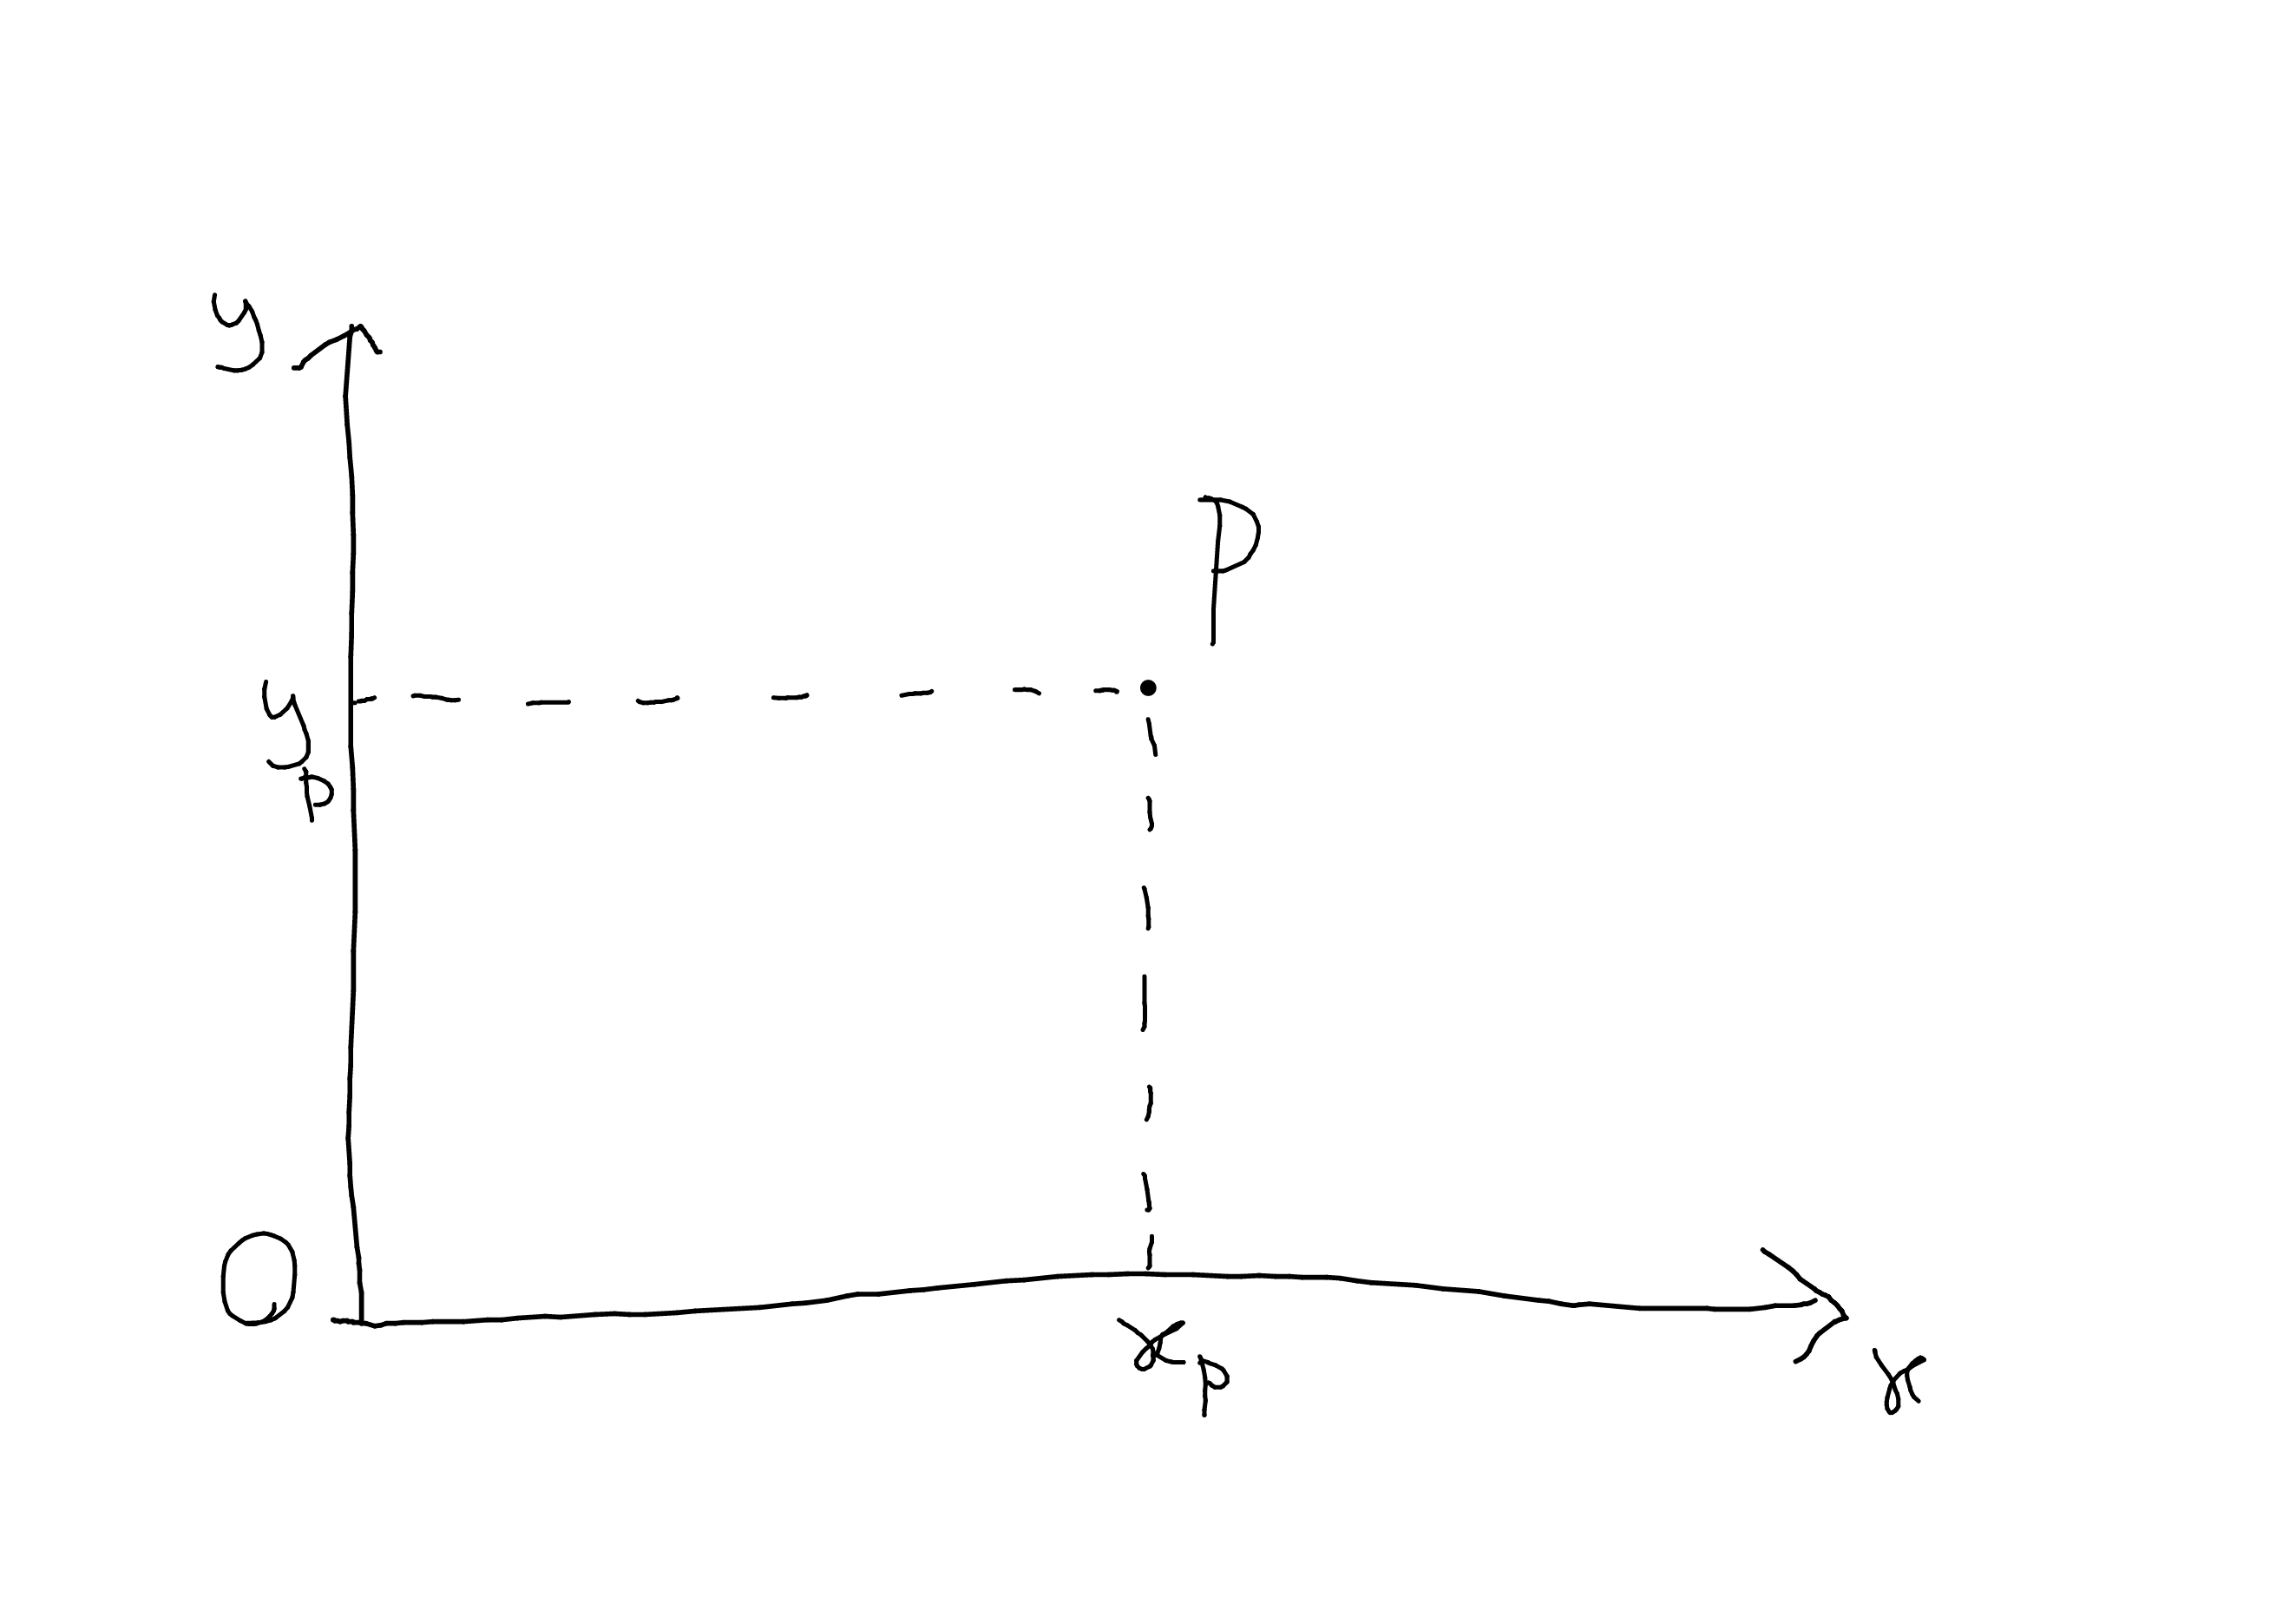
\includegraphics[width=0.5\textwidth]{CoordCartesiane.png}
\end{figure}

\paragraph{Formule di Cambiamento di Riferimento}
Per cambiare sistema di riferimento (lasciando fissa l'origine/polo) da un sistema cartesiano a uno polare e viceversa si possono ricavare le seguenti formule:
\begin{equation}
\begin{cases}
x=r\cos\phi\\
y=r\sin\phi
\end{cases}\iff
\begin{cases}
\tan\phi=\frac{y}{x}\\
r=\sqrt{x^y+y^2}
\end{cases}
\end{equation}
Altre formule per il cambiamento di riferimento sono quelle per la \textbf{traslazione} e \textbf{rotazione} di un sistema cartesiano:
\begin{equation}
\begin{cases}
x'=x+u\\
y'=y+v
\end{cases}\quad
\begin{pmatrix}
x'\\y'
\end{pmatrix}=
\begin{pmatrix}
\cos\theta&-\sin\theta\\
\sin\theta&\cos\theta
\end{pmatrix}
\begin{pmatrix}
x\\y
\end{pmatrix}
\end{equation}
\paragraph{Cenni sui Vettori}
Di particolare importanza sui vettori sono le seguenti operazioni e teoremi:
\begin{enumerate}
    \item Prodotto Scalare
    \item Prodotto Vettoriale
    \item Teorema di Carnot
\end{enumerate}
\paragraph{Il Punto Materiale}
Elemento centrale in meccanica è l'idea di \textbf{punto materiale} (o corpo puntiforme), ossia un corpo le cui dimensioni sono tanto piccole rispetto al sistema in cui viene considerato da essere trascurabili. In questo modo un corpo puntiforme è un oggetto che si può studiare facilmente in un sistema di coordinate cartesiane/polari e sono ben definiti i vettori posizione e spostamento.\\
Per affrontare la cinematica risulta necessario enunciare il \textbf{primo principio della dinamica}, che afferma:
\begin{enunc}
Un corpo mantiene il suo stato di moto rettilineo uniforme o di quiete se la risultante delle forze agenti su di esso è nulla. 
\end{enunc}
Studiamo più in dettaglio come descrivere il moto di un corpo puntiforme.
\section{Velocità e Accelerazione}
Noto il concetto di \textbf{vettore posizione} $\r$ come quel vettore che parte dall'origine e punta verso il punto materiale di posizione P, ha senso definire \textit{come} questo vettore varia nel tempo, calcolandone la velocità come lo spazio percorso rispetto al tempo necessario a percorrerlo. Questo vettore è detto \textbf{velocità media}:
\[\v_m=\frac{\Delta \r}{\Delta t}\]
Per ottenere un vettore capace di descrivere il moto di un corpo istante per istante, dobbiamo calcolare invece la derivata temporale, ottenendo quindi la \textbf{velocità istantanea}:
\[\v=\dv{\r}{t}\]
Similmente possiamo introdurre la grandezza \textbf{accelerazione} media e istantanea come misura della variazione della velocità nel tempo:
\[\a_m=\frac{\Delta v}{\Delta t}\quad\a=\dv{\v}{t}\]
Notiamo che la derivata di un vettore è perpendicolare al vettore stesso, utilizzando la proprietà della derivata rispetto al prodotto vettoriale
\begin{align*}
    \r\cdot\r=|\r|^2\\
    \dv{\r\cdot\r}{t}=\dv{|\r^2|}{t}=0\\
    \dv{\r}{t}\cdot\r+\r\cdot\dv{\r}{t}=0\\
    2\r\cdot\dv{\r}{t}=0\iff\r\perp\dv{\r}{t}
\end{align*}
\subsection{Ascissa Curvilinea}
Per studiare i moti piani è particolarmente utile introdurre il concetto di \textbf{ascissa curvilinea}, una ri-parametrizzazione della curva tracciata dal corpo in moto, fissando un punto e ottenendo la distanza da tale lungo la curva. Otteniamo in questo modo la possibilità di descrivere la distanza percorsa lungo una curva come segue:
\[\dif s=\pm\sqrt{(\dif x)^2+(\dif y)^2}=|\dif\r|\then s(t)=\int_0^t\dif s\]
Da questa proprietà ricaviamo che il modulo della velocità di un corpo può essere scritto come la derivata temporale dell'ascissa curvilinea:
\[|\v(t)|=\abs{\dv{\r}{t}}=\abs{\dv{s}{t}}=\abs{v_s}\]
La velocità può essere scritta dunque come il prodotto tra la derivata dell'ascissa curvilinea (la \textbf{velocità scalare}) e il versore tangente:
\[\v(t)=v_s(t)\va{\tau}(t)\]
Similmente possiamo ottenere un risultato rispetto all'accelerazione derivando ancora una volta:
\begin{equation}
\begin{split}
  \a(t)&=\dv{\v(t)}{t}=\dv{v_s\va{\tau}}{t}=\\
  &=\dv{v_s}{t}\va{\tau}+v_s\dv{\va{\tau}}{t}=\\
  &=a_s\va{\tau}-\dv{s}{t}\dv{\phi}{t}\va{n}=\\
  &=a_s\va{\tau}-\dv{s}{t}\dv{\phi}{s}\dv{s}{t}\va{n}=\\
  &=a_s\va{\tau}-\dv{\phi}{s}\left(\dv{s}{t}\right)^2\va{n}=\\
  &=a_s\va{\tau}-\frac{1}{R(t)}v_s^2\va{n}=\\
  &=\boxed{a_s\va{\tau}-\frac{v^2}{R}\va{n}=\a_{\tau}+\a_{\va{n}}}
\end{split}
\end{equation}
Ossia utilizzando l'ascissa curvilinea possiamo esprimere l'accelerazione in una componente tangenziale ed una "normale" che prendono il nome rispettivamente di \textbf{accelerazione tangenziale} e \textbf{accelerazione centripeta}. Questa componente è detta centripeta in quanto (come fatto notare al penultimo passaggio) essa punta istantaneamente verso il centro di una circonferenza, detta \textbf{circonferenza osculatrice}, capace di approssimare la curva in quell'intorno.\\
Il centro di questa circonferenza è detto \textbf{centro di curvatura} e il suo raggio è invece \textbf{raggio di curvatura}: maggiore è il raggio di curvatura, minore l'accelerazione centripeta, in quanto significa che la circonferenza tende sempre più ad una retta, risultando "meno curva".
\begin{figure}[H]
    \centering
    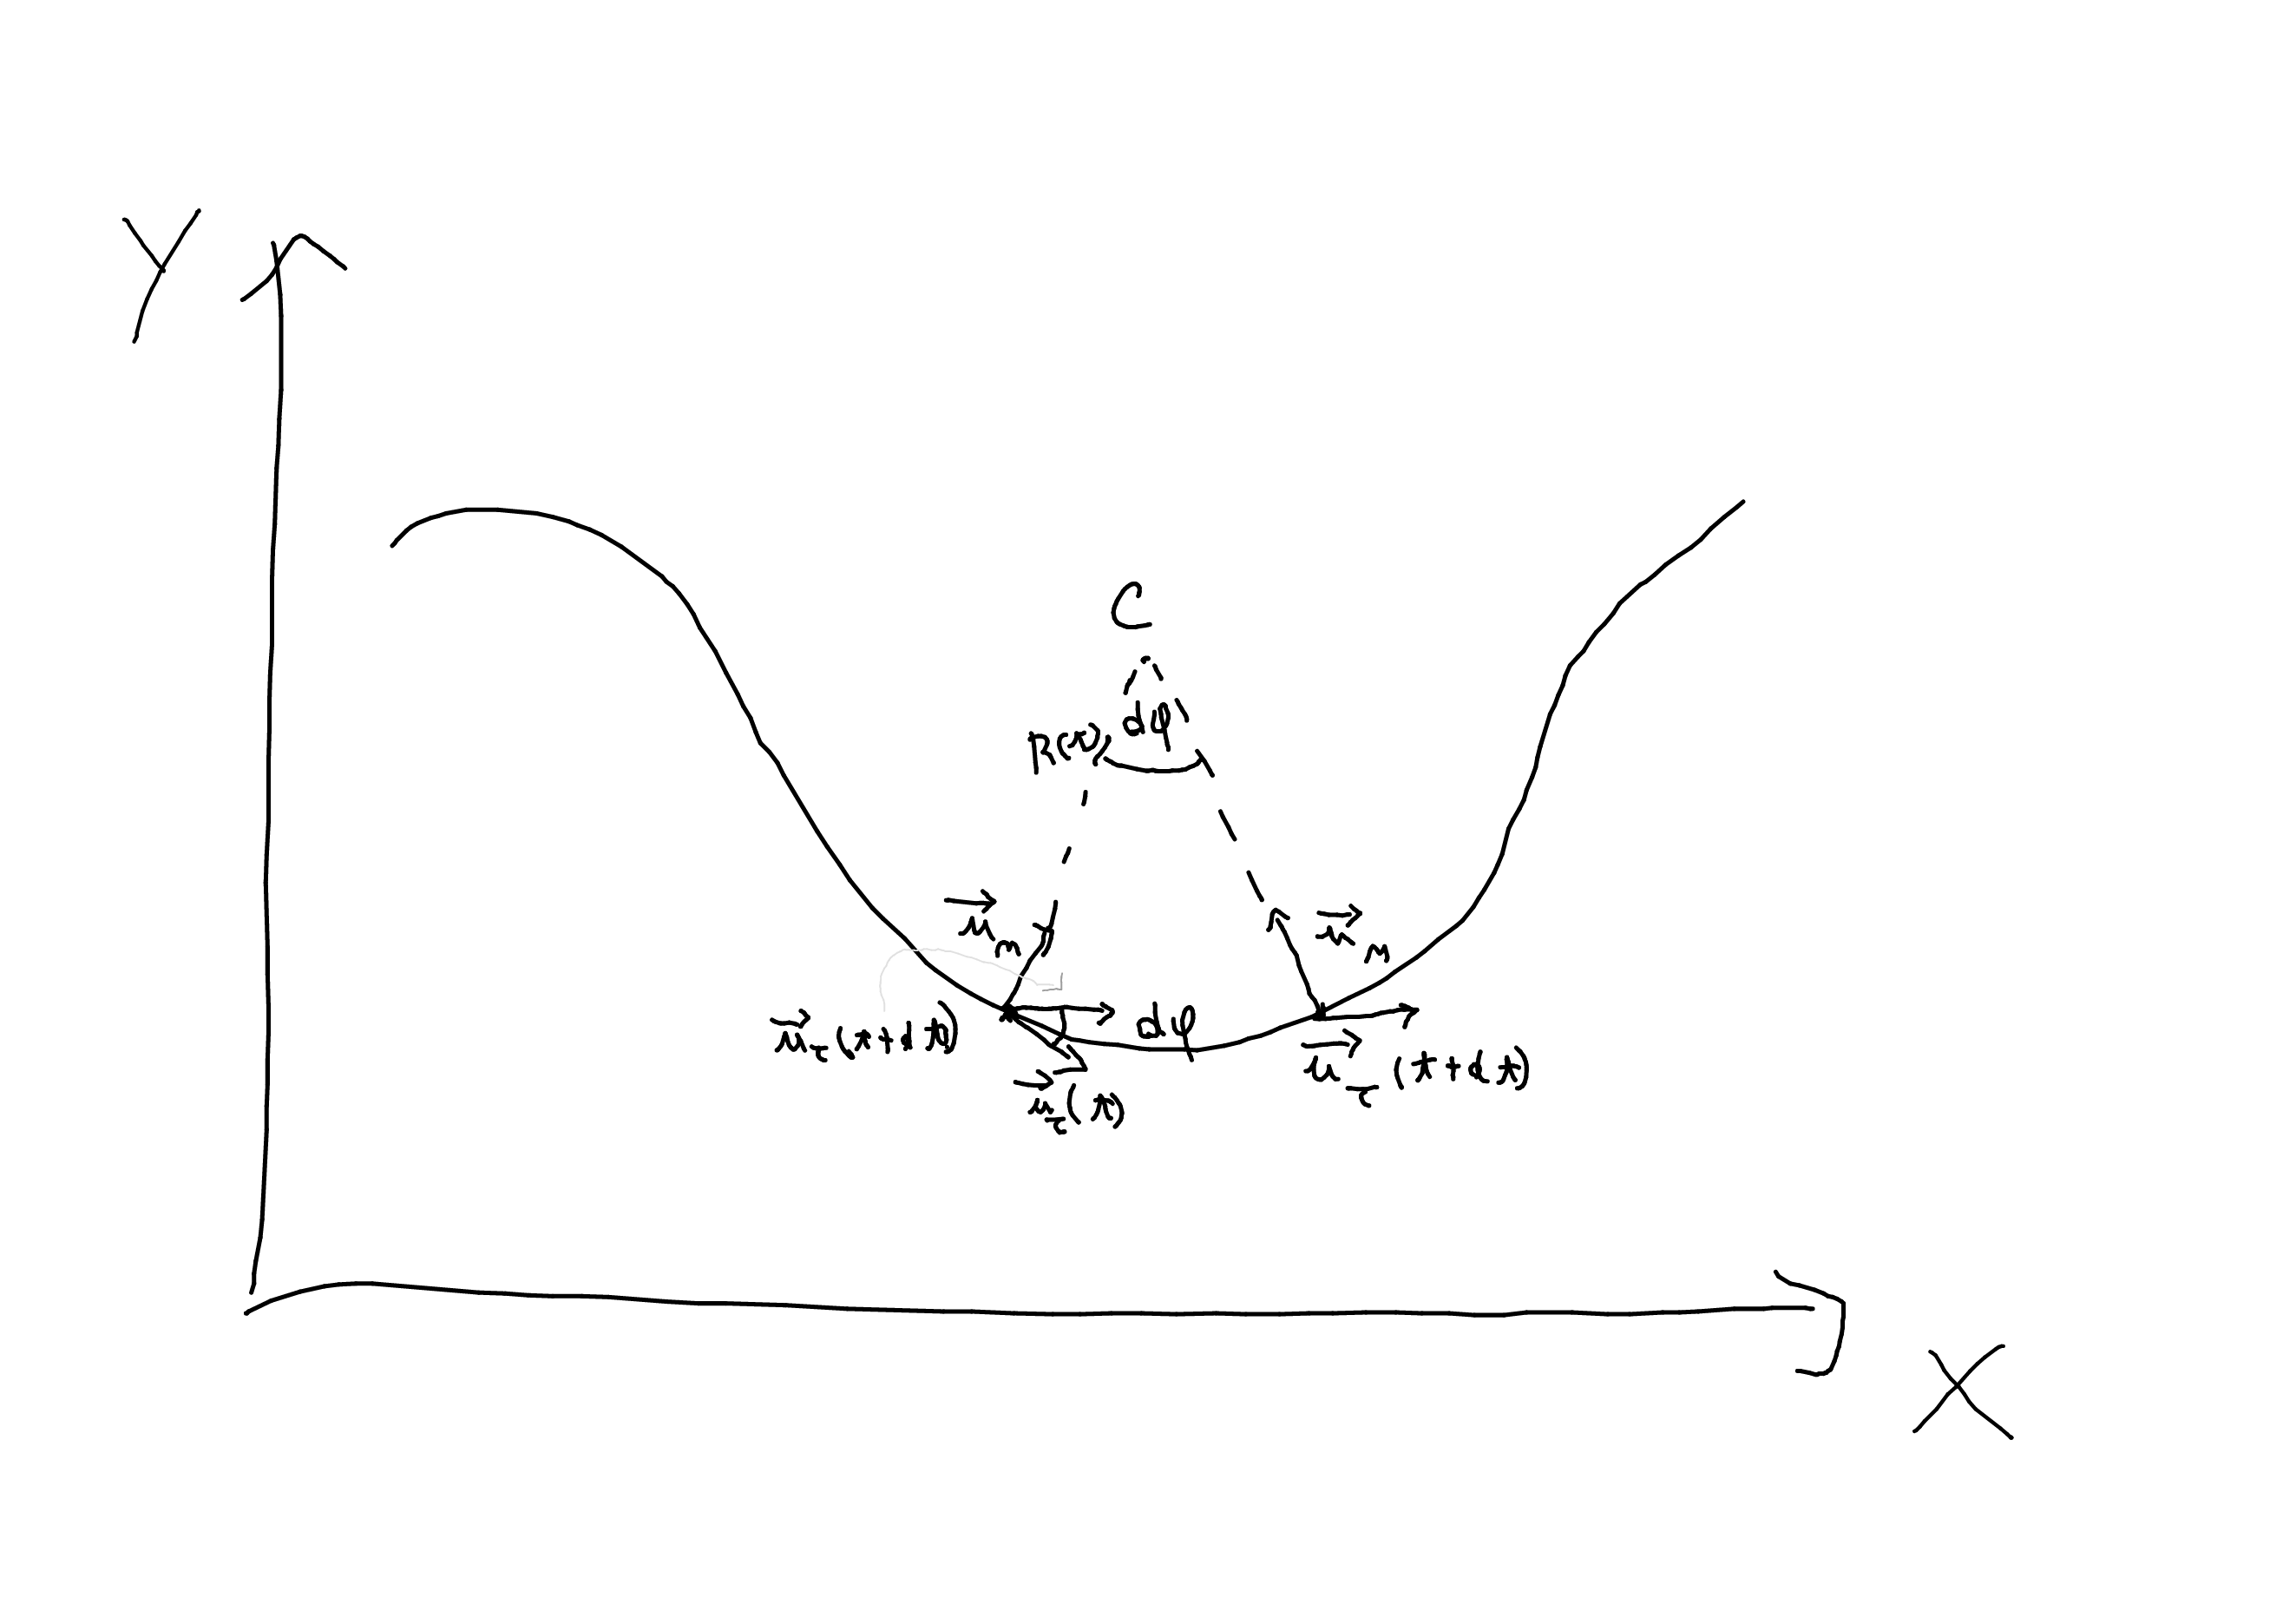
\includegraphics[width=0.5\textwidth]{CircOscul.png}
\end{figure}
\subsection{Componenti Polari della Velocità}
Detto $\u_{\r}$ il versore radiale (parallelo ad $\r$) e $\u_{\theta}$ il versore ad esso perpendicolare, possiamo scrivere la velocità come segue utilizzando le proprietà della derivata ed esprimendo il \textbf{raggio vettore} come $\r=r\u_{\r}$:
\[\v=\dv{\r}{t}=\dv{r\u_{\r}}{t}=\dv{r}{t}\u_{\r}+r\dv{\u_{\r}}{t}=\boxed{\dv{r}{t}\u_{\r}+r\dv{\theta}{t}\u_{\theta}=\v_{\r}+\v_{\theta}}\]
\begin{figure}[H]
    \centering
    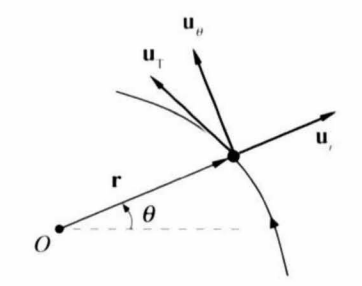
\includegraphics[width=0.3\textwidth]{ComponentiPolariVelocit.png}
\end{figure}
\begin{figure}[H]
    \centering
    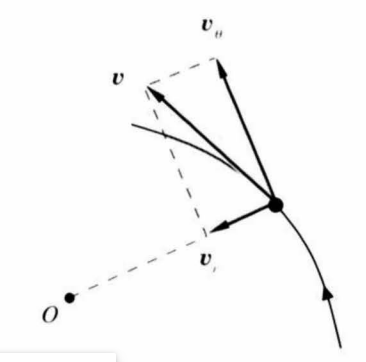
\includegraphics[width=0.3\textwidth]{CompPolVel.png}
\end{figure}
\subsection{Il Vettore Ruotante}
Si definisce \textbf{vettore ruotante} un vettore che mantiene il proprio modulo costante, pur cambiando direzione. Ha particolare rilevanza studiare il comportamento di un vettore ruotante e della sua derivata per studiare i moti circolari.
\paragraph{Derivata di un Vettore Ruotante}
Consideriamo per comodità il caso di un vettore $\va{A}$ che ruota in senso antiorario (in modo che l'angolo spazziato sia positivo). I vettori $\va{A(t)},\va{A(t+\Delta t)},\Delta \va{A}$ determinano un triangolo isoscele:
\begin{figure}[H]
    \centering
    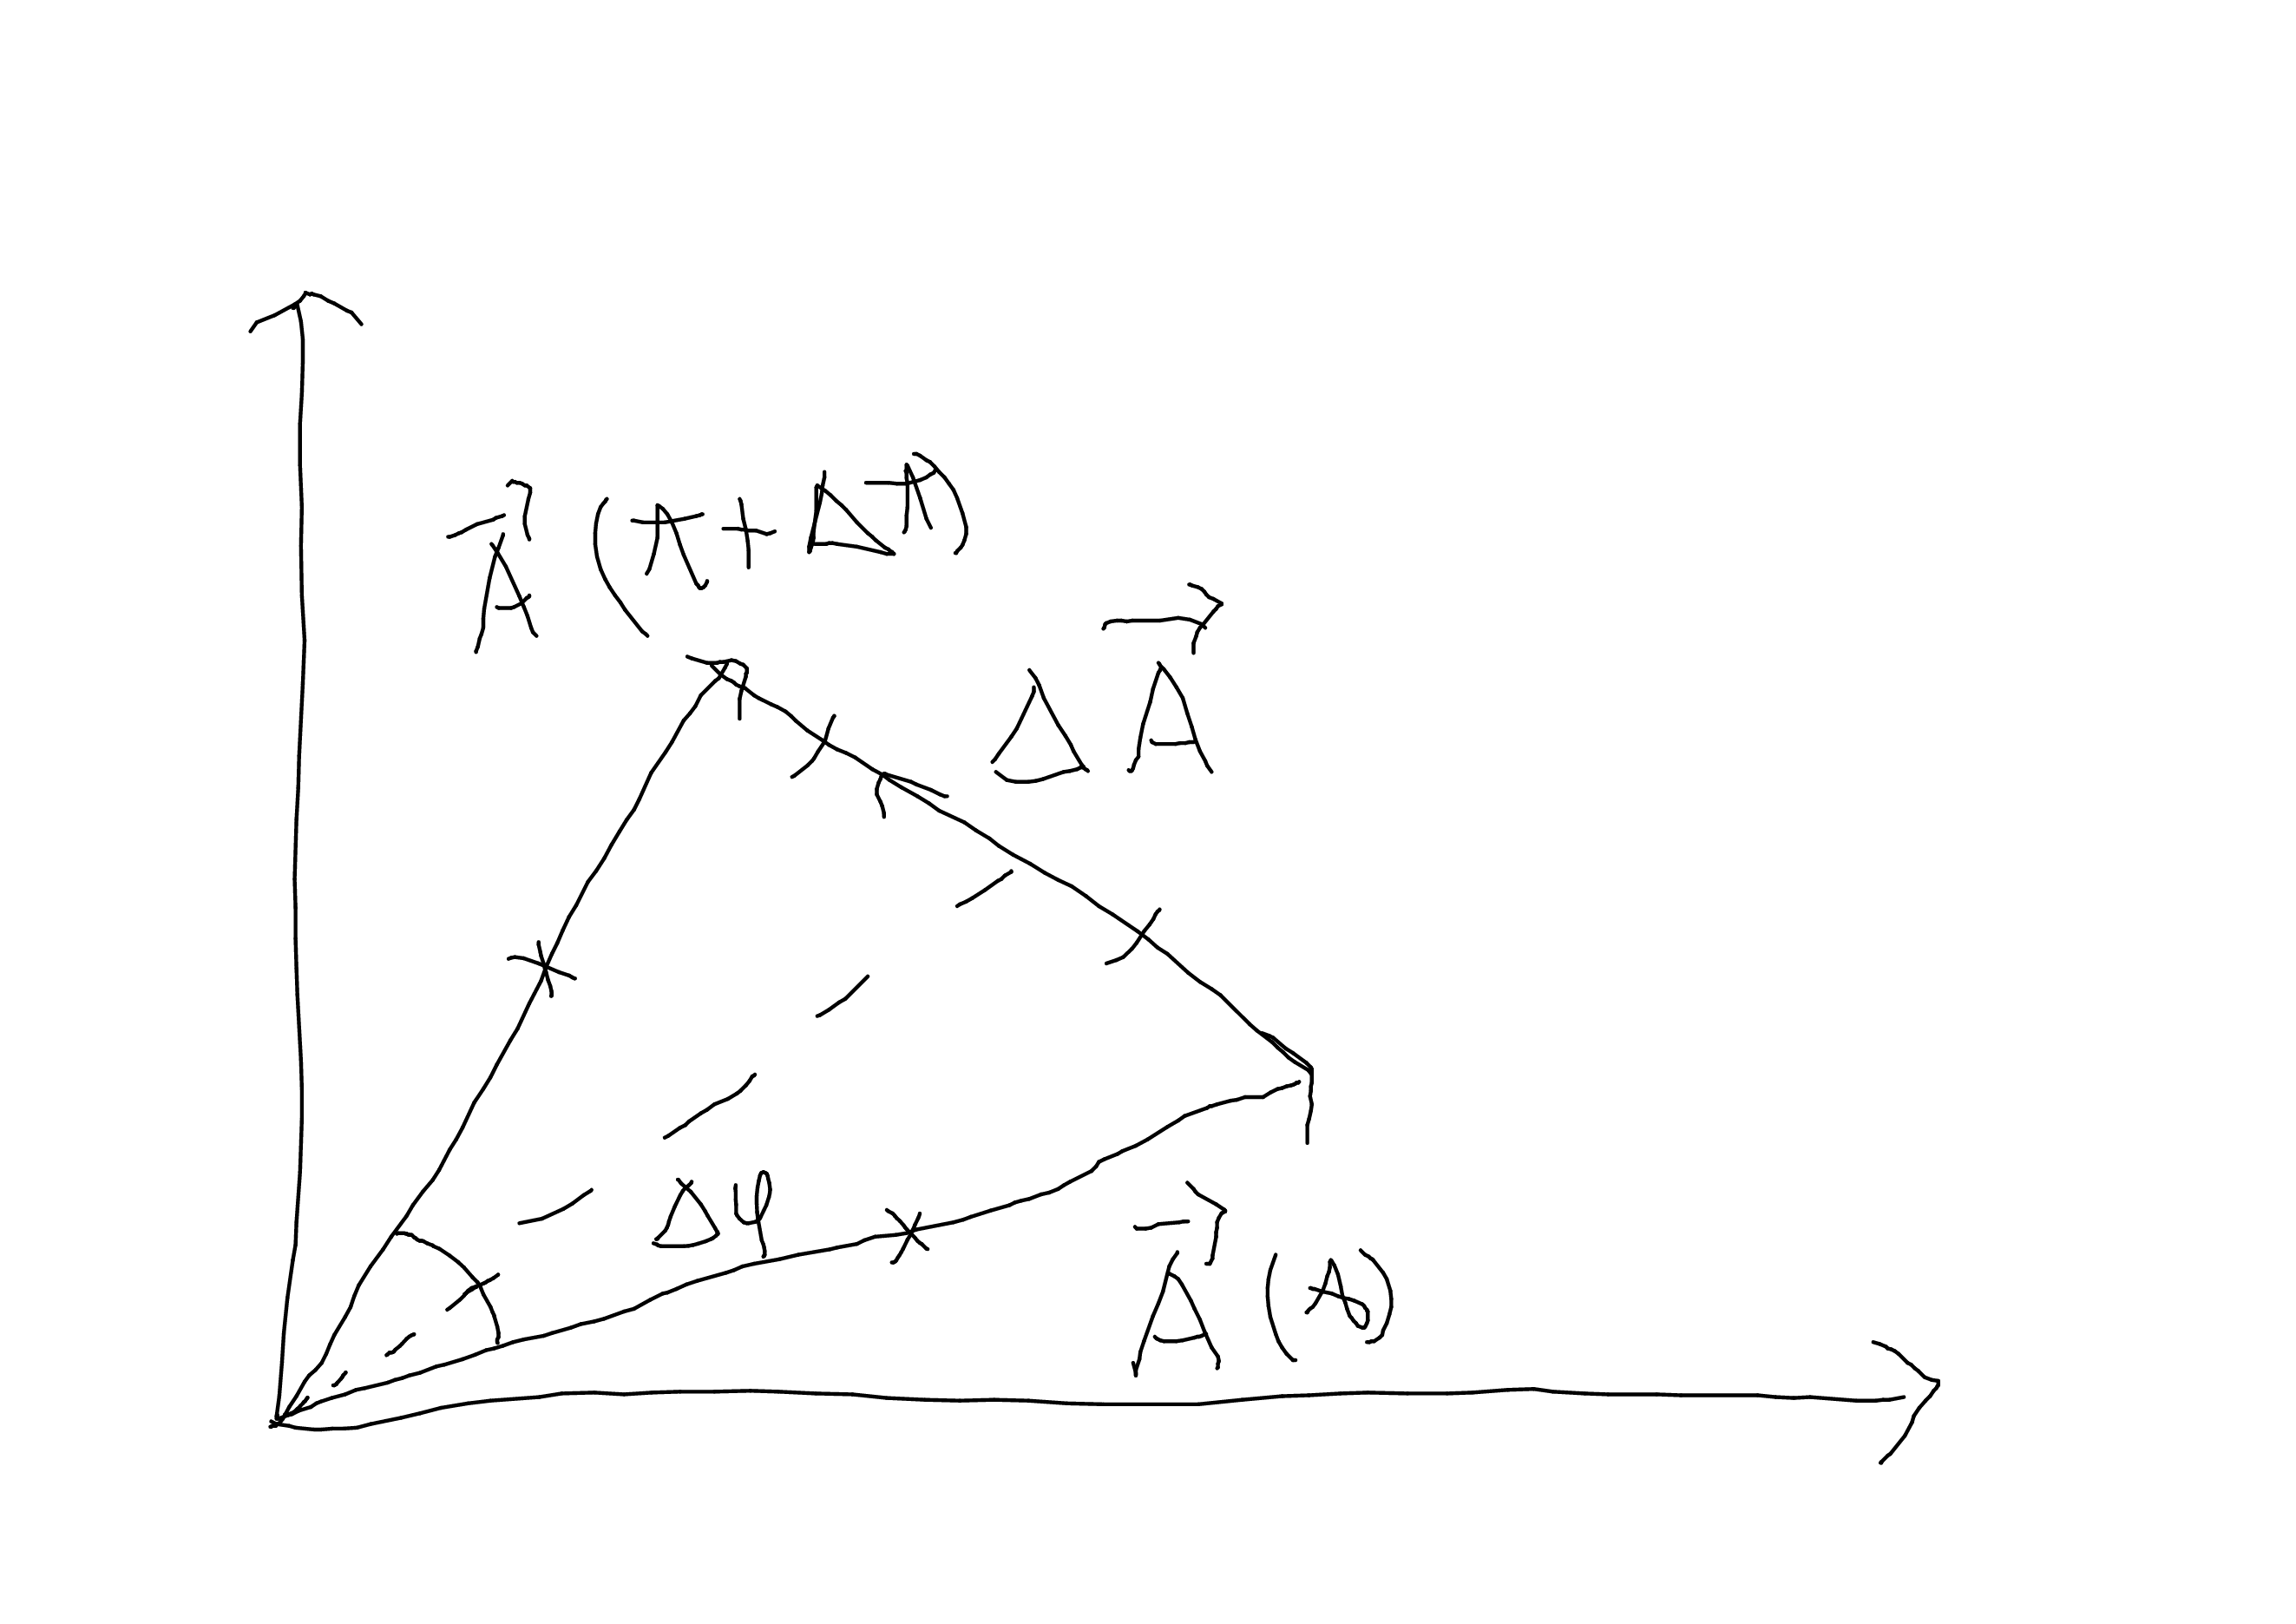
\includegraphics[width=0.5\textwidth]{VettRuotante.png}
\end{figure}
Pertanto possiamo esprimere il modulo del vettore variazione usando le proprietà dei triangoli come segue:
\[\abs{\Delta\va{A}}=2\abs{\A(t)}\sin\frac{\Delta\phi}{2}\]
Per calcolare la derivata calcoliamo il limite del rapporto incrementale, definiamo inoltre il versore $\normvs$ perpendicolare ad $\A$ in ogni istante e il versore $\normvs'$ invece parallelo:
\begin{equation}
\begin{split}
    \dv{\A}{t}&=\lim\limits_{\Delta t\to0}\frac{\Delta\A}{\Delta t}=\\
    &=\lim\limits_{\Delta t\to0}\frac{abs{\Delta\A}\normvs'}{\Delta t}=\\
    &=\lim\limits_{\Delta t\to0}\left[2\frac{\abs{\A(t)}}{\Delta t}\sin\frac{\Delta\phi}{2}\normvs'\right]=\\
    &=\abs{\A(t)}\lim\limits_{\Delta t\to0}\left[\frac{2}{\Delta t}\sin\frac{\Delta\phi}{2}\normvs'\right]=\\
    &=\abs{\A(t)}\lim\limits_{\Delta t\to0}\left[\frac{2}{\Delta t}\sin\frac{\Delta\phi}{2}\frac{\Delta\phi}{\Delta\phi}\normvs'\right]=\\
    &=\abs{\A(t)}\lim\limits_{\Delta t\to0}\left[\frac{\Delta\phi}{\Delta t}\frac{\sin\frac{\Delta\phi}{2}}{\frac{\Delta\phi}{2}}\normvs'\right]=\\
    &=\abs{\A(t)}\lim\limits_{\Delta t\to0}\left[\frac{\Delta\phi}{\Delta t}\normvs'\right]=\\
    &=\abs{\A(t)}\dv{\phi}{t}\normvs
\end{split}
\end{equation}
Ossia il versore $\normvs'$ per piccoli intervalli $\dif t$ approssima $\normvs$.
Possiamo poi definire la \textbf{velocità angolare} $\omega$ e l'accelerazione angolare $\alpha$:
\[\omega=\dv{\phi}{t}\quad\quad\alpha=\dv{\omega}{t}=\dv[2]{\phi}{t}\]
Otteniamo infine la seguente scrittura:
\begin{equation}
    \boxed{\dv{\A}{t}=\omega\abs{\A(t)}\normvs}
\end{equation}
\hypertarget{vettoreruotante}{Possiamo infine introdurre il \textbf{vettore rotazione} $\va{\omega}$, costruito in modo tale da rispettare la seguente relazione}:
\[\dv{\A}{t}=\omega\times\A\]
Ossia un vettore che ha per modulo la velocità angolare del vettore ruotante, direzione perpendicolare e verso uscente dal piano che contiene i vettori $\A$ e $\dv{\A}{t}$.
\subsection{Velocità e Accelerazione in Funzione della Posizione}
Considerando i casi in cui possiamo ridurre posizione, velocità e accelerazione a degli scalari (ad esempio nei moti rettilinei, circolari o utilizzando l'ascissa curvilinea), possiamo facilmente ottenere una relazione "senza tempo" facendo le seguenti osservazioni:
\[a=\dv{v}{t}=\dv{v}{x}\dv{x}{t}=v\dv{v}{x}\then a\dif x=v\dif x\]
Integrando tra un'istante e l'altro:
\begin{equation}\label{parametraccelerazione}
\int_{x_0}^xa\dif x=\int_{v_0}^v\dif v=\frac{v^2-v_0^2}{2}
\end{equation}
\section{Moti Vari}
Avendo studiato i casi generali e l'evoluzione del vettore posizione, velocità e accelerazione nel piano possiamo studiare diversi tipi di moti dei corpi puntiformi.
\subsection{Moti Rettilinei}
Un moto è rettilineo se il vettore posizione è sempre parallelo a se stesso. 
\paragraph{Moto Rettilineo Uniforme}
Scegliendo un sistema di riferimento opportuno (con uno dei due assi parallelo alla direzione del moto), la legge oraria del moto rettilineo uniforme si riduce (rispetto alla velocità) a:
\begin{equation}
\begin{cases}
v=v_0\\
x=x_0+v_0t
\end{cases}
\end{equation}
In generale vale comunque:
\begin{equation}
\begin{cases}
\v=\v_0\\
\r=\r_0+\v_0t
\end{cases}
\end{equation}
\paragraph{Moto Rettilineo Uniformemente Accelerato}
Per ottenere la legge oraria integriamo l'accelerazione rispetto al tempo:
\begin{equation}
\begin{cases}
\a=\a_0\\
\v=\v_0+\a_0t\\
\r=\r_0+\v_0t+\frac{\a_0}{2}t^2
\end{cases}
\end{equation}
Che si riduce con un'opportuna scelta di assi:
\begin{equation}
\begin{cases}
a=a_0\\
v=v_0+a_0t\\
x=x_0+v_0t+\frac{a_0}{2}t^2
\end{cases}
\end{equation}
\subsection{Moto Parabolico}
Il moto parabolico è il moto piano di un corpo composto da un moto rettilneo uniforme lungo una direzione e un moto rettilineo uniformemente accelerato nell'altra. Tipicamente è anche noto come \textbf{moto del proiettile}, in quanto un proiettile si muove (ignorando l'attrito) di un moto che si può scomporre orizzontalmente come moto rettilineo uniforme e verticalmente come moto uniformemente accelerato.\\
Scegliendo un'appropriato sistemo di riferimento otteniamo quindi (con velocità iniziale $\v_0$ inclinata di un angolo $\alpha$ rispetto all'orizzontale):
\begin{equation}
\begin{cases}
a_x=0\\
a_y=-g\\
\end{cases}\then
\begin{cases}
v_x=v_{0}\cos\alpha\\
v_y=v_0\sin\alpha-gt
\end{cases}\then
\begin{cases}
x(t)=x_0+v_0\cos\alpha\\
y(t)=y_0+v_0\sin\alpha-\frac{g}{2}t^2
\end{cases}
\end{equation}
Di particolare importanza sono i seguenti valori:
\begin{enumerate}
    \item Il Punto di Massima Altezza, raggiunto quando $v_y=0$
    \item Il Tempo di Volo $t_v$, ottenuto per $x(t_v)=0$
    \item La Gittata $L=x(t_v)-x_0$
\end{enumerate}
Inoltre possiamo applicare la \ref{parametraccelerazione} rispetto alla direzione verticale per ottenere una relazione "senza tempo":
\begin{equation}
    \int_{y_0}^ya(y)\dif y=-g(y-y_0)=\frac{v^2-v_0^2}{2}\then v(y)=\pm\sqrt{v_0^2-2g(y-y_0)}
\end{equation}
\subsection{Moto Armonico}
Un moto armonico è un moto descritto dalla seguente equazione differenziale:
\begin{equation}
    \boxed{\ddot{x}+\omega^2x=f(t)}
\end{equation}
Considerando il caso in cui $f(t)=0$ la soluzione generale (ponendo le condizioni iniziali $v(0)=v_0$ e $x(0)=x_0$):
\begin{equation}
    x(t)=x_0\cos{\omega t}+\frac{v_0}{\omega}\sin{\omega t}
\end{equation}
Questa può anche scriversi nella seguente forma ponendo opportune posizioni:
\begin{equation}
    x(t)=A\sin\left(\omega t+\phi_0\right)\quad\begin{cases}
    A=\sqrt{x_0^2+\left(\frac{v_0}{\omega}\right)^2}\\
    \tan\phi_0=\frac{x_0\omega}{v_0}
    \end{cases}
\end{equation}
Infatti ponendo le seguenti posizioni:
\[A\cos\phi_0=\frac{v_0}{\omega}\quad A\cos\phi_0=x_0\quad A^2=x_0^2+\frac{v_0^2}{\omega^2}\]
Otteniamo:
\begin{equation}
\begin{split}
    x(t)&=x_0\cos(\omega t)+\frac{v_0}{\omega}\sin(\omega t)=\\
    &=A\sin\phi_0\cos(\omega t)+A\cos\phi_0\sin(\omega t)=\\
    &=A\left[\sin\phi_0\cos(\omega t)+\cos\phi_0\sin(\omega t)\right]=\\
    &=A\sin(\omega t+\phi_0)
\end{split}
\end{equation}
Il \textbf{periodo} del moto armonico si ottiene dalla relazione:
\[\omega=\frac{2\pi}{T}\then\boxed{T=\frac{2\pi}{\omega}}\]

\subsection{Moti Circolari}
Un moto piano si dice circolare quando la sua traiettoria determina una circonferenza (o una sua parte, come nel caso del pendolo). Usando le proprietà del vettore ruotante, otteniamo:
\begin{equation}
\begin{cases}
    \r(t)=R\vu{r}\\
    \v(t)=\dv{\r(t)}{t}=R\dv{\vu{r}}{t}=\omega R\vu{t}=v_s(t)\vu{t}\\
    \a(t)=\dv{\v(t)}{t}=R\dv{\omega\vu{t}}{t}=R\Dot{\omega}\vu{t}-R\omega^2\vu{r}=a_s\vu{t}-\frac{v_s^2}{R}\vu{r}
\end{cases}
\end{equation}
Dove $\vu{t}$ è il vettore tangente (perpendicolare ad $\r$). In generale i versori, $a_s$, $v_s$ sono tutte funzioni di t.\\
I due moti circolari più rilevanti sono il \textbf{moto circolare uniforme} e il \textbf{moto circolare uniformemente accelerato}. L'ascissa curvilinea ci permette inoltre di studiare il moto tangenziale indipendentemente da quello centripeto. Utilizzando la proprietà della circonferenza $s(t)=R\phi(t)$ possiamo inoltre esprimere anche la rotazione (accelerazione, velocità e angolo spazzato).

\paragraph{Moto Circolare Uniforme}
Le leggi oraria del moto circolare uniforme rispetto all'ascissa curvilinea e vettorialmente sono le seguenti:
\begin{equation}
\begin{cases}
    s(t)=s_0+v_0t\\
    v_s(t)=v_0\\
    a_s(t)=0
\end{cases}\iff
\begin{cases}
    \r(t)=R\vu{r}
    \v(t)=R\omega\vu{t}=v_0\vu{t}\\
    \a(t)=-R\omega^2\vu{r}=-\frac{v_0^2}{R}\vu{r}
\end{cases}
\end{equation}
Infatti per il moto circolare uniforme $\abs{\a_{\tau}(t)}=0\then \abs{\a(t)}=\frac{v_0^2}{R}$.
\paragraph{Moto Circolare Uniformemente Accelerato}
Per il moto circolare uniformemente accelerato le leggi orarie sono le seguenti:
\begin{equation}
\begin{cases}
    s(t)=s_0+v_0t+\frac{1}{2}a_0t^2\\
    v_s(t)=v_0+a_0t\\
    a_s(t)=a_0
\end{cases}\iff
\begin{cases}
    \r(t)=R\vu{r}\\
    \v(t)=R\omega\vu{t}=(v_0+a_0t)\vu{t}\\
    \a(t)=R\Dot{\omega}\vu{t}-R\omega^2\vu{r}=a_0\vu{t}-\frac{(v_0+a_0t)^2}{R}\vu{r}
\end{cases}
\end{equation}
Potendo scomporre l'accelerazione in una componente radiale e una tangenziale ha particolare importanza conoscere il comportamento dell'angolo tra l'accelerazione e l'asse radiale (e quindi la componente centripeta). Schematizzando otteniamo la seguente figura:
\begin{figure}[H]
    \centering
    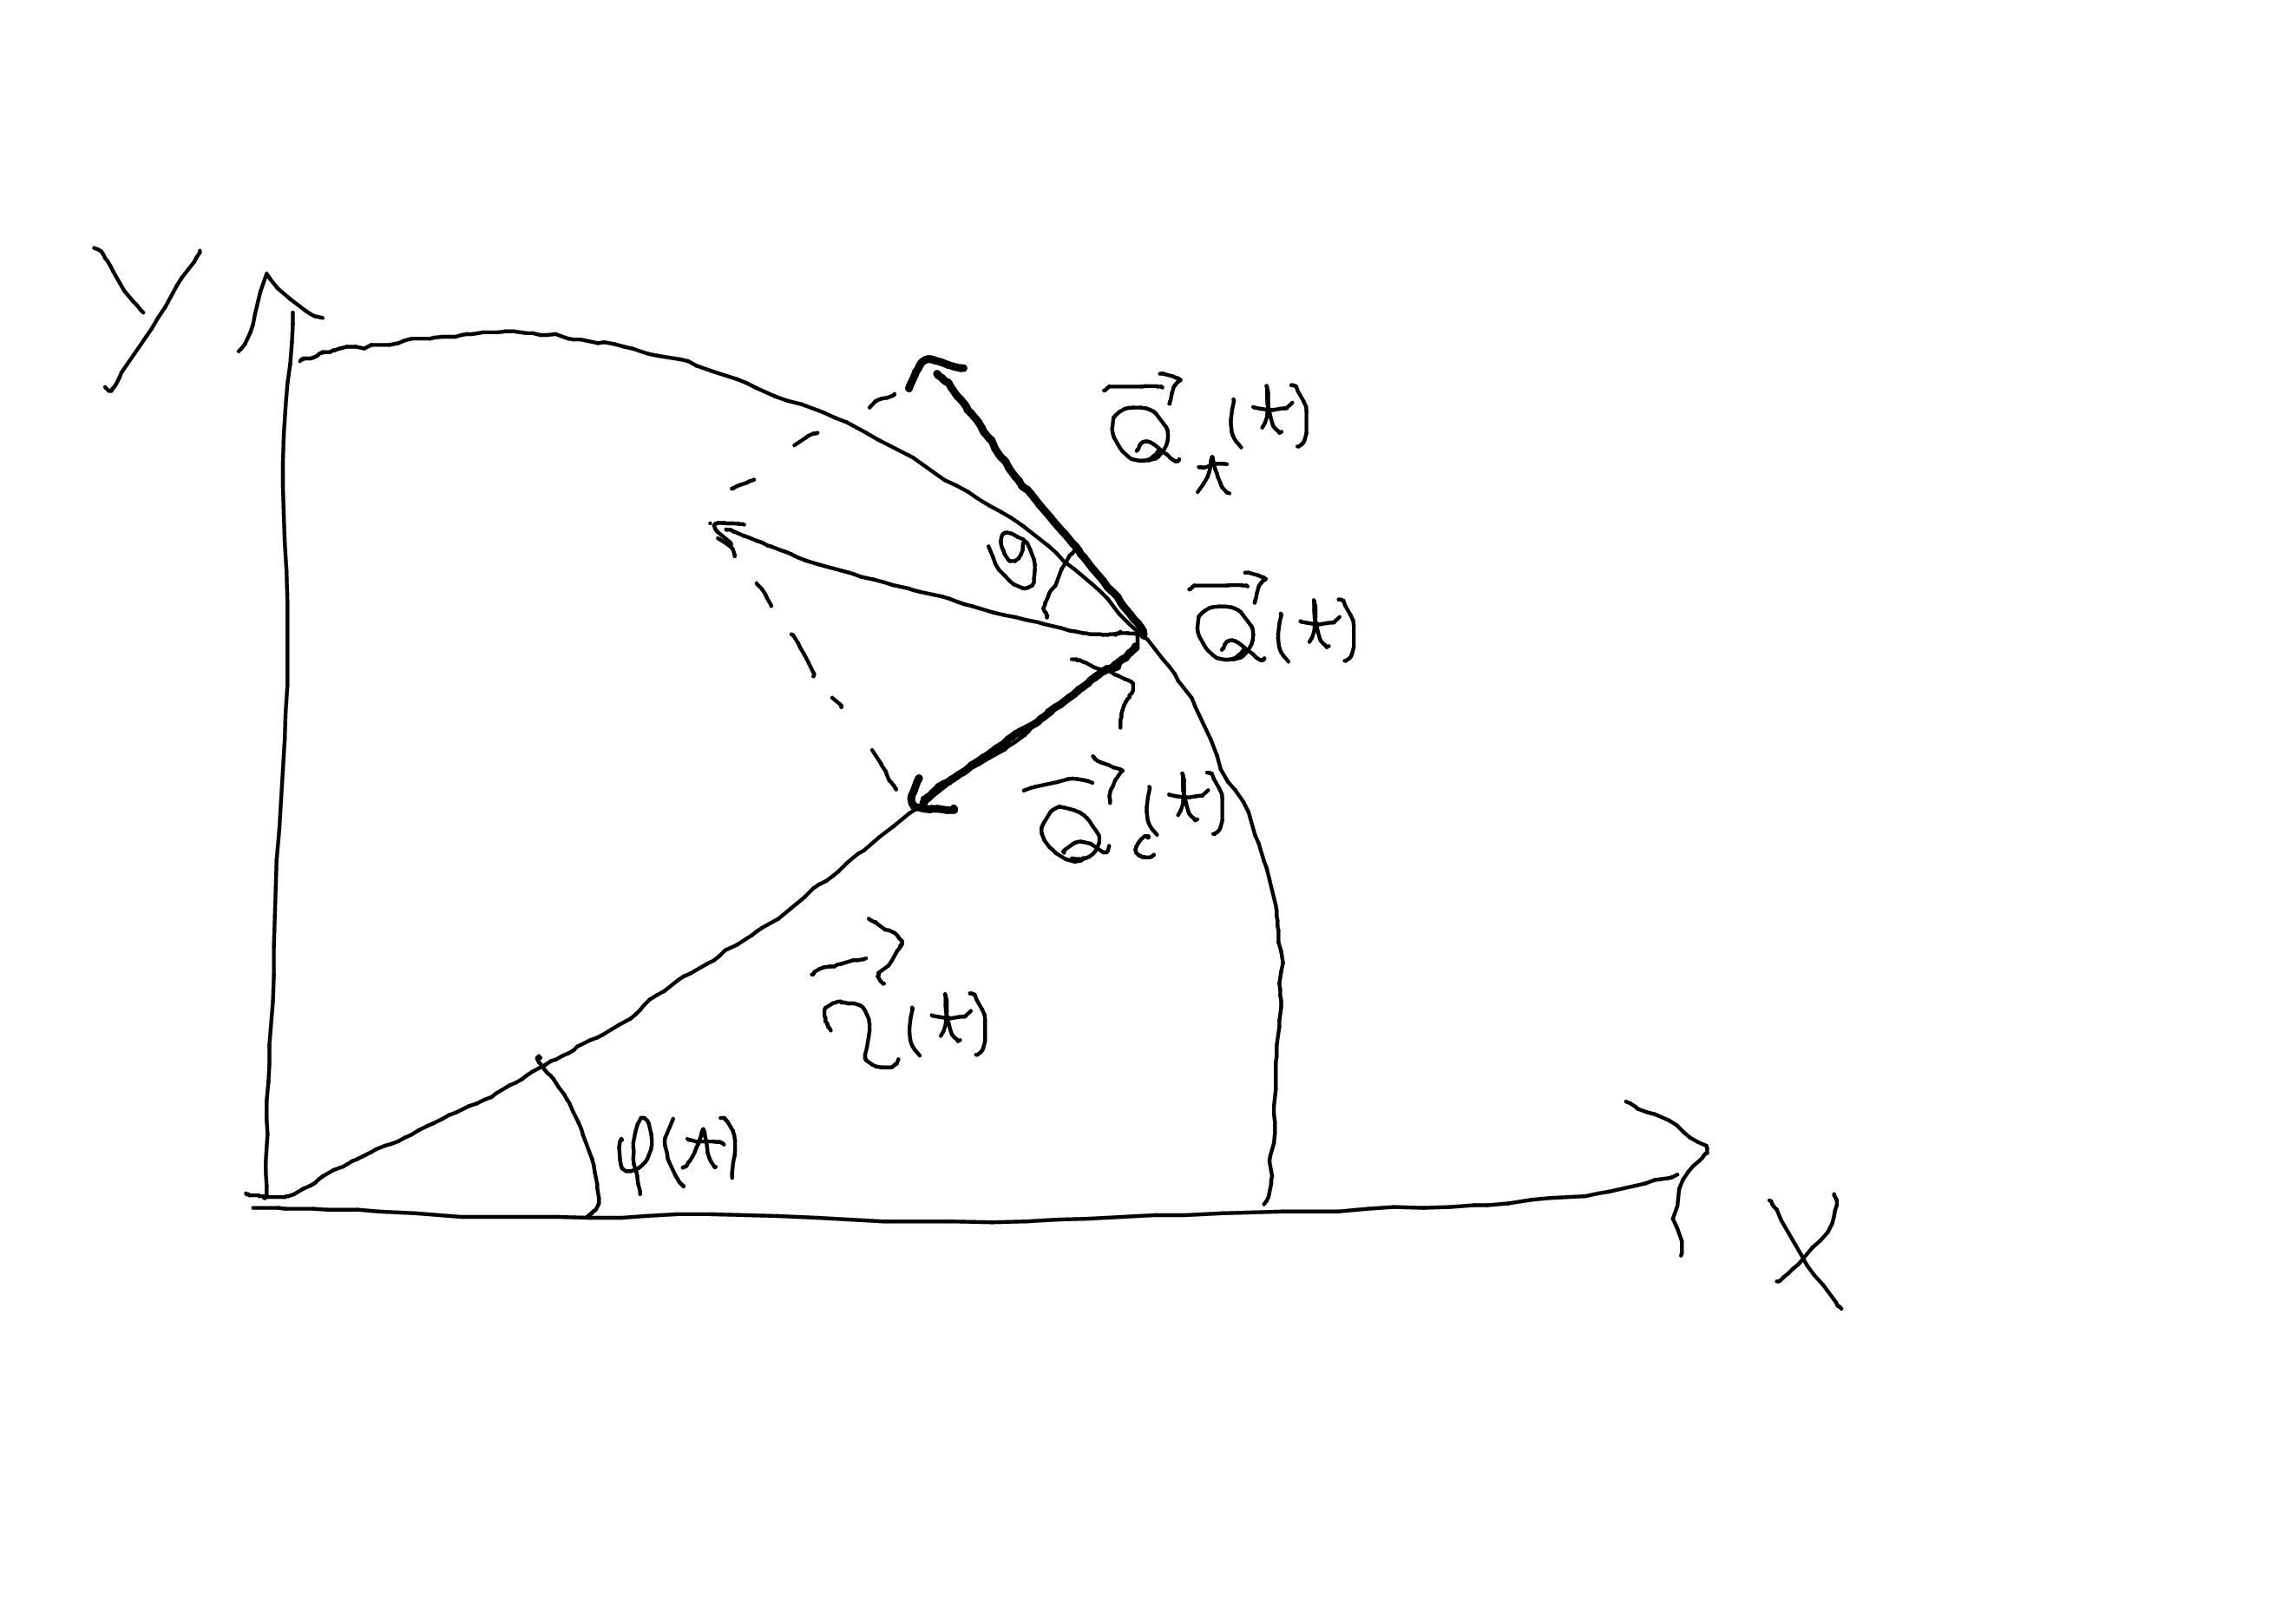
\includegraphics[width=0.5\textwidth]{AngoloAccCirc.png}
\end{figure}
Pertanto otteniamo:
\begin{equation}
\begin{cases}
    \abs{\a_c}=\abs{\a}\sin\theta\\
    \abs{\a_t}=\abs{\a}\cos\theta
\end{cases}\then \tan\theta=\frac{\abs{\a_c}}{\abs{\a_t}}
\end{equation}
Sviluppiamo:
\begin{equation}
\begin{split}
    \tan\theta&=\frac{\abs{\a_c}}{\abs{\a_t}}=\\
    &=\frac{(v_0+a_0t)^2}{Ra_0}=\\
\end{split}
\end{equation}
Nel caso in cui $s_0=0$ e $v_0=0$ otteniamo un utile relazione con l'ascissa curvilinea:
\[\tan\theta=\frac{a_0^2t^2}{Ra_0}=\frac{a_0t^2}{R}\then a_0t^2=R\tan\theta\then s(t)=\frac{1}{2}R\tan\theta\]
\chapter{Dinamica del Corpo Puntiforme}
\section{I Tre Principi}
I tre principi della dinamica sono i fondamenti per comprendere il moto dei corpi, partendo da quelli puntiformi fino alla costruzione del modello dei sistemi. 
Il primo principio o \textbf{principio d'inerzia}, già accennato nella cinematica, si enuncia come segue:
\begin{enunc}
Un corpo resta in stato di quiete o di moto rettilineo uniforme se la risultante delle forze agenti su di esso è nulla.
\end{enunc}
Per \textbf{forza} intendiamo quella grandezza capace di esprimere e quantificare l'Interazione tra corpi, la conseguenza di tali interazioni viene spiegata dal secondo e terzo principio della dinamica. Una forza per agire non deve quindi necessariamente provocare uno spostamento, possiamo quindi definire la forza \textbf{staticamente} (calcolarne l'intensità, direzione e verso).
\paragraph{Definizione Operativa della Forza Statica}
Per misurare la forza statica possiamo servirci del \textbf{dinamometro a deformazione}, ossia una molla tarata. Per tarare questa molla utilizziamo una riga, poniamo lo zero in corrispondenza dell'estremo libero quando non agisce alcuna forza sulla molla; poi scegliamo una forza campione, ad esempio collegando una certa massa all'estremo libero, in modo da esercitare la forza-peso di quel corpo sull'estremo libero, segniamo quindi "1" in corrispondenza dell'allungamento ottenuto. Collegando un altro corpo avente lo stesso peso unitario (ossia che produce lo stesso allungamento) otterremo un allungamento che corrisponde a circa il doppio di quello iniziale, a cui assoceremo "2". Abbiamo quindi prodotto una scala con cui possiamo misurare le intensità delle forze. 
\begin{enunc}[Secondo Principio della Dinamica]
L'interazione di un corpo puntiforme misurata dalla forza $\F$ con altri corpi determina l'accelerazione del punto secondo una costante \textit{m}, detta \textbf{massa inerziale}.
\[\F=m\a\]
\end{enunc}
Il secondo principio chiarisce quindi il caso in cui la risultante delle forze \textbf{non} sia nulla, producendo un'accelerazione che è inversamente proporzionale alla massa di quel corpo. La massa inerziale rappresenta quindi una misura di un corpo ad \textit{opporsi} all'accelerazione. Vediamo ora come definire operativamente questa grandezza.
\paragraph{Definizione Operativa della Massa Inerziale}
Per misurare questa grandezza utilizziamo il \textbf{carrello delle masse}, costituito da un carrello collegato ad una molla posizionati entrambi in orizzontale su un piano tarato, su cui possiamo misurare gli spostamenti. Per misurare la massa di un oggetto lo poniamo sul carrello, comprimendolo o allungandolo di una certa lunghezza, misuriamo quindi il periodo del moto armonico risultante. Osserviamo che il periodo del moto dipende unicamente dalla massa, quindi due corpi messi in moto sul carrello delle massa hanno lo stesso periodo posseggono anche la stessa massa. 
%Tuttavia questo metodo di misurazione non fornisce dati quantitativi e una scala con cui misurare altre massa, ma solo dati qualitativi.
\\
Alternativamente per misurare la massa di un oggetto possiamo utilizzare il terzo principio della dinamica. Esso si enuncia come segue:
\begin{enunc}[Terzo Principio della Dinamica]
Se un corpo A esercita una forza su un corpo B, il corpo B esercita sul corpo A una forza che agisce sulla stessa retta di azione (ossia la congiungente), ha stesso modulo e verso opposto.
\[\F_{A\to B}=-\F_{B\to A}\]
\end{enunc}
Utilizzando questo principio possiamo ricavare che due corpi che interagiscono accelerano secondo la seguente relazione:
\[\abs{\F_{A\to B}}=\abs{\F_{B\to A}}\iff m_A\abs{\a_A}=m_B\abs{\a_B}\then m_B=m_A\frac{\abs{\a_A}}{\abs{\a_B}}\]
Fissando la massa $m_A$ come campione possiamo misurare le due accelerazioni risultanti dall'interazioni e quindi stabilire il valore della massa di un corpo. Il campione utilizzato nel S.I. è una certa massa di \textit{platino-iridio}.\\
Dal terzo principio possiamo anche ricavare che per n corpi (un sistema isolato) valgono le seguenti relazioni:
\[\begin{cases}
    \sum_i^nm_i\a_i=0\\
    \sum_i(\r_i\times m_i\a_i)=0
\end{cases}\]


\section{Leggi di Forza}
Sebbene sia fondamentale enunciare i tre principi della dinamica, non sono sufficienti per studiare il moto dei corpi. Per fare ciò sono necessarie \textbf{Leggi di Forza}, ossia stabilire il valore e proprietà delle interazioni tra corpi.
\subsection{La Forza Gravitazionale}
Si osserva sperimentalmente che due corpi esercitano tra di loro un'interazione, detta \textbf{forza gravitazionale}, il cui modulo è inversamente proporzionale al quadrato della distanza tra i due e direttamente proporzionale al prodotto di due oggetti, dette \textbf{masse gravitazionali}. Più precisamente possiamo esprimere la forza gravitazionale con la seguente espressione matematica:
\[\F_{1\to2}=G\frac{m_1m_2}{|\r_{12}|^3}\r_{12}=G\frac{m_1m_2}{|\r_{12}|^2}\vu{r}_{12}\]
Quando si considera il moto di un corpo attorno alla terra, anch'essa esercita una certa forza gravitazionale, ma possiamo compiere una serie di approssimazioni in modo da semplificare la trattazione della forza-peso in situazioni che non richiedono alta precisione:
\begin{enumerate}
    \item Consideriamo il raggio della Terra come una costante
    \item Consideriamo piatta la parte della Terra coinvolta nell'esercizio
    \item Consideriamo la Terra un sistema inerziale, che non ruota attorno a se stessa e al Sole (in modo da dover considerare forze apparenti) 
    \item Consideriamo che la Terra non acceleri verso il corpo a causa della propria attrazione gravitazionale (approssimazione permessa dall'enorme differenza di massa gravitazionale tra il corpo e la Terra)
\end{enumerate}
La forza gravitazionale terrestre può essere quindi approssimata alla forma di \textbf{forza-peso}, espressa dalla seguente legge:
\[\F_p=m\va{g}\quad\abs{\va{g}}=9.8m/s^2\]
Chiamiamo il vettore $\va{g}$ l'accelerazione gravitazionale, verticale e diretto verso il basso (centro della Terra).
\subsection{Forze Vincolari}
Le forze vincolari sono forze dovute alla presenza di un vincolo, come può essere la lunghezza di un filo (tensione) o la non-compenetrazione di due corpi a contatto (forza normale). 
\paragraph{Tensione}
La tensione di un filo è una forza che si trova ogni qual volta si impone il vincolo che un filo rimanga in tensione, e quindi che la sua lunghezza sia costante. Tipici esempi includono il Pendolo Semplice e sistemi contenenti carrucole.\\
I vincoli possono esprimersi come seguono:
\[\f(\r,\v)=0\]
Un vincolo si dice \textbf{olonomo}, se il vincolo non è funzione della velocità; si dice invece \textbf{anolonomo} se lo è. Tramite il numero di vincoli possiamo anche calcolare il numero di \textbf{gradi di libertà}:
\[g.d.l=dimV_3-n_{vincoli}\]
\subparagraph{Pendolo Semplice}
Il pendolo semplice è il moto risultante da un corpo puntiforme appeso con un filo in oscillazione attorno al punto fisso cui è collegato il filo. Il secondo principio afferma che vale la seguente relazione:
\[m\g+\va{\tau}=m\a\]
Con $\va{\tau}$ tensione del filo.
\begin{figure}[H]
    \centering
    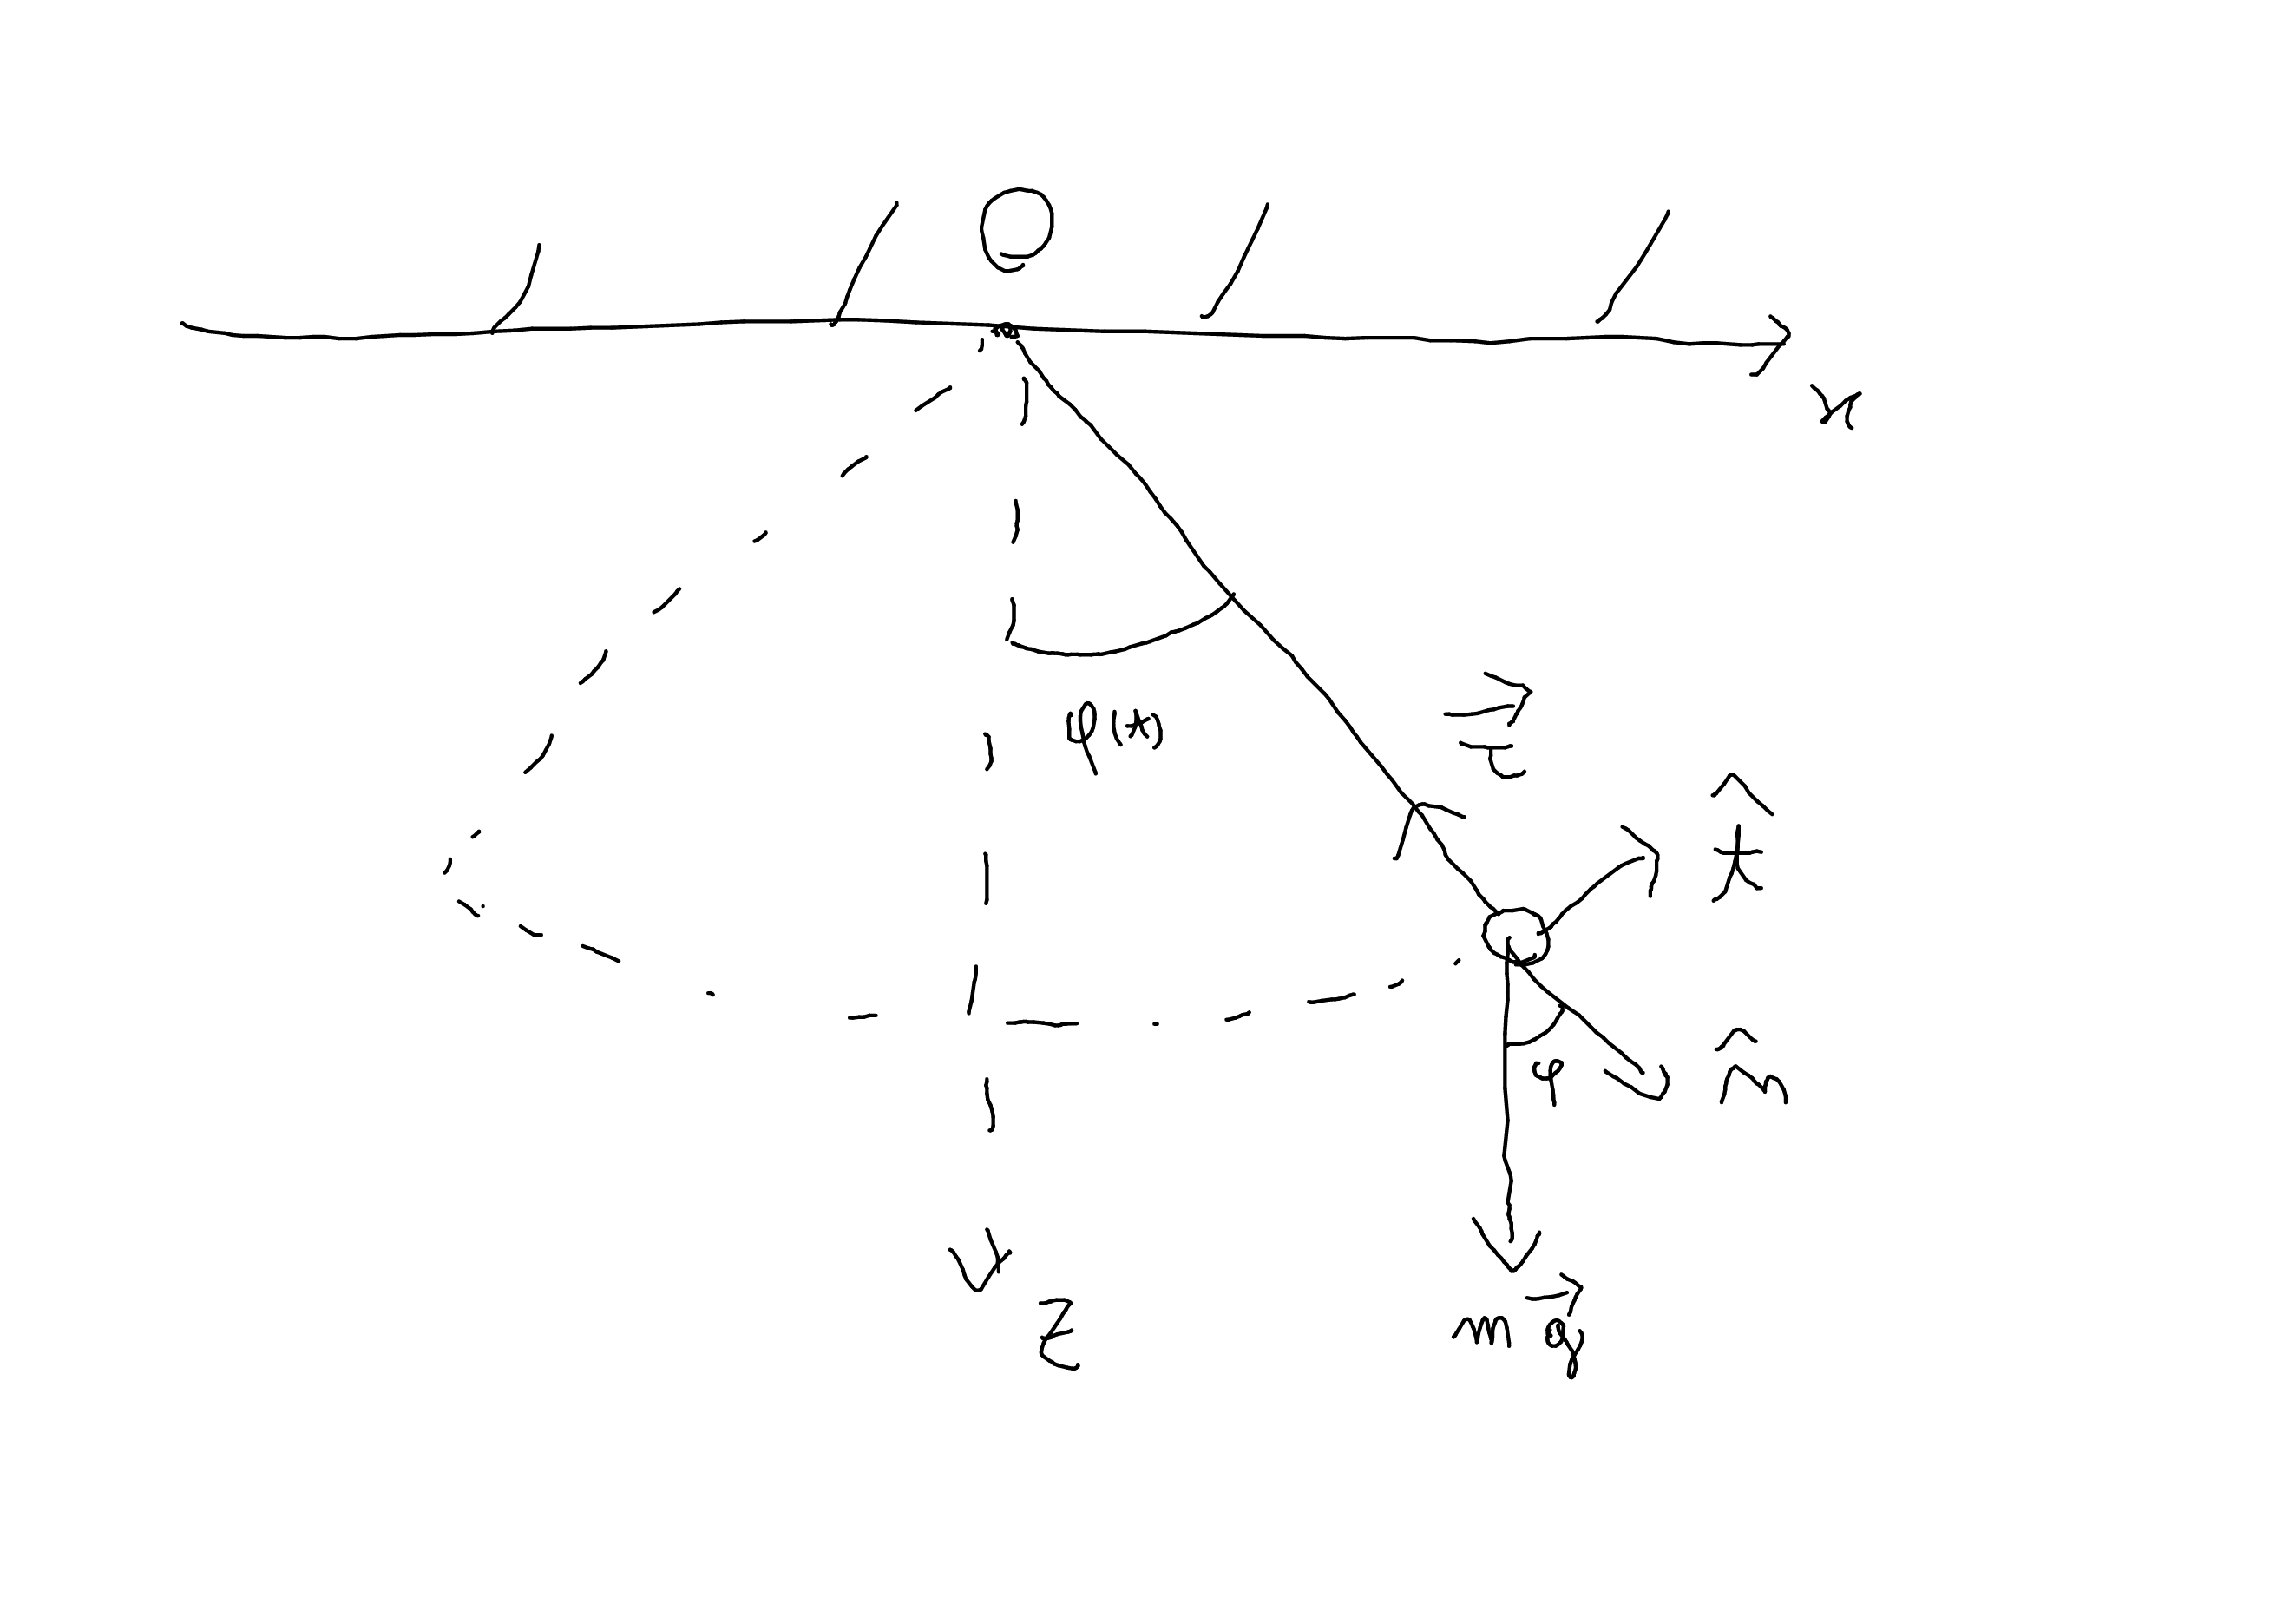
\includegraphics[width=0.5\textwidth]{PendoloSemplice.png}
    \caption{Esempio di Pendolo Semplice}
\end{figure}
Usando un sistema di riferimento solidale al corpo con componenti tangenziale e radiale/normale otteniamo:
\begin{align}
\vu{t})-mg\sin\phi=ma_s(t)=ml\ddot{\phi}\\
\normvs)mg\cos\phi-\abs{\tau}=-m\frac{v_s^2(t)}{l}=-ml\Dot{\phi}^2
\end{align}
Risolvendo otteniamo due equazioni differenziali:
\begin{equation}
\begin{cases}
    \ddot{\phi}+\frac{g}{l}\sin\phi=0\\
    \abs{\va{\tau}}=mg\cos\phi+ml\Dot{\phi}^2
\end{cases}
\end{equation}
Ammettendo l'ipotesi di piccole oscillazioni otteniamo $\sin\phi\approx\phi$ e quindi l'equazione si riconduce al moto armonico, che si può risolvere esattamente. Per piccole oscillazioni otteniamo quindi che il pendolo è \textbf{isocrono}, ossia il periodo del moto armonico (approssimato) è lo stesso indipendentemente dall'ampiezza. \\
Altre considerazioni rilevanti sul pendolo sono la condizione di allentamento del filo/distacco, dopo la quale il corpo si continua a muove di moto parabolico:
\[\boxed{\N=0}\iff mg\cos\phi=-ml\Dot{\phi}^2\then \boxed{\cos\phi=-\frac{\Dot{\phi}^2l}{g}}\]

\subsection{Forze d'Attrito}
Le leggi di forze delle forze d'attrito sono leggi sperimentali, in particolare quelle di contatto tra solidi si dividono tra due tipi: \textbf{statico} e \textbf{dinamico}. \\
Il secondo tipo è facile da descrivere in quanto tutte le informazioni sono note indipendentemente dal sistema e dalle forze agenti:
\begin{enumerate}
    \item Direzione Tangente alla Superficie di Contatto
    \item Verso Opposto al Moto Relativo alla Superficie
    \item Modulo di:
    \[\abs{\f_d}=\mu_d\abs{\N}\]
\end{enumerate}
L'attrito statico invece è un attrito di "equilibrio", in quanto il suo modulo e verso dipendono dalla risultante delle forze agenti sul corpo. Si osserva che la forza d'attrito ha un modulo massimo, entro il quale il corpo rimane in una situazione statica, superato questo valore il corpo entra in moto e quindi agisce l'attrito statico:
\[\abs{\f_s}\leq\mu_s\abs{\N}\]
Pertanto la forza d'attrito si comporta come segue in funzione del modulo delle forze risultanti agenti lungo la superficie di contatto:
\begin{figure}[H]
    \centering
    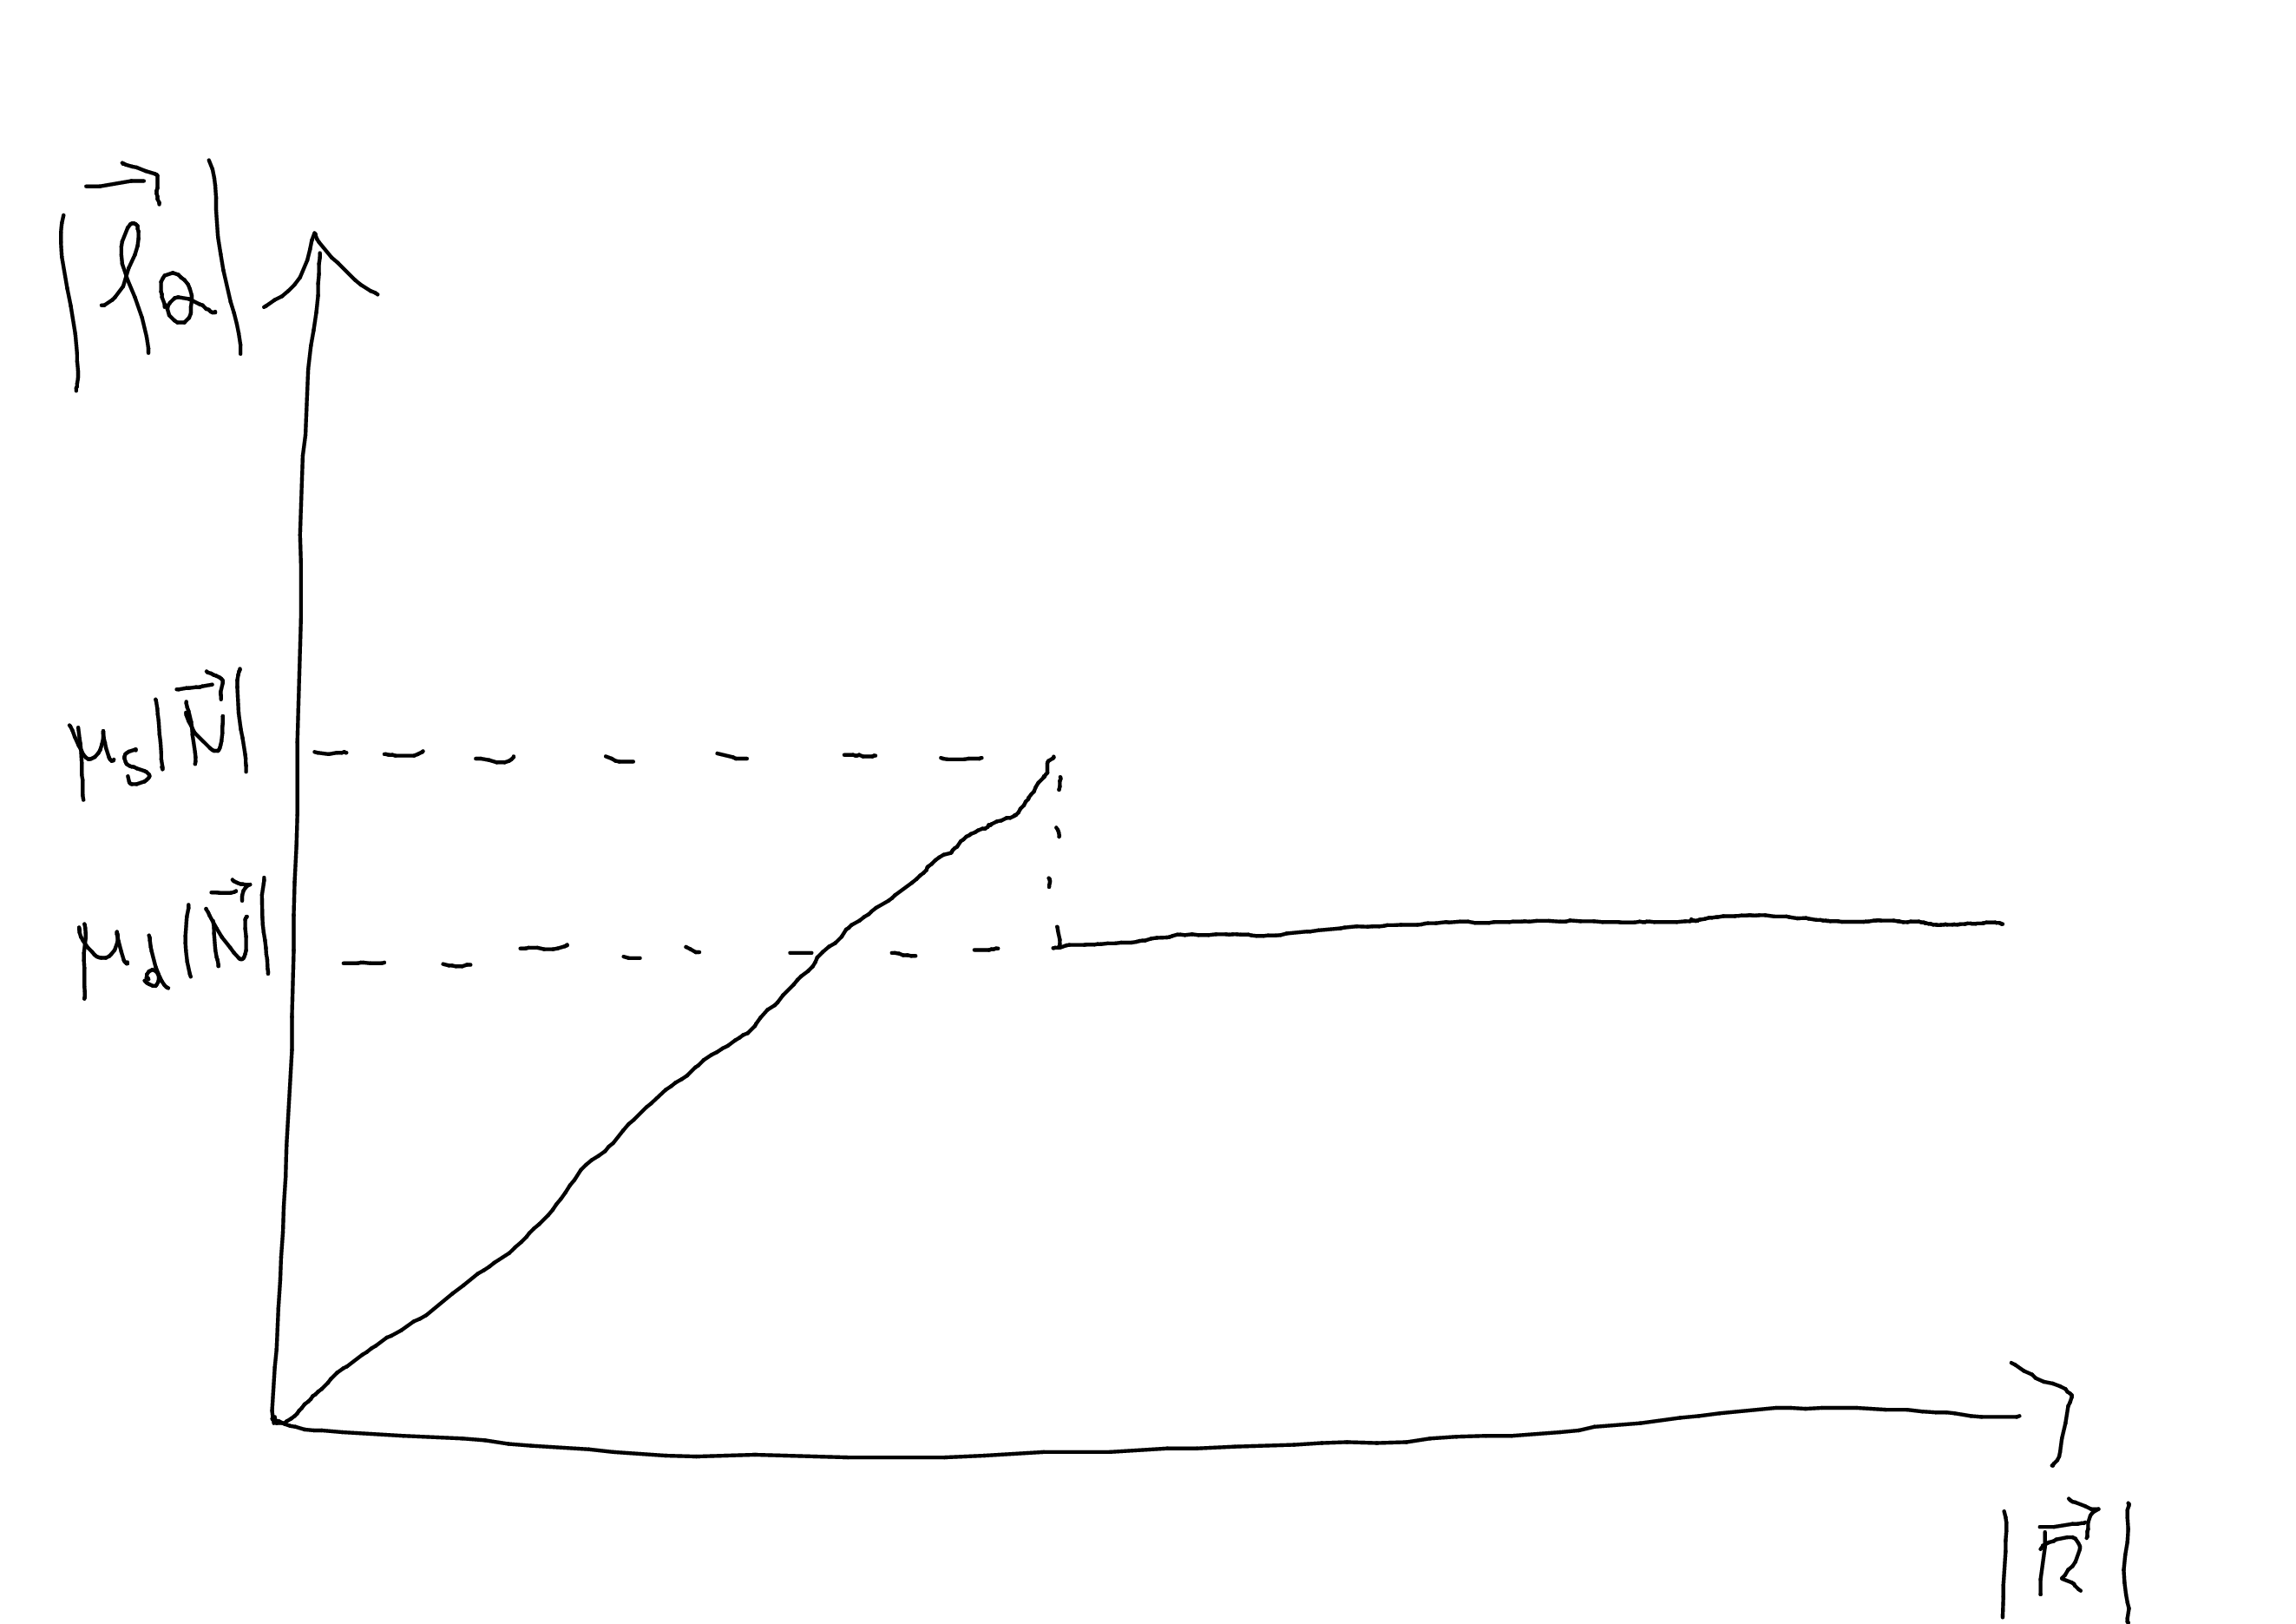
\includegraphics[width=0.5\textwidth]{Attrito.png}
\end{figure}


\subsection{Forza Elastica}
La forza elastica è la forza esercitata da una molla quando essa viene deformata (allungata o compressa) secondo la \textbf{Legge di Hooke}, valida per deformazioni non \textit{eccessive} e molle ideali:
\begin{enumerate}
    \item La direzione è parallela alla molla
    \item Il verso è opposto alla deformazione
    \item Il modulo è:
    \[\abs{\F_e}=k\abs{\Delta l}\]
\end{enumerate}
Un corpo soggetto ad una forza elastica si muove di moto armonico (semplice, forzato o smorzato a seconda dei casi). Un tipico esempio è quello di un corpo inizialmente in una situazione di deformazione collegato ad una molla e poggiato su un piano:
\begin{figure}[H]
    \centering
    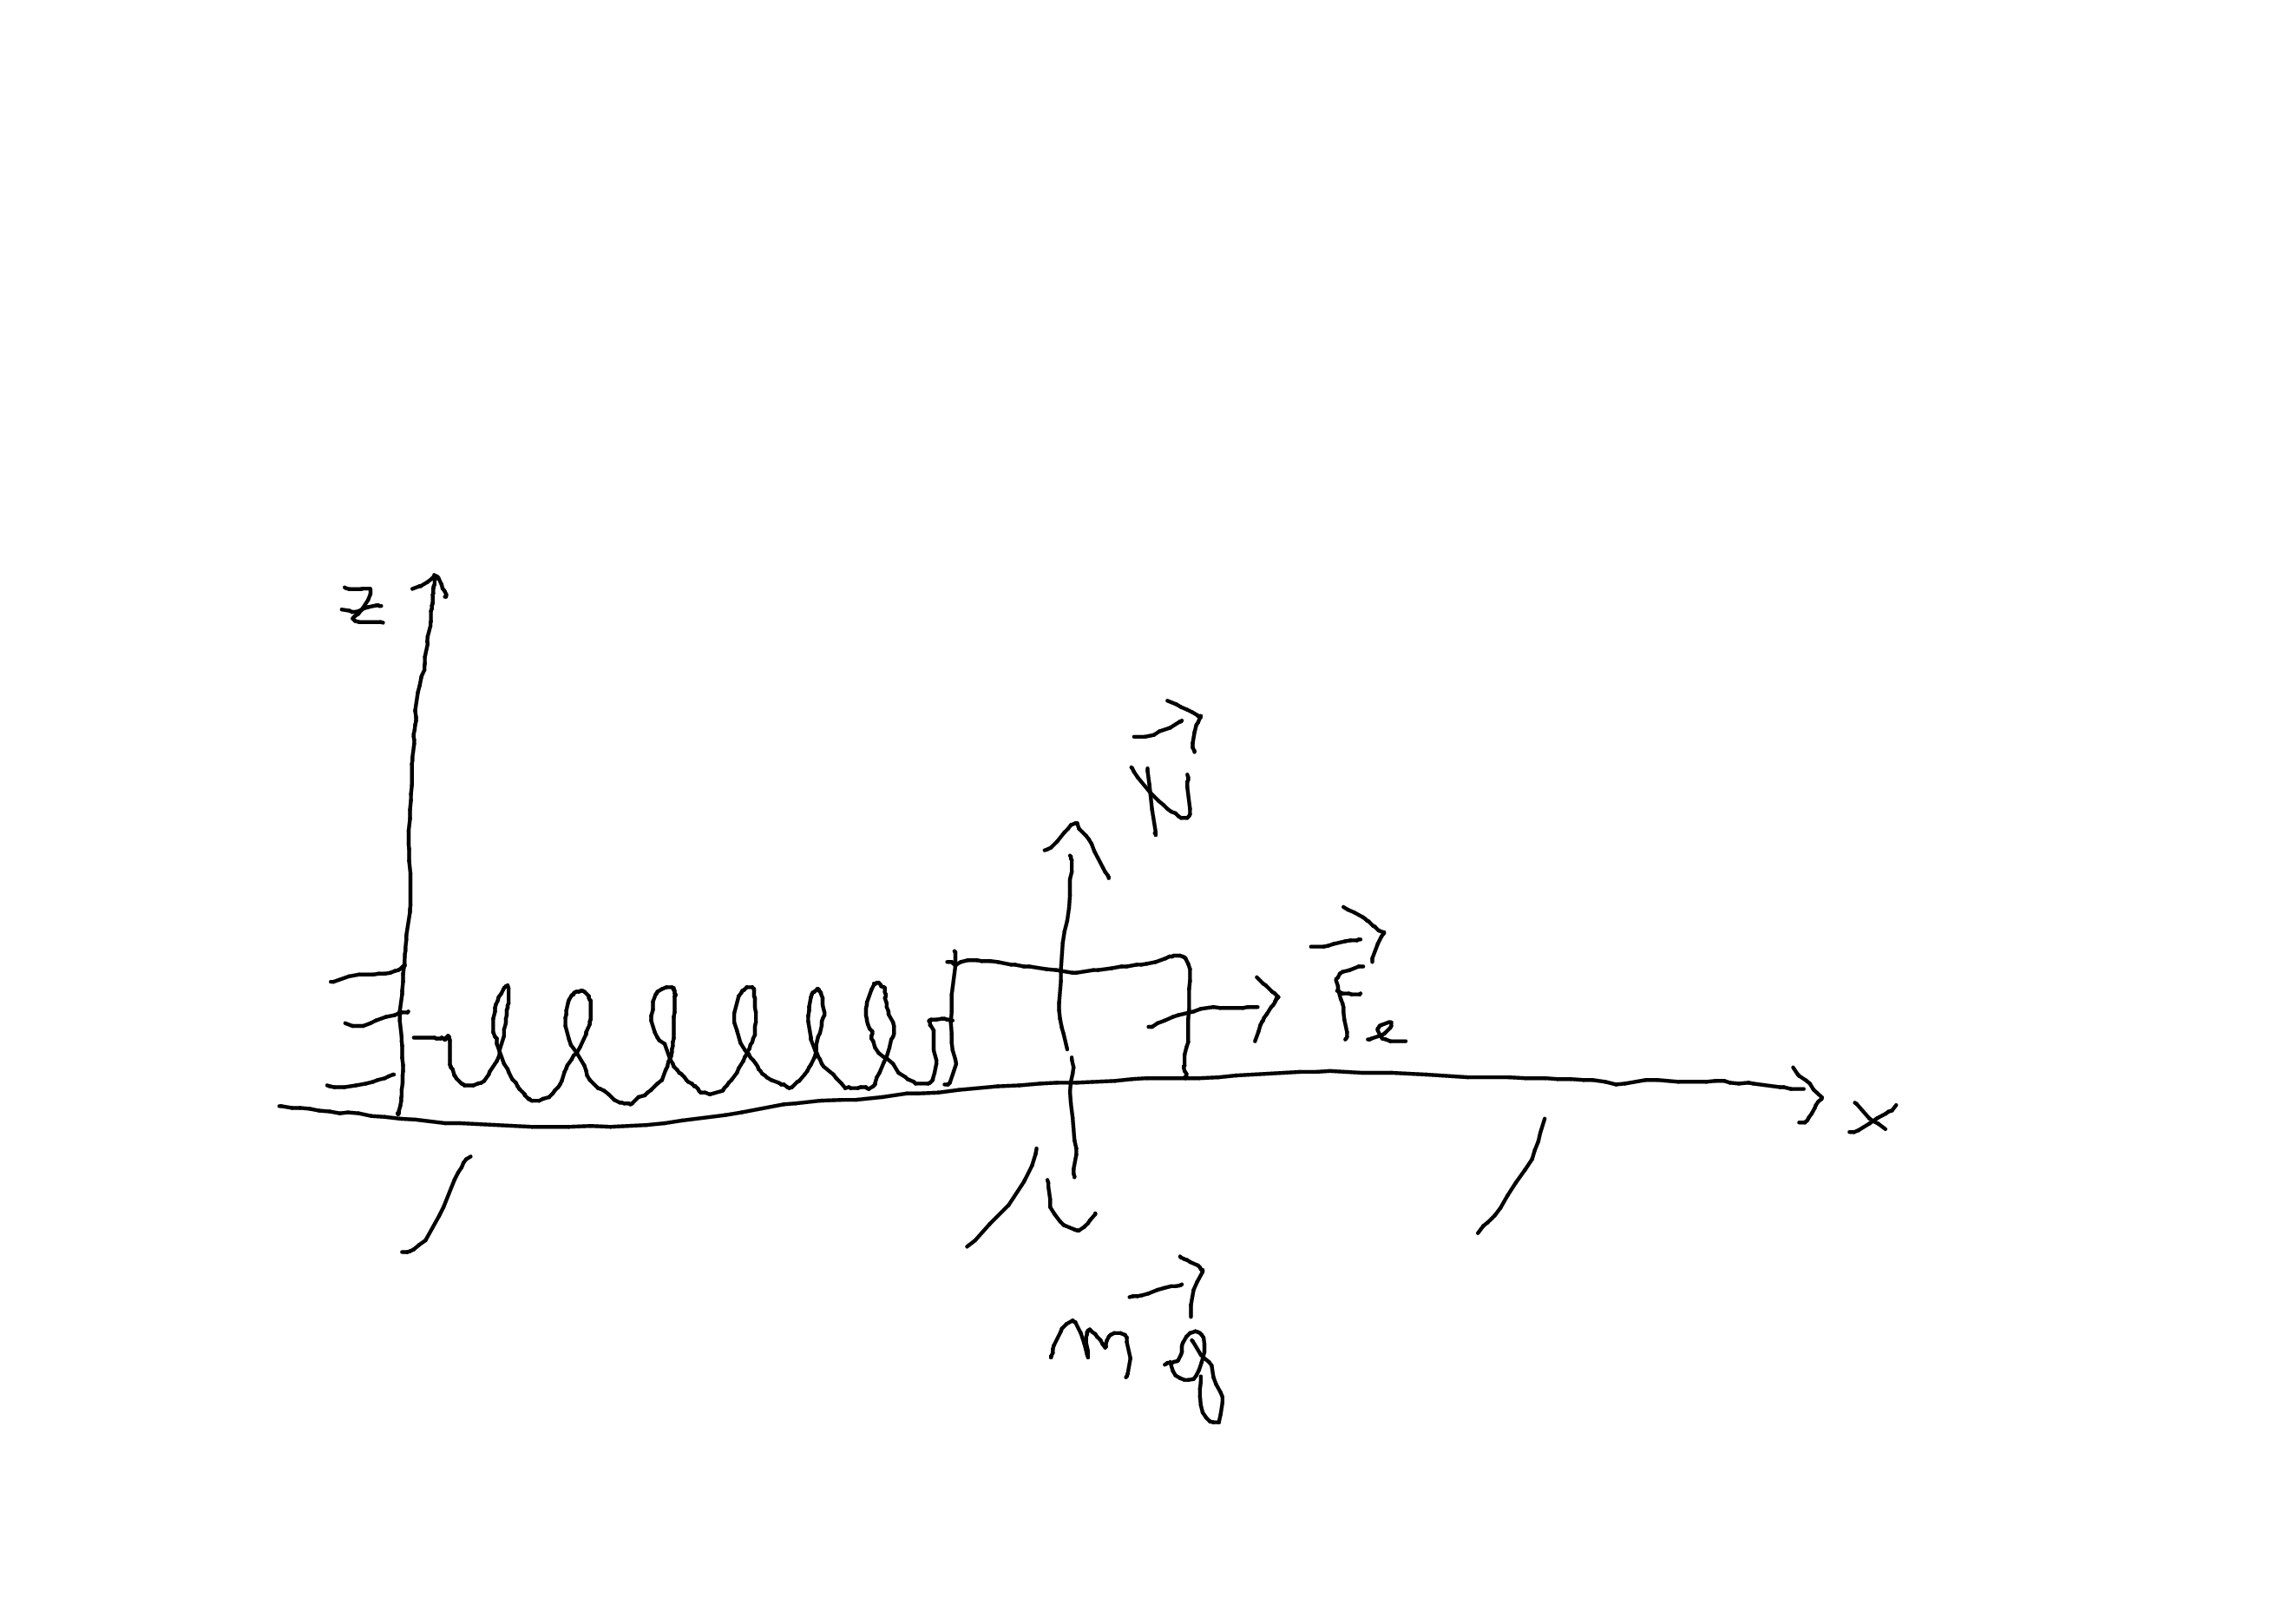
\includegraphics[width=0.5\textwidth]{ForzaElastica.png}
\end{figure}
Lo studio del moto si riduce quindi tutto sull'asse orizzontale:
\[-k(x-x_0)=m\ddot{x}\]
Da cui otteniamo l'equazione del moto armonico (esatto):
\[\ddot{x}+\omega^2x=0\quad\quad\omega=\sqrt{\frac{k}{m}}\]



\section{Le Trasformazioni Galileiane}
Un altro passo importante per la cinematica del corpo puntiforme è la possibilità di considerare posizioni, velocità e accelerazioni di un sistema diverso dal nostro note queste informazioni nel nostro sistema e il moto del sistema di riferimento.\\
A tale scopo sono necessarie \textbf{formule di composizione} per posizione, velocità e accelerazione. 
\subsection{Formule di Composizione}
Consideriamo il caso generale di un sistema K' di moto \textbf{roto-traslatorio}, ossia tale che la posizione del centro O' cambia rispetto al sistema \textbf{fisso} K e i vettori $\i',\j',\k'$ non restano paralleli a se stessi nel tempo. Consideriamo prima di tutto la posizione, abbastanza intuitivamente otteniamo:
\begin{figure}[H]
    \centering
    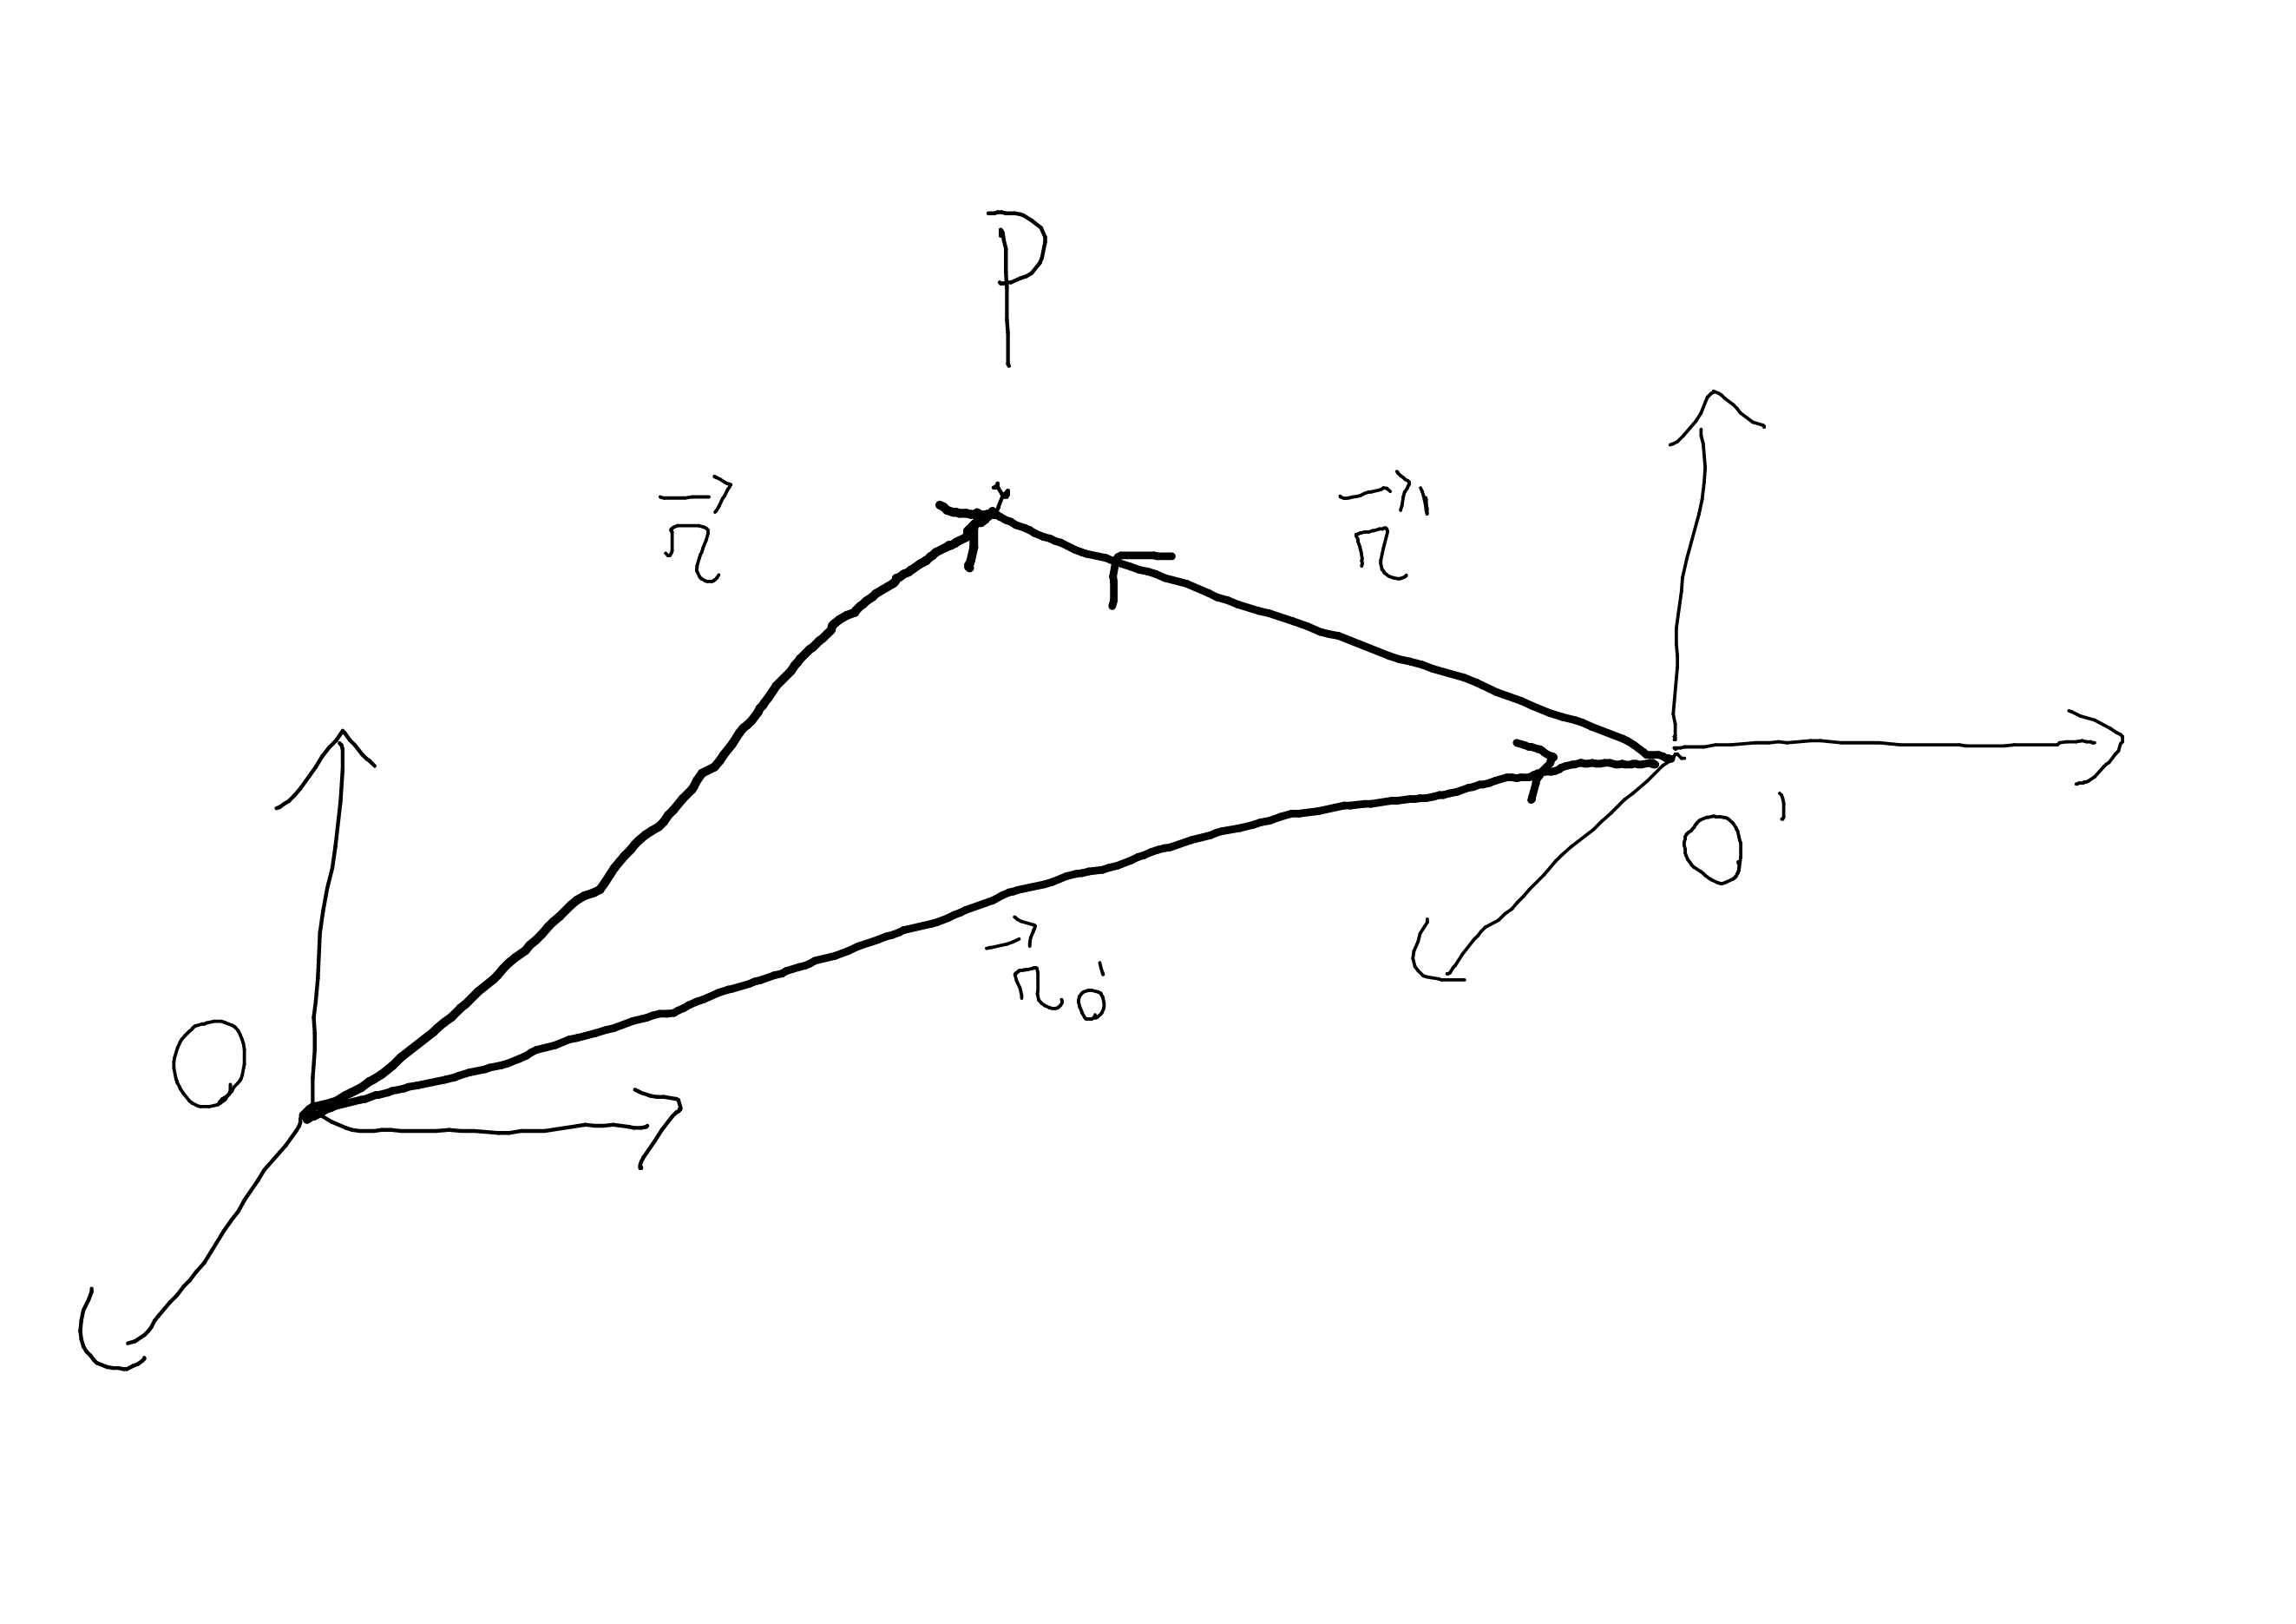
\includegraphics[width=0.4\textwidth]{PosizioneRelativa.png}
\end{figure}
Vettorialmente:
\begin{equation}
    \boxed{\r=\r'+\r_{O'}}
\end{equation}

Derivando rispetto al tempo otteniamo la legge di composizione della velocità, stavolta esplictando in componenti cartesiane:
\begin{equation}
\begin{split}
    \v&=\dv{\r}{t}=\dv{\r'+\r_{O'}}{t}=\\
    &=\dv{\r'}{t}+\dv{\r_{O'}}{t}=\dv{x'\i'+y\j'+z\k'}{t}+\dv{x_{O'}\i+y_{O'}\j+z_{O'}\k}{t}=\\
    &=\Dot{x}'\i'+\Dot{y}'\j'+\Dot{z}'\k'+x\va{\omega}\times\i'+y\va{\omega}\times\j'+z\va{\omega}\times\k'+\v_{O'}=\\
    &=\boxed{\v'+\va{\omega}\times\r'+\v_{O'}}
\end{split}
\end{equation}
Chiamiamo la componente $\v_T(t)=\va{\omega}\times\r'+\v_{O'}$ di \textbf{trascinamento}.\\
\note Abbiamo utilizzato una \hyperlink{vettoreruotante}{proprietà} del vettore ruotante per derivare i vari versori, ottenendo qualcosa del tipo:
\[\dv{\r'}{t}=\v'+\va{\omega}\times\r'\]
Notiamo infatti che tutti e tre i versori di un sistema di riferimento cartesiano devono ruotare secondo lo stesso vettore $\va{\omega}$:
\[\i'\cdot\k'=0\then \dv{(\i'\cdot\k')}{t}=0\then\]
\begin{equation}
\begin{split}
    \then \dv{(\i'\cdot\k')}{t}&=\dv{\i'}{t}\cdot\k'+\i'\cdot\dv{\k'}{t}=\\
    &=(\va{\omega}\times\i')\cdot\k'+\i'\cdot(\va{\omega'}\times\k')=(\i'\times\k')\cdot\va{\omega}+\va{\omega'}(\k'\times\i')=\\
    &=(\i'\times\k')\cdot\va{\omega}-\va{\omega'}(\i'\times\k')=\\
    &=\va{\omega}\cdot(\k'\times\i')-\va{\omega'}(\i'\times\k')=\\
    &=(\va{\omega}-\va{\omega'})(\i'\times\k')=(\va{\omega}-\va{\omega'})\j'=0\iff \boxed{\va{\omega}=\va{\omega'}}    
\end{split}
\end{equation} 


Applichiamo questa osservazione anche alla composizione delle accelerazioni per ridurre i calcoli svolti:
\begin{equation}
\begin{split}
    \a&=\dv{\v}{t}=\dv{\v'+\va{\omega}\times\r'+\v_{O'}}{t}=\\
    &=\a'+\va{\omega}\times\v'+\dv{\va{\omega}\times\r'}{t}+\a_{O'}=\\
    &=\a'+\va{\omega}\times\v'+\Dot{\va{\omega}}\times\r'+\va{\omega}\times\dv{\r'}{t}+\a_{O'}=\\
    &=\a'+\va{\omega}\times\v'+\Dot{\va{\omega}}\times\r'+\va{\omega}\times\left(\v'+\va{\omega}\times\r'\right)+\a_{O'}=\\
    &=\boxed{\a'+\Dot{\va{\omega}}\times\r'+2\va{\omega}\times\v'+\va{\omega}\times\va{\omega}\times\r'}
\end{split}
\end{equation}
Definiamo quindi l'\textbf{accelerazione di trascinamento} $\a_T(t)=\Dot{\va{\omega}}\times\r'+\va{\omega}\times\va{\omega}\times\r'$ e l'\textbf{accelerazione di Coriolis} $\a_c(t)=2\va{\omega}\times\v'$.\\
Abbiamo quindi ottenuto le tre seguenti formule di composizione per posizione, velocità e accelerazione:
\begin{equation}
\boxed{\begin{cases}
    \r=\r'+\r_{O'}\\
    \v=\v'+\va{\omega}\times\r'+\v_{O'}\\
    \a=\a'+\Dot{\va{\omega}}\times\r'+\va{\omega}\times\va{\omega}\times\r'+2\va{\omega}\times\v'
\end{cases}}
\end{equation}

\subsection{Sistemi Inerziali e Non Inerziali}
Ipotesi di fondo per le considerazione della dinamica galileiana-newtoniana è che esiste un riferimento, detto \textbf{sistema di riferimento inerziale}, nel quale sono valide i Principi della Dinamica. In tal caso, risulterà che ogni altro sistema di riferimento che si muove di moto rettilineo uniforme rispetto a questo è anch'esso inerziale, ogni altro sistema si dirà invece \textbf{non inerziale}.\\
Tale sistema si muove di moto accelerato rispetto ad uno inerziale ed è tale che le predizioni fatte dalla dinamica non sono valide, \textit{a meno di correzioni}. Per questo motivo è necessario introdurre, un fattore correttivo all'interno del secondo principio per correttamente predire il moto di un corpo dal punto di vista di un sistema non inerziale, ovviamente questo fattore richiede la conoscenza di fattori "esterni" a tale sistema, che richiedono dati misurati da altri: esso prendo il nome di \textbf{forza apparente}.\\
\paragraph{Le Forze Apparenti}
Il secondo principio applicato in un sistema non inerziale deve tener conto dell'accelerazione del proprio sistema integrando un fattore noto come \textbf{forza apparente} (o \textit{risultante} delle forze apparenti), notando che in un sistema inerziale:
\[\sum\F=m\a=m(\a'+\Dot{\va{\omega}}\times\r'+\va{\omega}\times\va{\omega}\times\r'+2\va{\omega}\times\v')\]
Mentre le forze \textit{reali} percepite dal sistema saranno sempre $\sum\F$, l'accelerazione misurata sarà invece $\a'$, quindi spostiamo al primo membro l'accelerazione di trascinamento e di Coriolis, questa forza prende il nome di \textbf{forza apparente}:
\[\sum\F-m(\Dot{\va{\omega}}\times\r'+\va{\omega}\times\va{\omega}\times\r'+2\va{\omega}\times\v')=\sum\F+\F_A=m\a'\quad\quad \boxed{\F_A=-m(\Dot{\va{\omega}}\times\r'+\va{\omega}\times\va{\omega}\times\r'+2\va{\omega}\times\v')}\]

\chapter{Conseguenze dei Principi della Dinamica}
Come già detto, i principi della dinamica non sono sufficienti per descrivere completamente il moto di un corpo, ma sono necessarie ulteriori considerazioni capaci di ottenere risultati più generali.
\section{Quantità di Moto e Impulso}
Introduciamo la grandezza \textbf{quantità di moto}, definita dalla seguente formula:
\begin{equation}
    \p=m\v
\end{equation}
Conseguenza quasi immediata è il \textbf{Teorema dell'Impulso}:
\begin{thm}[Teorema dell'Impulso]
\begin{equation}
\begin{split}
    \va{I}=\int_{t_1}^{t_2}\F(t)\dif t=\\
    &=\int_{t_1}^{t_2}m\a\dif t=\\
    &=\int_{t_1}^{t_2}m\dv{\v}{t}\dif t=\\
    &=\int_{t_1}^{t_2}\dv{\p}{t}\dif t=\\
    &=\int_{t_1}^{t_2}\dif\p=\p(t_2)-\p(t_1)=\Delta\p
\end{split}
\end{equation}
Viceversa si ottiene:
\begin{equation}
    \dv{\p}{t}=\dv{m\v}{t}=m\dv{\v}{t}=m\a=\F\then \boxed{\F=\dv{\p}{t}}
\end{equation}
\end{thm}
Questo teorema rappresenta una generalizzazione del secondo principio della dinamica, che ci conduce a un altra formulazione del principio d'inerzia considerando un corpo la cui risultante delle forze è nulla:
\begin{equation}
    \dv{\p}{t}=0\then\boxed{\p=cost}
\end{equation}
Il teorema dell'impulso fornisce anche un'importante risultato per l'analisi degli \textbf{urti}, ossia \textit{fenomeni d'interazione tra due o più corpi dotati di una durata limitata}. Un urto pertanto può essere anche l'avvicinamento di un asteroide al Sole, non solo il contatto di due corpi in velocità.\\
Tuttavia gli urti di breve durata sono particolarmente interessanti e presentano caratteristiche che ne rendono facile lo studio. 
\paragraph{Urti di Breve Durata}
Tutti gli urti di breve durata capaci di modificare significativamente la quantità di moto dei corpi coinvolti coinvolgono forze d'interazione interne, tali che valgono le seguenti relazioni (per due corpi) durante il tempo d'interazione:
\begin{equation}
\begin{cases}
    m_1\a_1=\f_{12}+\F_1^{(e)}\\
    m_2\a_2=\f_{21}+\F_2^{(e)}=-\f_{12}+\F_2^{(e)}
\end{cases}\then m_1\a_1+m_2\a_2=\F_1^{(e)}+\F_2^{(e)}\neq0\then\dv{\P}{t}\neq0
\end{equation}
Pertanto le variazioni degli impulsi diventano:
\begin{equation}
\I_{12}+\I_{21}=0\quad
\begin{cases}
    \Delta\p_1=\I_{12}+\I_1^{(e)}\\
    \Delta\p_2=\I_{21}+\I_2^{(e)}
\end{cases}
\end{equation}
Siccome le interazioni interne sono molto brevi ma molto intense risulta:
\begin{figure}[H]
    \centering
    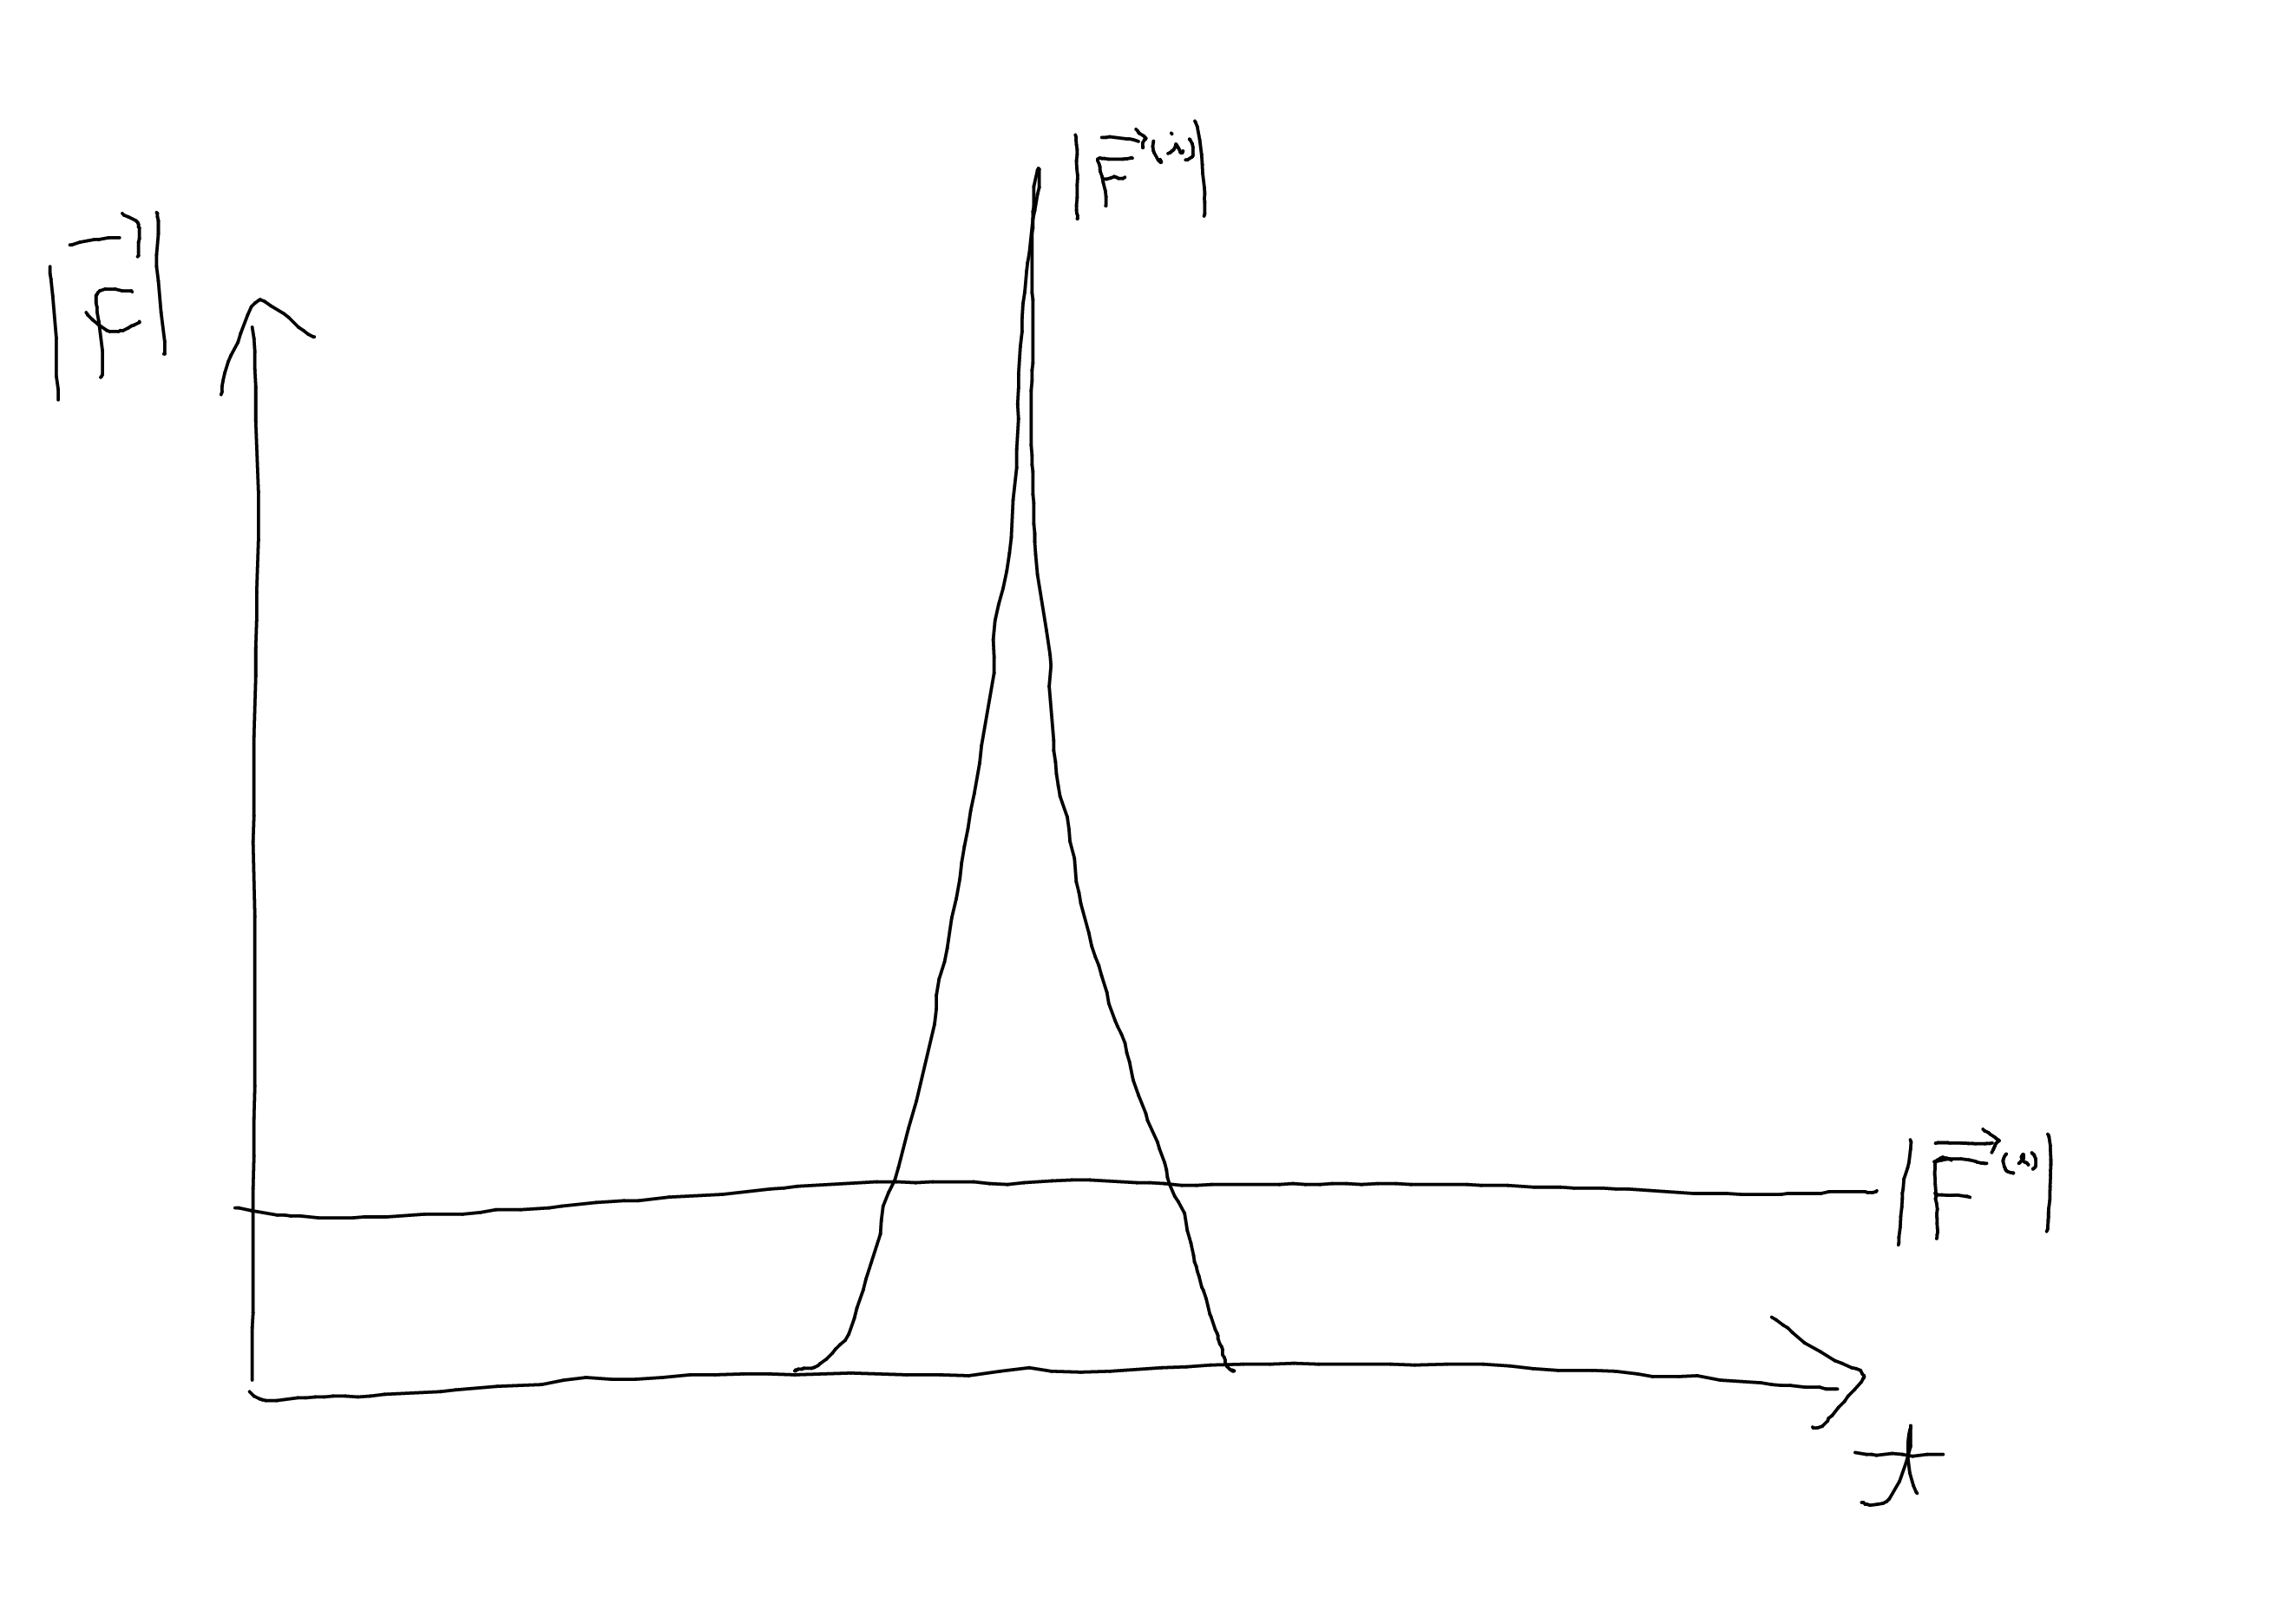
\includegraphics[width=0.5\textwidth]{UrtiBrevi.png}
\end{figure}
Da cui risulta che:
\begin{equation}
\begin{cases}
    |\I_{12}|\gg|\I_1^{(e)}|\\
    |\I_{21}|\gg|\I_2^{(e)}
\end{cases}\then
\begin{cases}
    \Delta\p_1\approx\I_{12}\\
    \Delta\p_2\approx\I_{21}
\end{cases}\then \Delta\P\approx0
\end{equation}
Le categorie di urti che possono essere studiate più facilmente sono due: urti \textbf{elastici} e \textbf{completamente anelastici}.
\paragraph{Urti Elastici}
Gli urti elastici sono caratterizzati da due leggi di conservazioni:
\begin{align}
    \Delta\P=0\\
    \Delta K=0
\end{align}
\note La quantità di moto si conserva come vettore solo se le forze esterne non presentano carattere impulsivo, come nel caso delle \textit{forze vincolari}. L'energia cinetica si conserva invece se c'è assenza di forze dissipative non c'è variazione significativa della posizione verticale (tale da cambiare l'energia potenziale dovuta al campo gravitazionale). 
\paragraph{Urti Completamente Anelastici}
Negli urti completamente anelastici l'unica grandezza che si conserva (nelle stesse ipotesi degli urti elastici) è la quantità di moto, mentre si conserva il minimo dell'energia cinetica, in quanto i due corpi iniziano a muoversi insieme con la stessa velocità, fornendo quindi l'informazione necessaria a sostituire quella data dalla conservazione dell'energia cinetica. 


\section{Lavoro ed Energia}
Definiamo la \textbf{potenza istantanea} di una forza:
\begin{equation}
    W(t)=\F(t)\cdot\v(t)
\end{equation}
Da cui possiamo definire il \textbf{lavoro} di una forza tra due istanti:
\begin{equation}
    L(t_1,t_2)=\int_{t_1}^{t_2}W(t)\dif t=\int_{t_1}^{t_2}\F(t)\cdot\v(t)\dif t
\end{equation}
Quest'espressione è equivalente alla seguente notando che:
\begin{equation}
    L=\int_{t_1}^{t_2}\F(t)\cdot\v(t)\dif t=\int_{t_1}^{t_2}\F(t)\cdot\dv{\r(t)}{t}\dif t=\int_{\r_1}^{\r_2}\F(\r)\cdot\dif\r
\end{equation}
Ossia possiamo calcolare il lavoro compiuto da una forza tra due istanti considerando la forza come funzione della posizione $\F(\r)$ e calcolare il lavoro tra due posizioni (lungo uno spostamento). Questa definizione presenta tuttavia alcune problematiche di tipo matematico in quanto richiede la conoscenza degli integrali di linea (nel caso generale), mentre la prima si limitava agli integrali di Riemann. \hypertarget{ForzeVive}{Possiamo ottenere alcuni risultati considerando già la prima espressione.}
\begin{thm}[Teorema dell'Energia Cinetica]
\begin{equation}
\begin{split}
    W(t)&=\F(t)\cdot\v(t)=\\
    &=m\a(t)\cdot\v(t)=\\
    &=m\dv{\v(t)}{t}\v(t)=\\
    &=m\frac{2}{2}\dv{\v}{t}\cdot\v=\\
    &=\frac{1}{2}m\left(2\dv{\v}{t}\cdot\v\right)=\\
    &=\frac{1}{2}m\dv{\v\cdot\v}{t}=\\
    &=\frac{1}{2}m\dv{v^2}{t}=\\
    &=\dv{t}\left(\frac{1}{2}mv^2\right)=\boxed{\dv{K}{t}}
\end{split}
\end{equation}
Definiamo quindi la grandezza \textbf{energia cinetica} come l'oggetto $K=\frac{1}{2}mv^2$ e tale che:
\[W(t)=\dv{K}{t}\]
Immediata conseguente è sul lavoro:
\[L(t_1,t_2)=\int_{t_1}^{t_2}W(t)\dif t=\int_{t_1}^{t_2}\dv{K}{t}\dif t=K(t_2)-K(t_1))=\Delta K\]
Ossia una forza che agisce in un certo intervallo di tempo (o lungo un certo spostamento) determina una variazione dell'energia cinetica:
\[\boxed{\L=\Delta K}\]
\end{thm}
\paragraph{Lavoro come Integrale di Linea}
Considerare il lavoro di una forza come integrale di linea della forza permette numerosi vantaggi; inoltre facendo alcune conservazioni sul prodotto scalare possiamo anche considerare l'integrale di linea come un integrale di Riemann.\\
Schematizzando il prodotto scalare $\F(t)\cdot\dif\r$ otteniamo la seguente figura:
\begin{figure}[H]
    \centering
    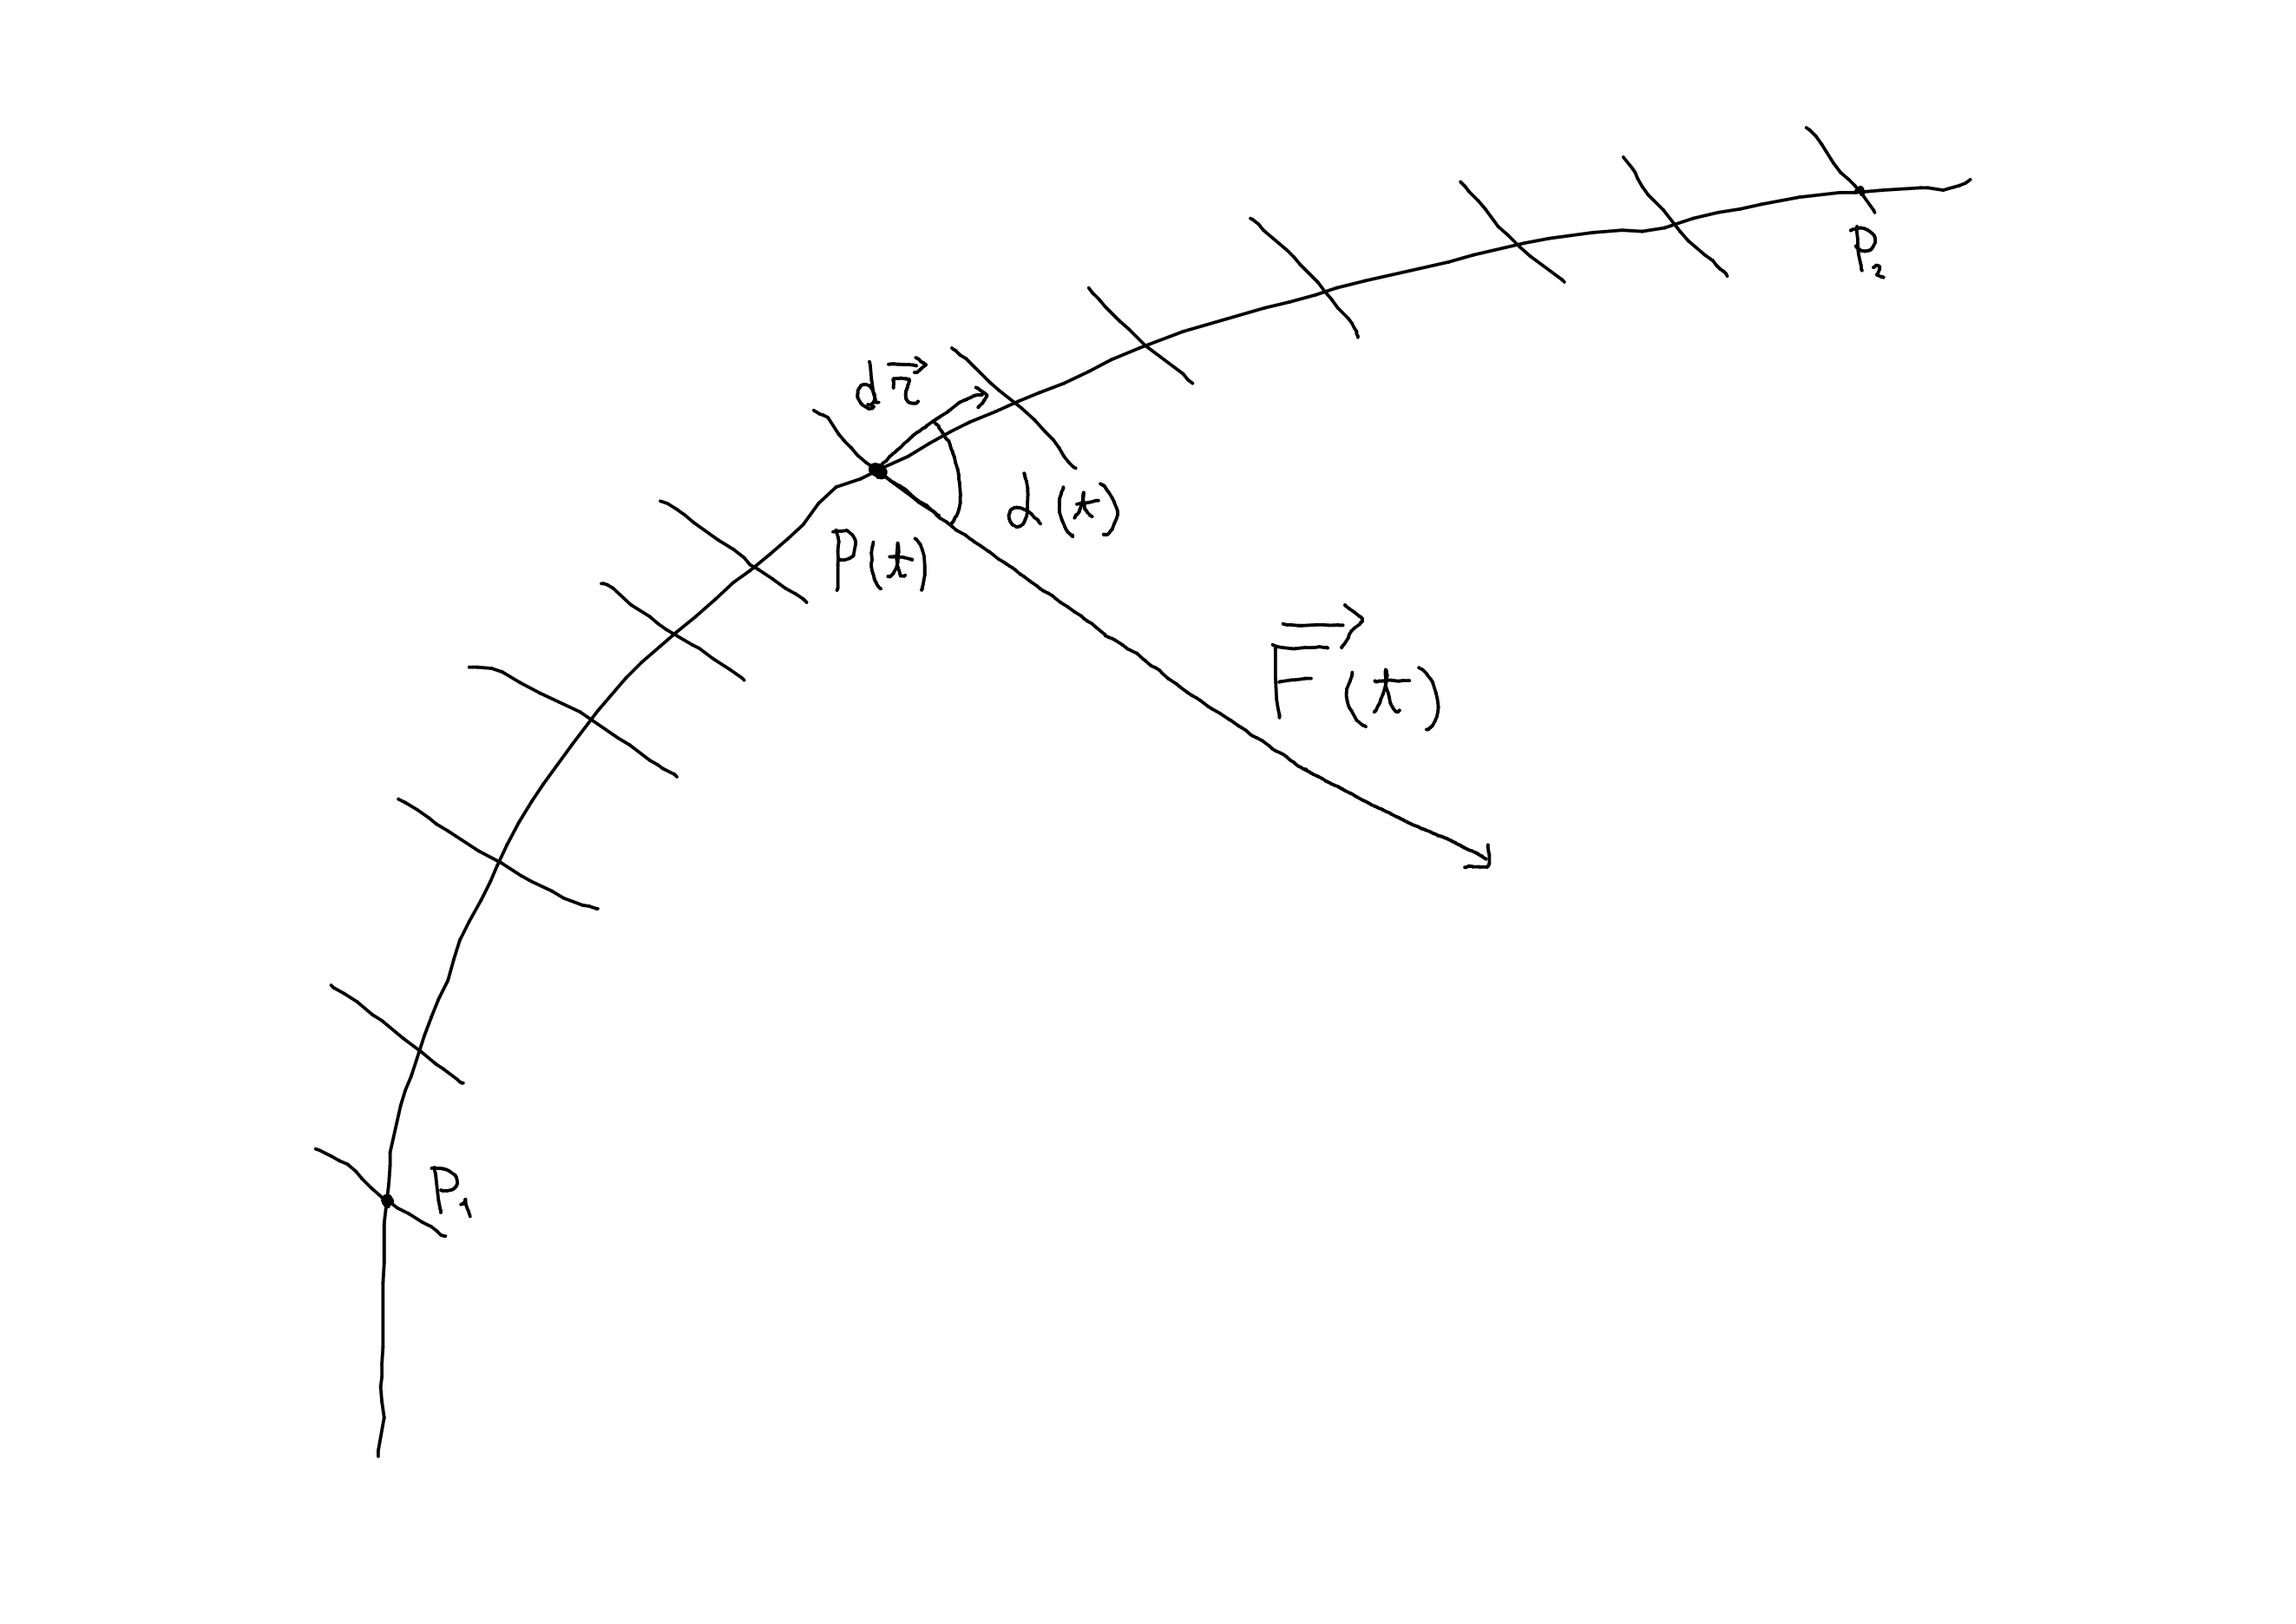
\includegraphics[width=0.5\textwidth]{IntegraleLinea.png}
\end{figure}
Dove $P(t)$ è la posizione al tempo t e ad $\alpha(t)$ è l'angolo tra lo spostamento infinitesimo e la forza applicata.\\
Ossia possiamo esplicitare come segue:
\begin{equation}
\begin{split}
    \F(t)\cdot\dif\r&=\abs{\F}\abs{\dif\r}\cos\alpha(t)=\\
    &=\abs{\F}\dif s\cos\alpha(t)=\\
    &=\abs{\F}\cos\alpha(s)\dif s\then\\
    &\then\boxed{L=\int_{s_1}^{s_2}\abs{\F(s)}\cos\alpha(s)\dif s}
\end{split}
\end{equation}
Notiamo che il modulo dello spostamento coincide con il valore di una variazione infinitesima dell'ascissa curvilinea, che essendo funzione del tempo può essere invertita in modo tale da rendere il modulo della forza e l'angolo tra $\F$ e $\dif\r$ entrambe funzioni dell'ascissa curvilinea. Abbiamo quindi ottenuto un integrale di Riemann, come volevasi dimostrare.\\
Un caso tipico in cui considerare il lavoro come integrale di linea risulta particolarmente utile è quello una forza agisce su un corpo in modo che la direzione della forza e la direzione dello spostamento siano tra loro perpendicolari istante per istante, questo è ad esempio il caso della tensione, che non compie lavoro su un pendolo in moto:
\begin{equation}
    \va{\tau}\perp\dif\r\then\va{\tau}\cdot\dif\r=0\then \delta L=\va{\tau}\cdot\dif\r=0\then \boxed{L=0}
\end{equation}
\begin{figure}[H]
    \centering
    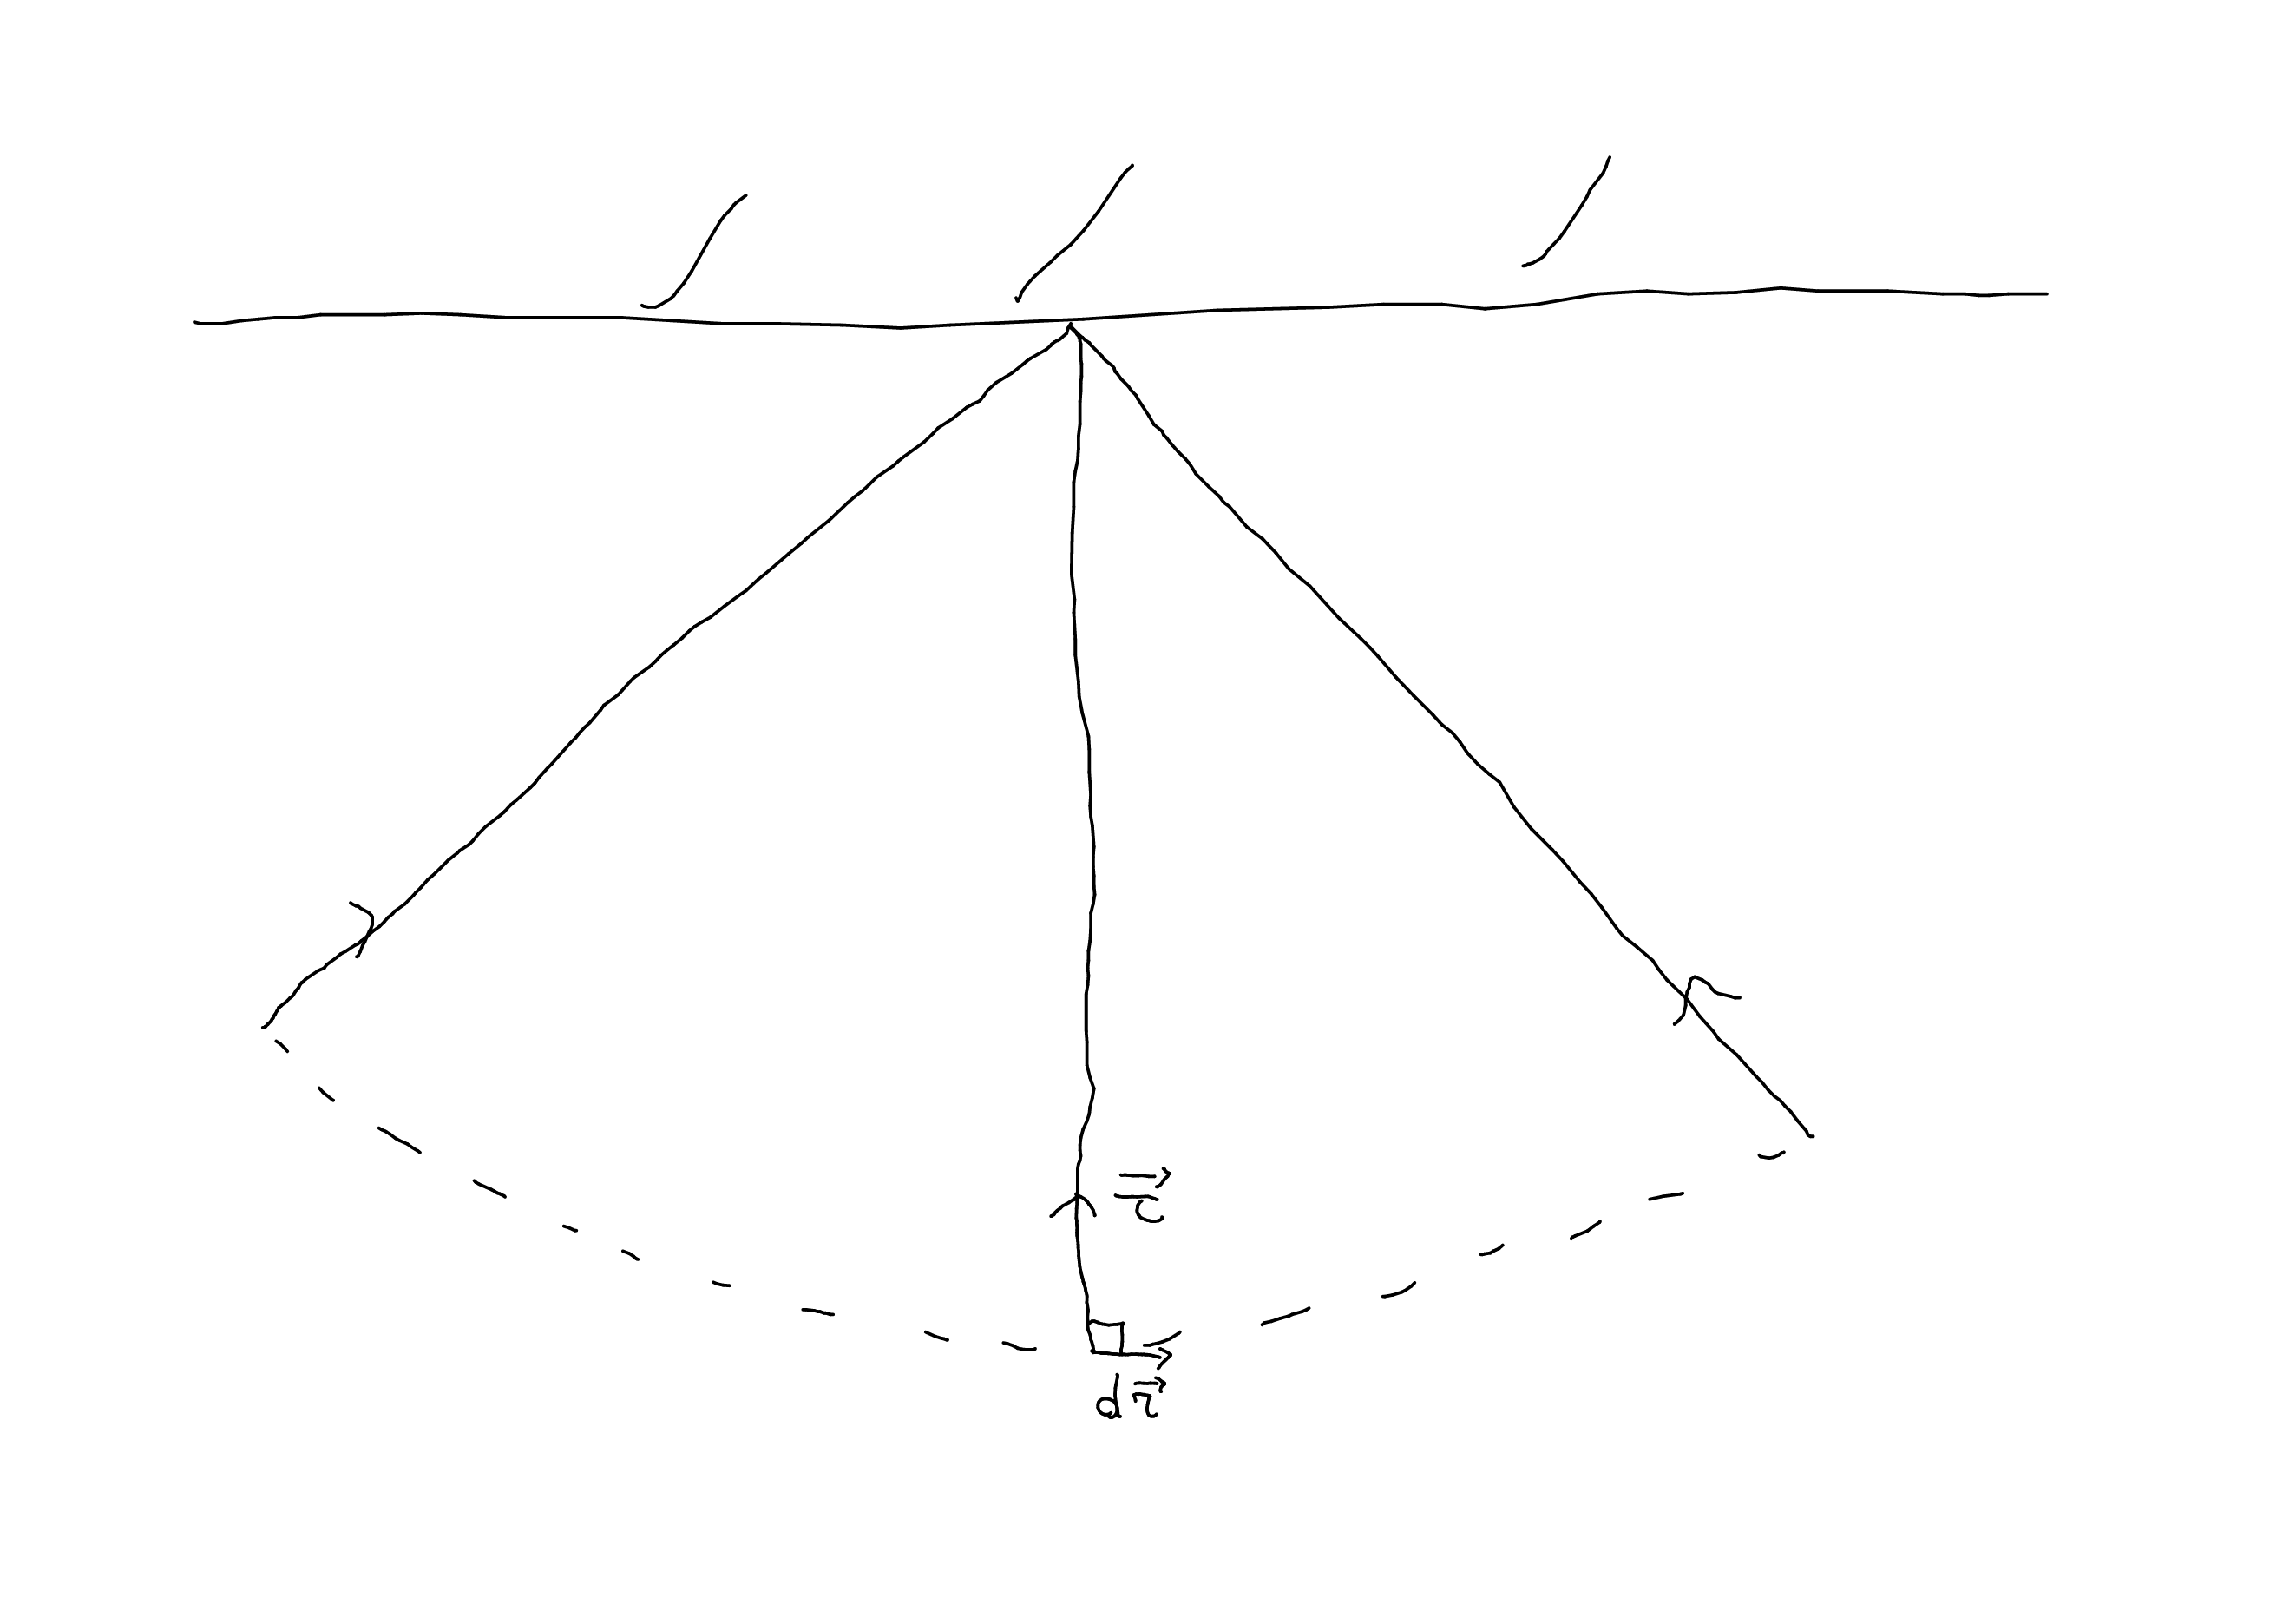
\includegraphics[width=0.5\textwidth]{LavoroIntLinea.png}
\end{figure}

\section{I Campi di Forza}
Un \textbf{campo di forza} è una certa funzione $\F(\r)$ che associa ad ogni punto appartenente ad una certa parte di spazio una forza $\F$:
\begin{figure}[H]
    \centering
    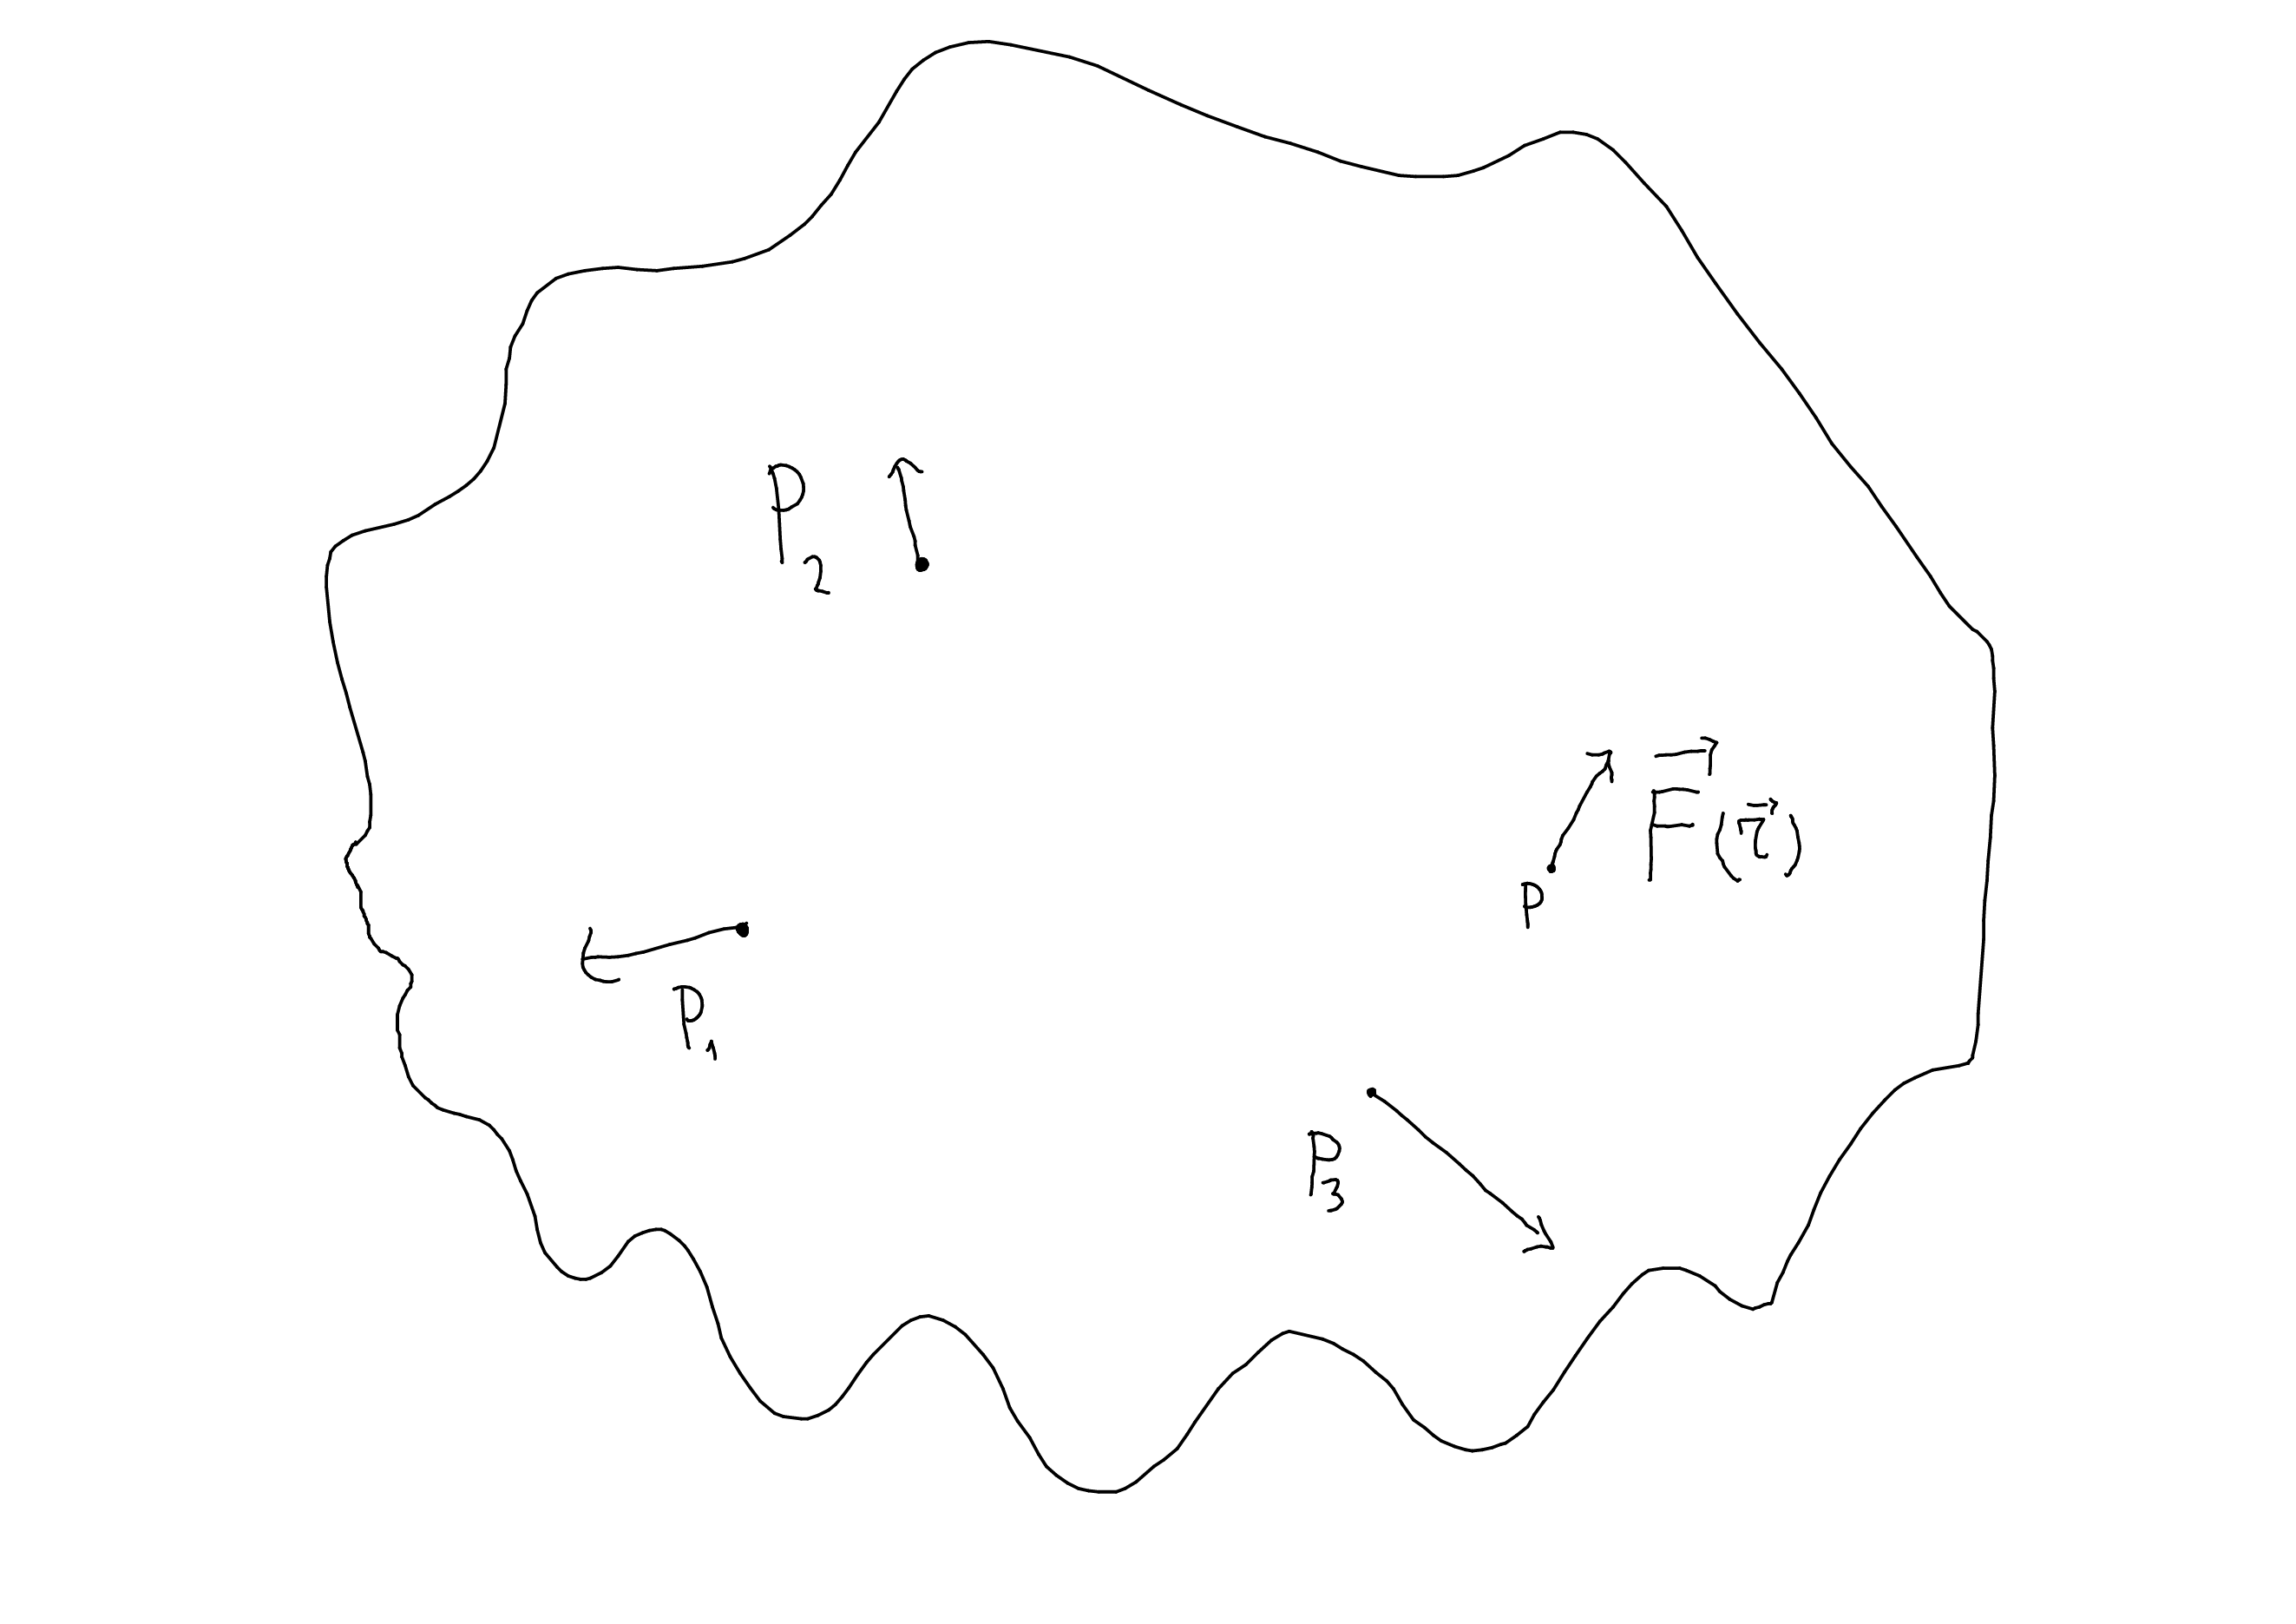
\includegraphics[width=0.5\textwidth]{CampodiForze.png}
\end{figure}
Un campo di forze si dice \textbf{uniforme} se associata ad ogni punto dello spazio lo stesso vettore (come la forza-peso) e \textbf{costante} se non varia nel tempo. Notiamo che in generale il lavoro tra due posizioni dipende dalla traiettoria (spostamento) e non solo dalle posizioni iniziali e finali:
\begin{figure}[H]
    \centering
    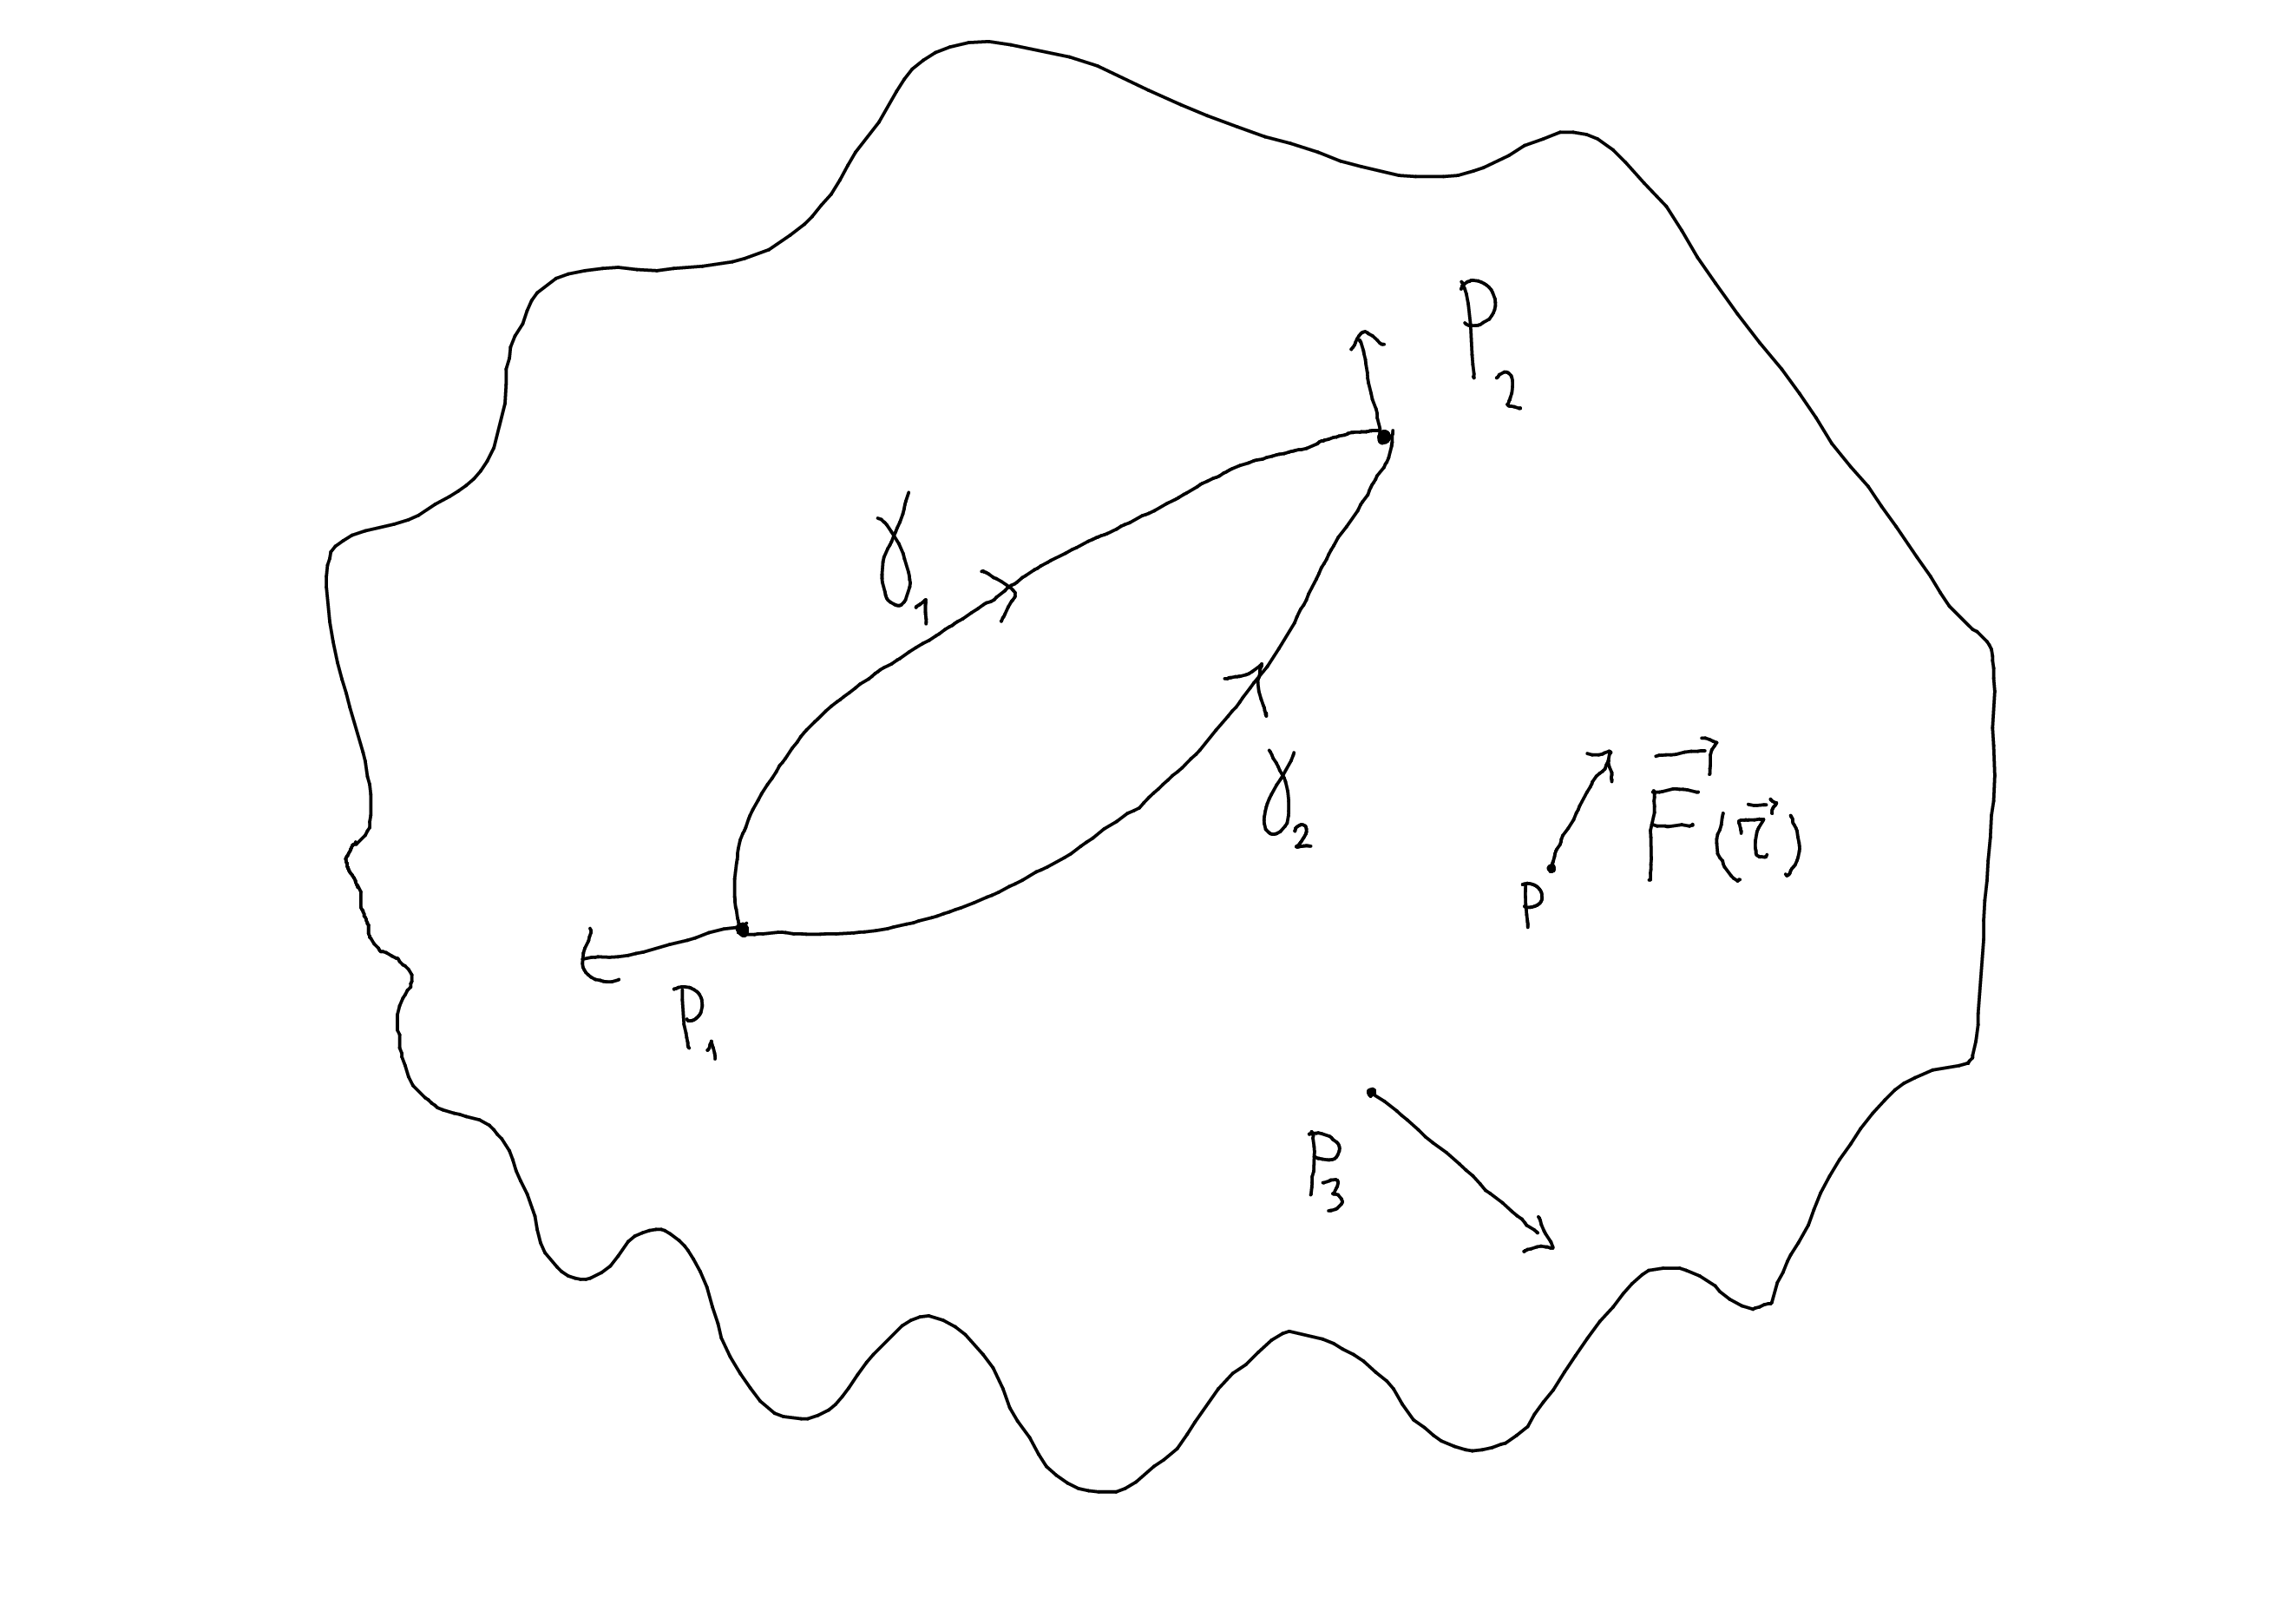
\includegraphics[width=0.5\textwidth]{TraiettorieCampiForza.png}
\end{figure}
\[L_1={}_{\gamma_1}\int_{P_1}^{P_2}\F(\r)\dif\r\neq{}_{\gamma_2}\int_{P_1}^{P_2}\F(\r)\dif\r=L_2\]
\paragraph{Campi di Forza Conservativi}
Un campo di forza di dice \textbf{conservativo}, se il lavoro tra due posizioni è lo stesso per ogni traiettoria, ossia è \textbf{indipendente dalla traiettoria}. Cerchiamo ora un modo di caratterizzare questa proprietà matematicamente, facendo considerazioni sugli integrali:
\[{}_{\gamma_1}\int_{P_1}^{P_2}\F(\r)\dif\r={}_{\gamma_2}\int_{P_1}^{P_2}\F(\r)\dif\r=-{}_{\gamma_2}\int_{P_2}^{P_1}\F(\r)\dif\r\then {}_{\gamma_1}\int_{P_1}^{P_2}\F(\r)\dif\r+{}_{\gamma_2}\int_{P_2}^{P_1}\F(\r)\dif\r=0\then\boxed{\oint\F(\r)\dif\r=0}\]
Ossia l'\textbf{integrale di linea di una forza lungo un percorso chiuso è nullo} è una proprietà caratterizzante dei campi conservativi. 
\subsection{Energia Potenziale}
Usando la proprietà appena descritta possiamo definire una funzione $V$ tale che dipenda solo dai punti di inizio e di arrivo:
\[V(P_1,P_2)=\int_{P_1}^{P_2}\F(\r)\dif\r\]
Fissando un certo punto arbitrario $P$ tra $P_1$ e $P_2$ otteniamo per la proprietà additiva degli integrali:
\[\int_{P_1}^{P_2}\F(\r)\dif\r=\int_{P_1}^{P}\F(\r)\dif\r+\int_{P}^{P_2}\F(\r)\dif\r\quad\quad\int_{P_1}^{P_2}\F(\r)\dif\r=-\int_{P_2}^{P_1}\F(\r)\dif\r\]
\begin{figure}[H]
    \centering
    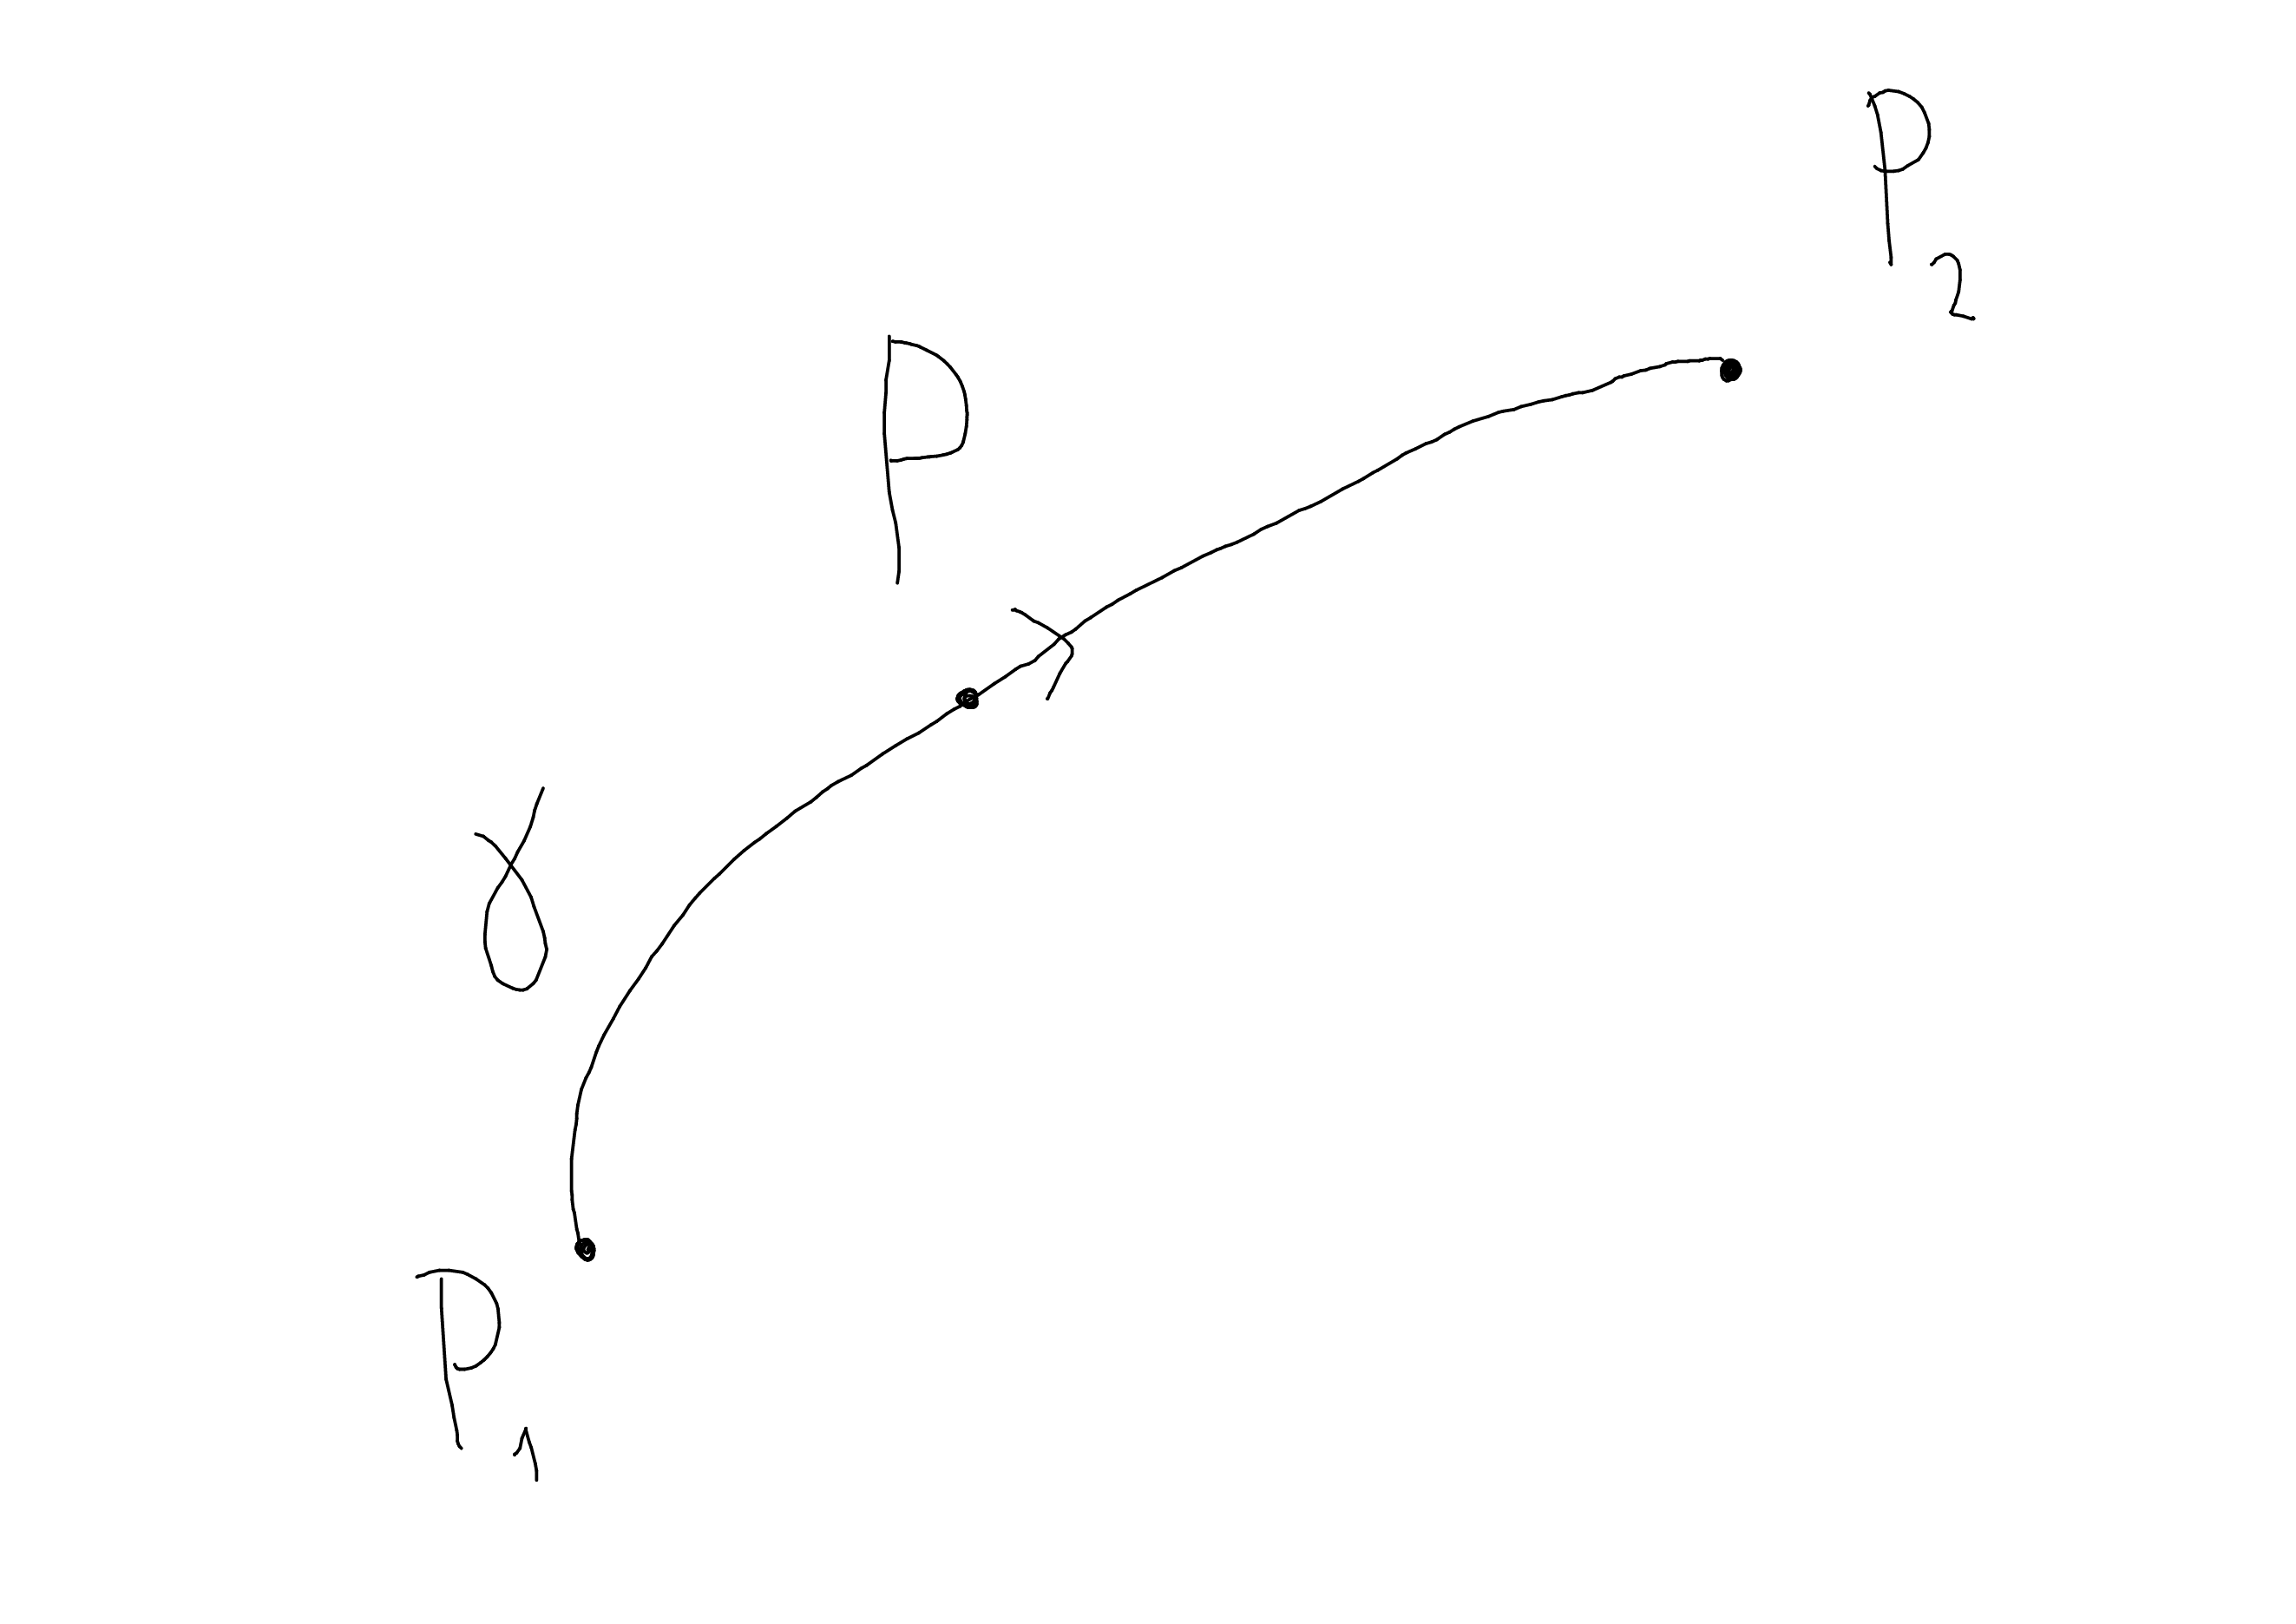
\includegraphics[width=0.5\textwidth]{Potenziale.png}
\end{figure}
Quindi varrà anche:
\[V(P_1,P_2)=V(P_1,P)+V(P,P_2)=-V(P,P_1)+V(P_2,P)\]
Ma siccome P è un punto arbitrario allora $V(P_1,P)$ e $V(P,P_2)$ in realtà sono funzioni solamente di $P_1$ e $P_2$ quindi possiamo scrivere:
\[V(P_1,P_2)=-V(P,P_1)+V(P_2,P)=-U(P_1)+U(P_2)=\boxed{U(P_2)-U(P_1)}\]
Definiamo questa funzione scalare $U$ \textbf{energia potenziale} del campo conservativo di una forza. Inoltre, così come vale la proprietà additiva per il lavoro (in tale caso puramente conservativo), così vale per le variazioni di energie potenziale:
\begin{align*}
    L_T^{(cons)}=-\Delta U\\
    L_1+L_2=-\Delta U\\
    -\Delta U_1-\Delta U_2=-\Delta U\\
    [U_1(P_1)-U_1(P_2)]+[U_2(P_1)-U_2(P_2)]=U(P_1)-U(P_2)\\
    [U_1(P_1)+U_2(P_2)]-[U_1(P_2)+U_2(P_2)]=U(P_1)-U(P_2)\then\\
    \then \boxed{U_1+U_2=U}
\end{align*}
E in generale:
\[\sum_i^nL_i^C=-\Delta\left(\sum_i^nU_i\right)\]
Inoltre, avendo definito l'energia potenziale come variazione, in realtà essa è definita per un punto a meno di una costante:
\[U(P)=\int_{P_0}^P\F(\r)\dif\r+cost\]
\subparagraph{Il Gradiente dell'Energia Potenziale}
Considerando la variazione infinitesima di energia potenziale $\dif U$, può essere scritta come segue:
\[\dif U=\pdv{U}{x}\dif x+\pdv{U}{z}\dif z+\pdv{U}{z}\dif z\]
Ossia $\dif U$ è un \textbf{differenziale}, in quanto può essere scritto come combinazione lineare dei differenziali $\dif x$ moltiplicati per le derivate parziali $\pdv{U}{x}$,\\
Mentre il lavoro infinitesimo $\delta L$ in generale questo si può scrivere come:
\[\delta L=\F(\r)\dif\r=F_x(\r)\dif x+F_y(\r)\dif y+F_z(\r)\dif z\]
Notiamo che il lavoro \textit{non} può essere scritto allo stesso modo dell'energia potenziale, seppur ottenendo una combinazione lineare dei $\dif x,\dif y,\dif z$ e viene pertanto chiamato \textbf{forma differenziale}. Nel caso in cui $\F(\r)$ sia un campo di forze conservativo allora possiamo scrivere:
\begin{align*}
    \delta L=-\dif U\\
    F_x(\r)\dif x+F_y(\r)\dif y+F_z(\r)\dif z=\pdv{U}{x}\dif x+\pdv{U}{z}\dif z+\pdv{U}{z}\dif z
\end{align*}
Ma ciò è vero \textit{se e solo se}:
\begin{equation}
\begin{cases}
    F_x=-\pdv{U}{x}\\
    F_y=-\pdv{U}{y}\\
    F_z=-\pdv{U}{z}
\end{cases}
\end{equation}
Oppure in scrittura vettoriale possiamo introdurre il \textbf{gradiente} del campo scalare U:
\begin{equation}
\F=
\begin{pmatrix}
F_x\\F_y\\F_z
\end{pmatrix}=
-\begin{pmatrix}
\pdv{U}{x}\\\pdv{U}{y}\pdv{U}{z}
\end{pmatrix}=-grad U=-\nabla U
\then\boxed{\F=-\nabla U}
\end{equation}
\paragraph{Energia Meccanica}
Combinando le informazioni del \hyperlink{ForzeVive}{Teorema dell'Energia Cinetica} e dei campi conservativi possiamo definire, una nuova grandezza, nota come \textbf{energia meccanica} $E$:
\begin{align*}
    L=\Delta K\\
    L^C+L^{NC}=\Delta K\\
    -\Delta U+L^{NC}=\Delta K\\
    L^{NC}=\Delta K+\Delta U\\
    L^{NC}=\Delta (K+U)\\
    \boxed{L^{NC}=\Delta E}
\end{align*}
Ossia l'energia meccanica si definisce come la somma di energia potenziale e cinetica di un sistema $E=K+U$. Queste osservazioni formano il \textbf{Teorema Generale dell'Energia Meccanica}, che afferma che una variazione di energia meccanica corrisponde al lavoro di forze non-conservative, anche note come \textbf{dissipative}.
\paragraph{Equilibri}
Studiamo il campo vettoriale (unidimensionale) dovuto alla deformazione di una molla fissata per un estremo. Scegliendo un sistema di riferimento nella posizione di riposo con asse x otteniamo:
\[F(x)=-kx\]
Calcoliamo il lavoro e verifichiamo se può essere espresso come differenza di una funzione nei punti di inizio e di arrivo:
\begin{equation}
\begin{split}
    L&=\int_{x_1}^{x_2}F(x)\dif x=\\
    &=\int_{x_1}^{x_2}-kx\dif x=\\
    &=-k\int_{x_1}^{x_2}x\dif x=\\
    &=-k\frac{1}{2}\eval{x^2}_{x_1}^{x_2}=\\
    &=-\frac{1}{2}k(x_2^2-x_1^2)=\\
    &=\frac{1}{2}kx_1^2-\frac{1}{2}kx_2^2=\boxed{U(x_1)-U(x_2)}
\end{split}
\end{equation}
Otteniamo quindi un grafico del tipo:
\begin{figure}[H]
    \centering
    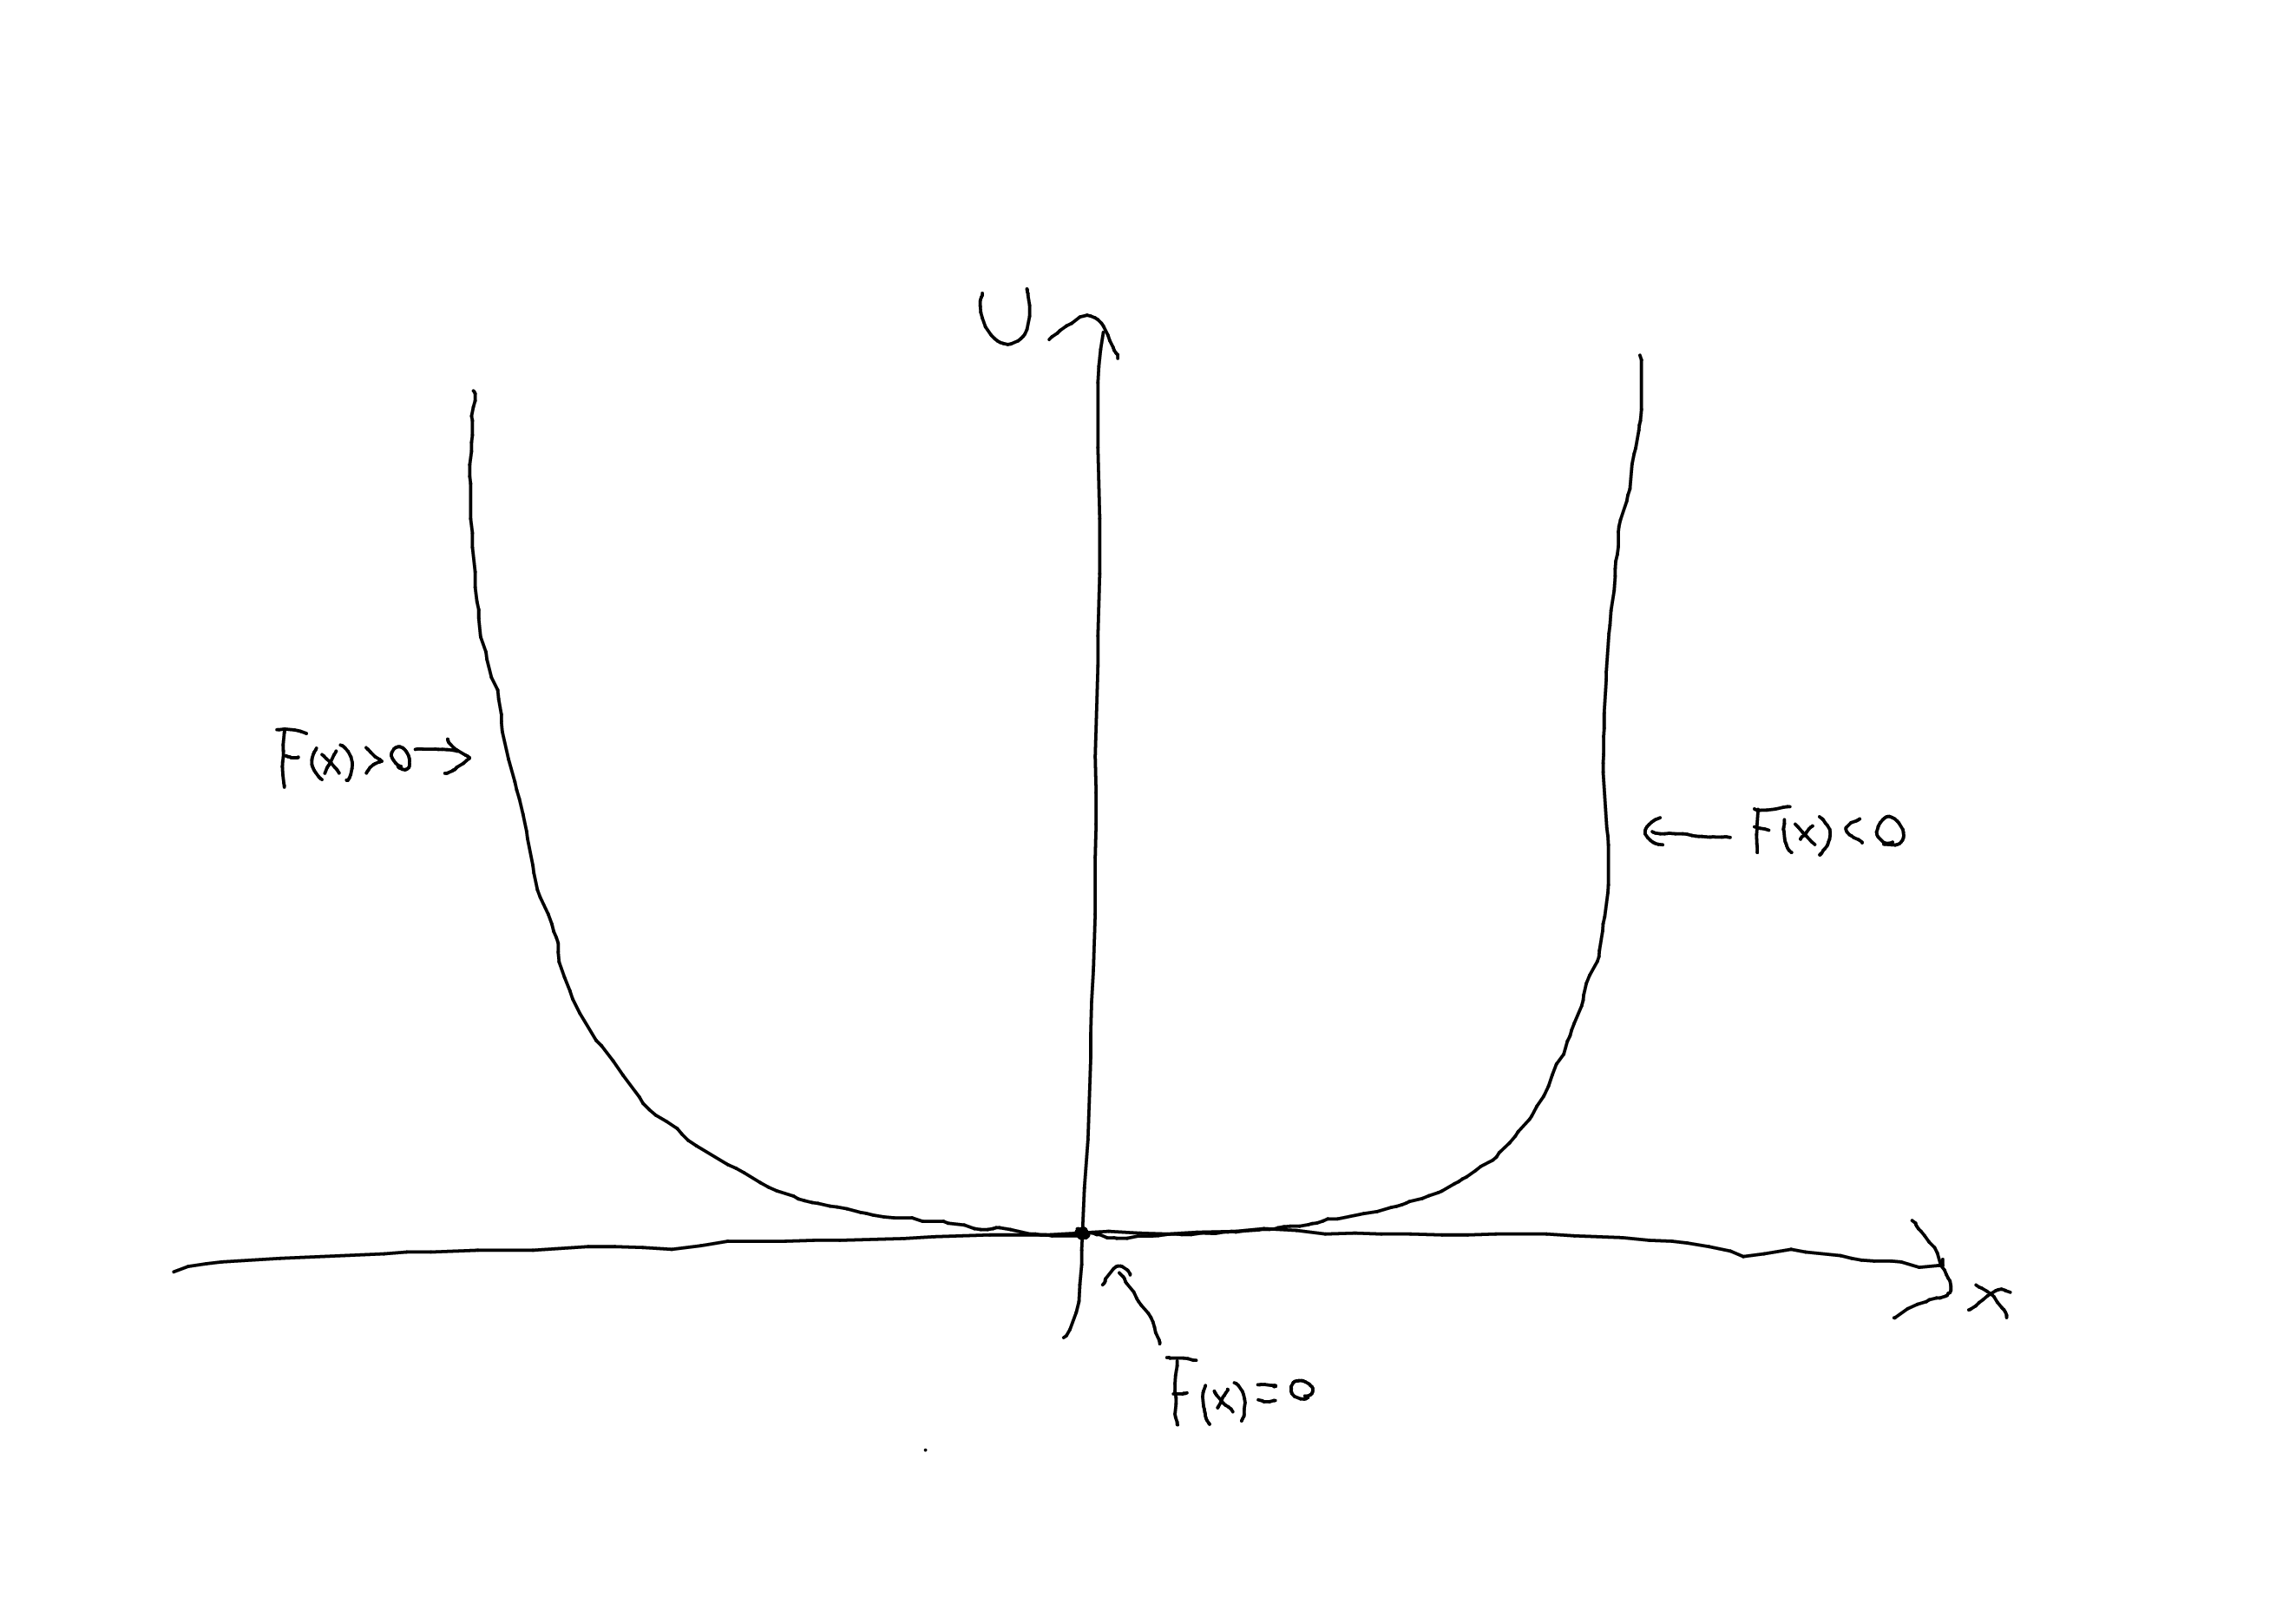
\includegraphics[width=0.5\textwidth]{EnergiaMolla.png}
\end{figure}
Notiamo che il punto più in bassa del grafico è il punto a cui tende spontaneamente la molla, ossia quello con deformazione nulla (la posizione di riposo), un punto del genere prende il nome di \textbf{punto di equilibrio}. In generale ogni campo di forza ha punti di equilibrio a cui tende il corpo soggetto alla forza:
\begin{figure}[H]
    \centering
    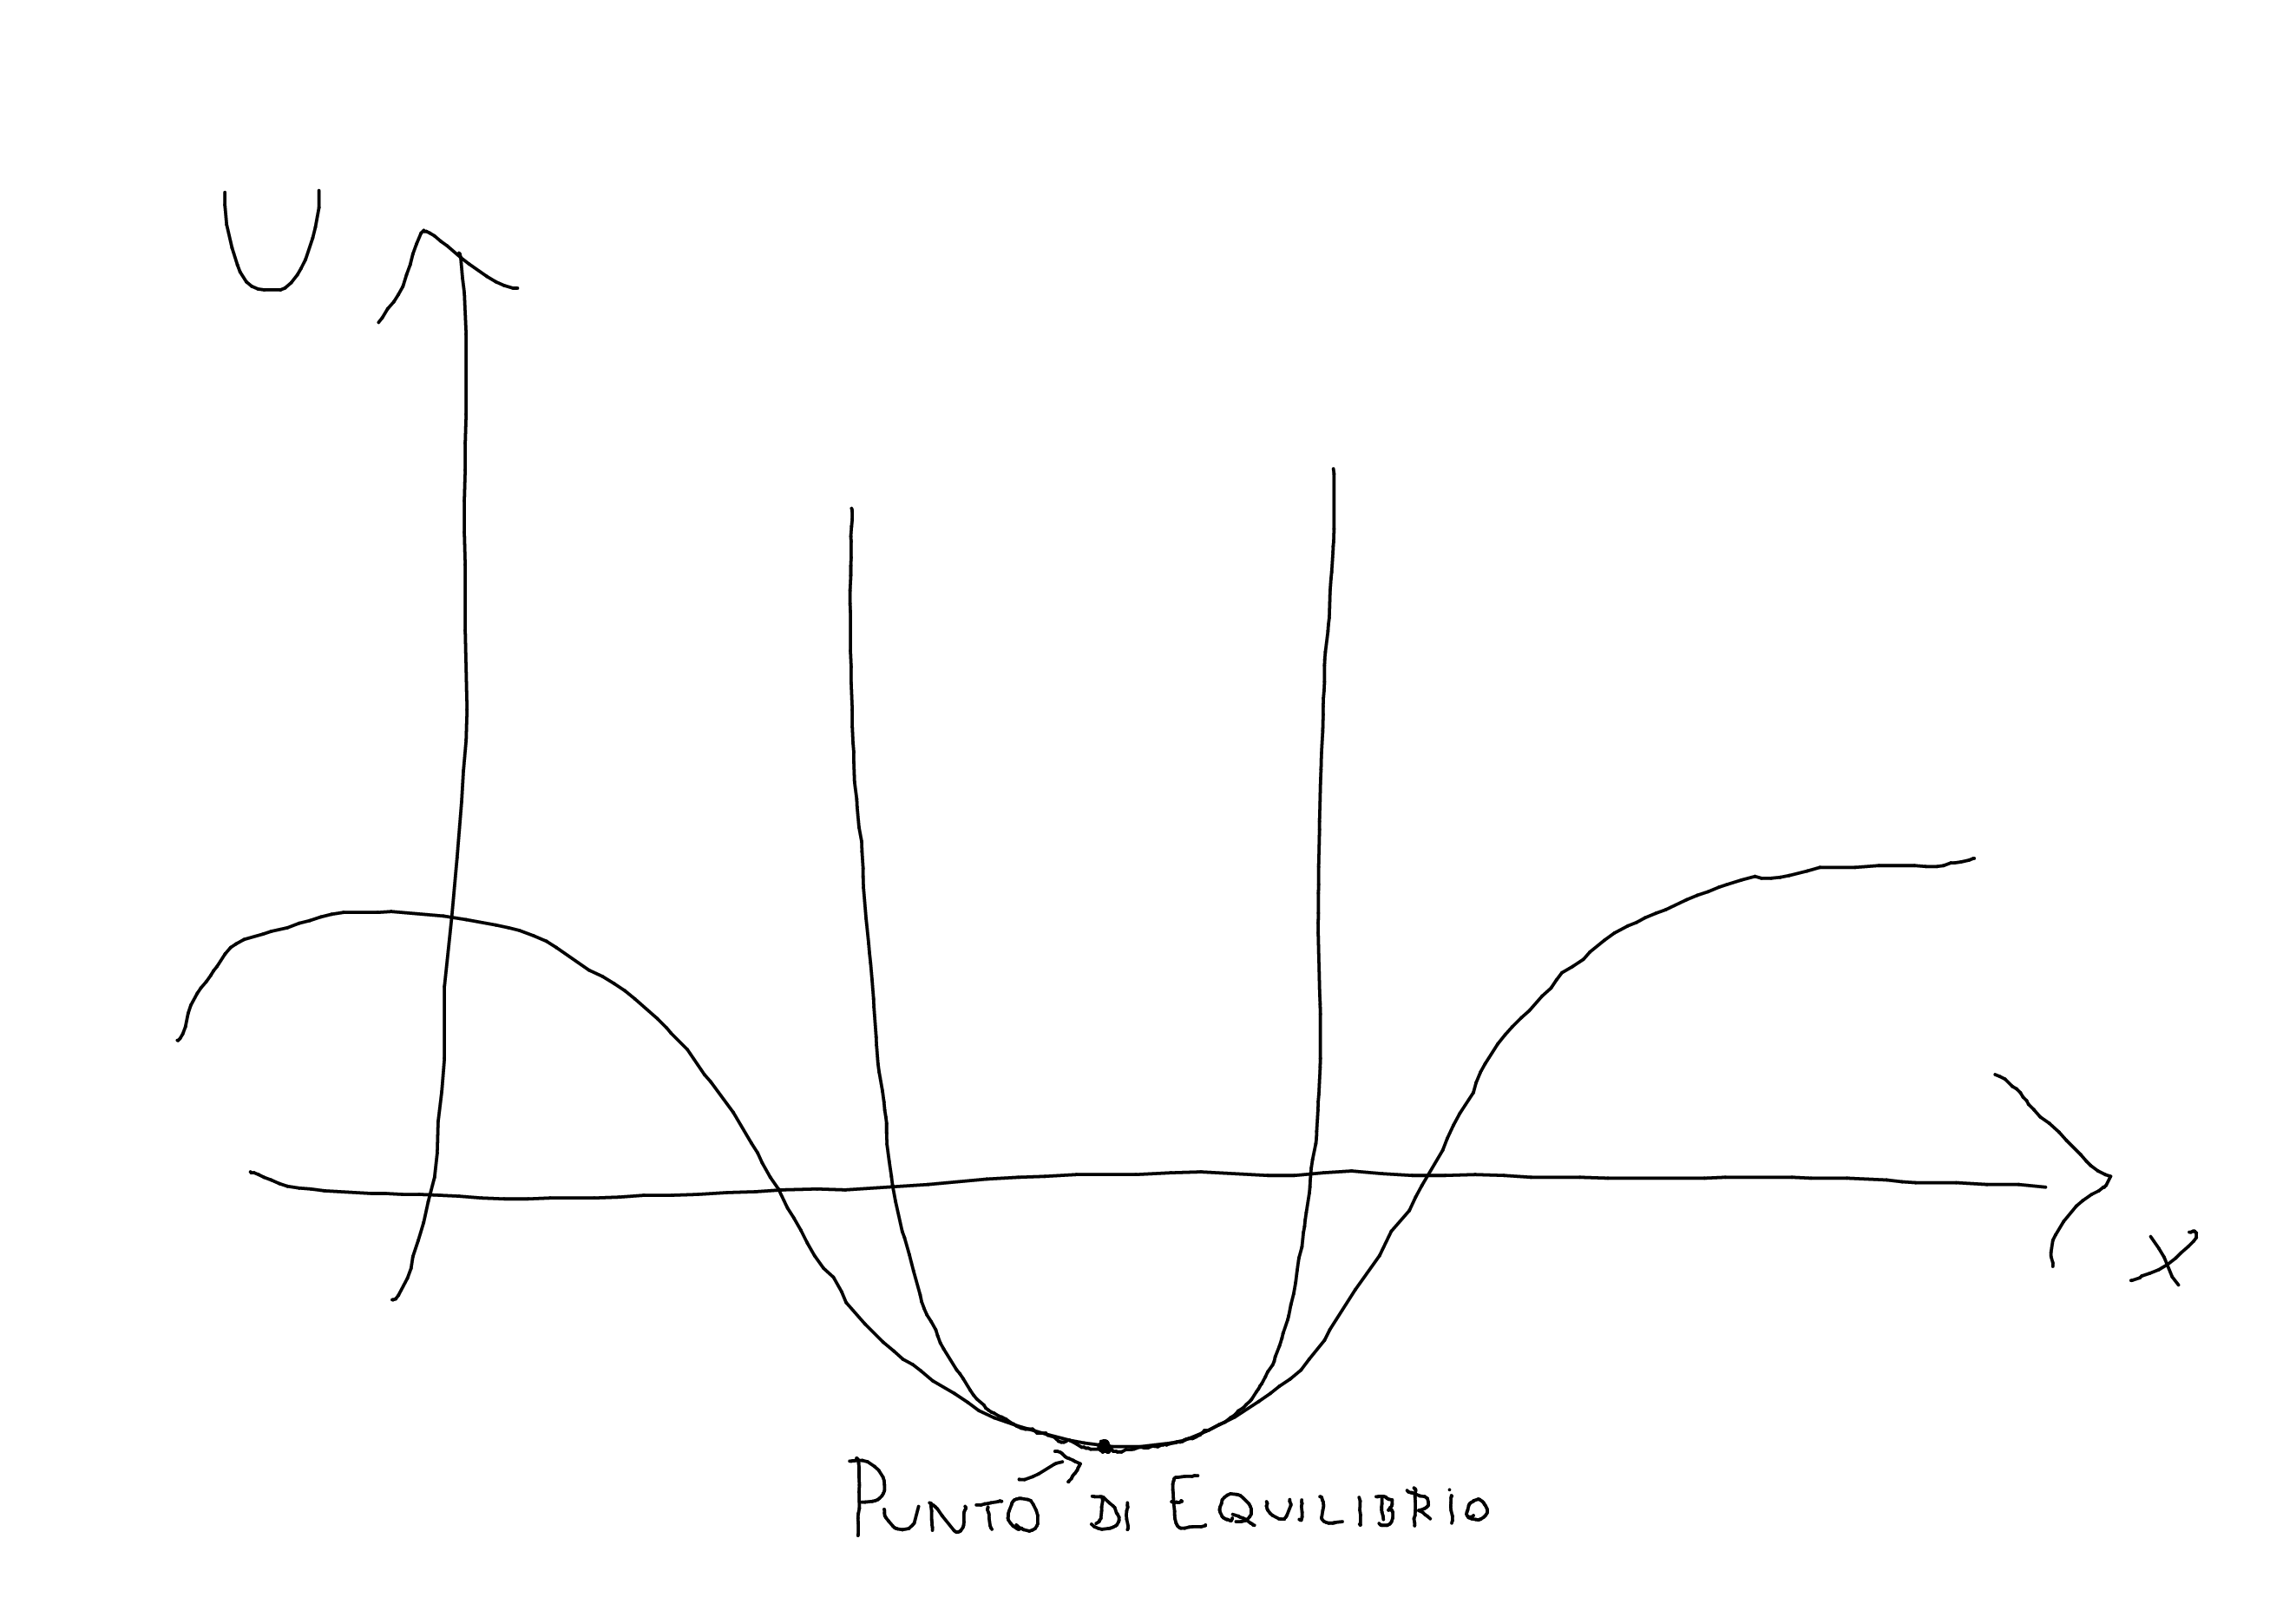
\includegraphics[width=0.5\textwidth]{EquilibrioEnergia.png}
\end{figure}
La scelta del punto di equilibrio dipende dai livelli di energia meccanica forniti al corpo, che permettono di raggiungere un punto di equilibrio o un altro similmente a quanto visto per la molla, in quanto per piccoli intorni possiamo approssimare una curva ad una parabola:
\begin{figure}[H]
    \centering
    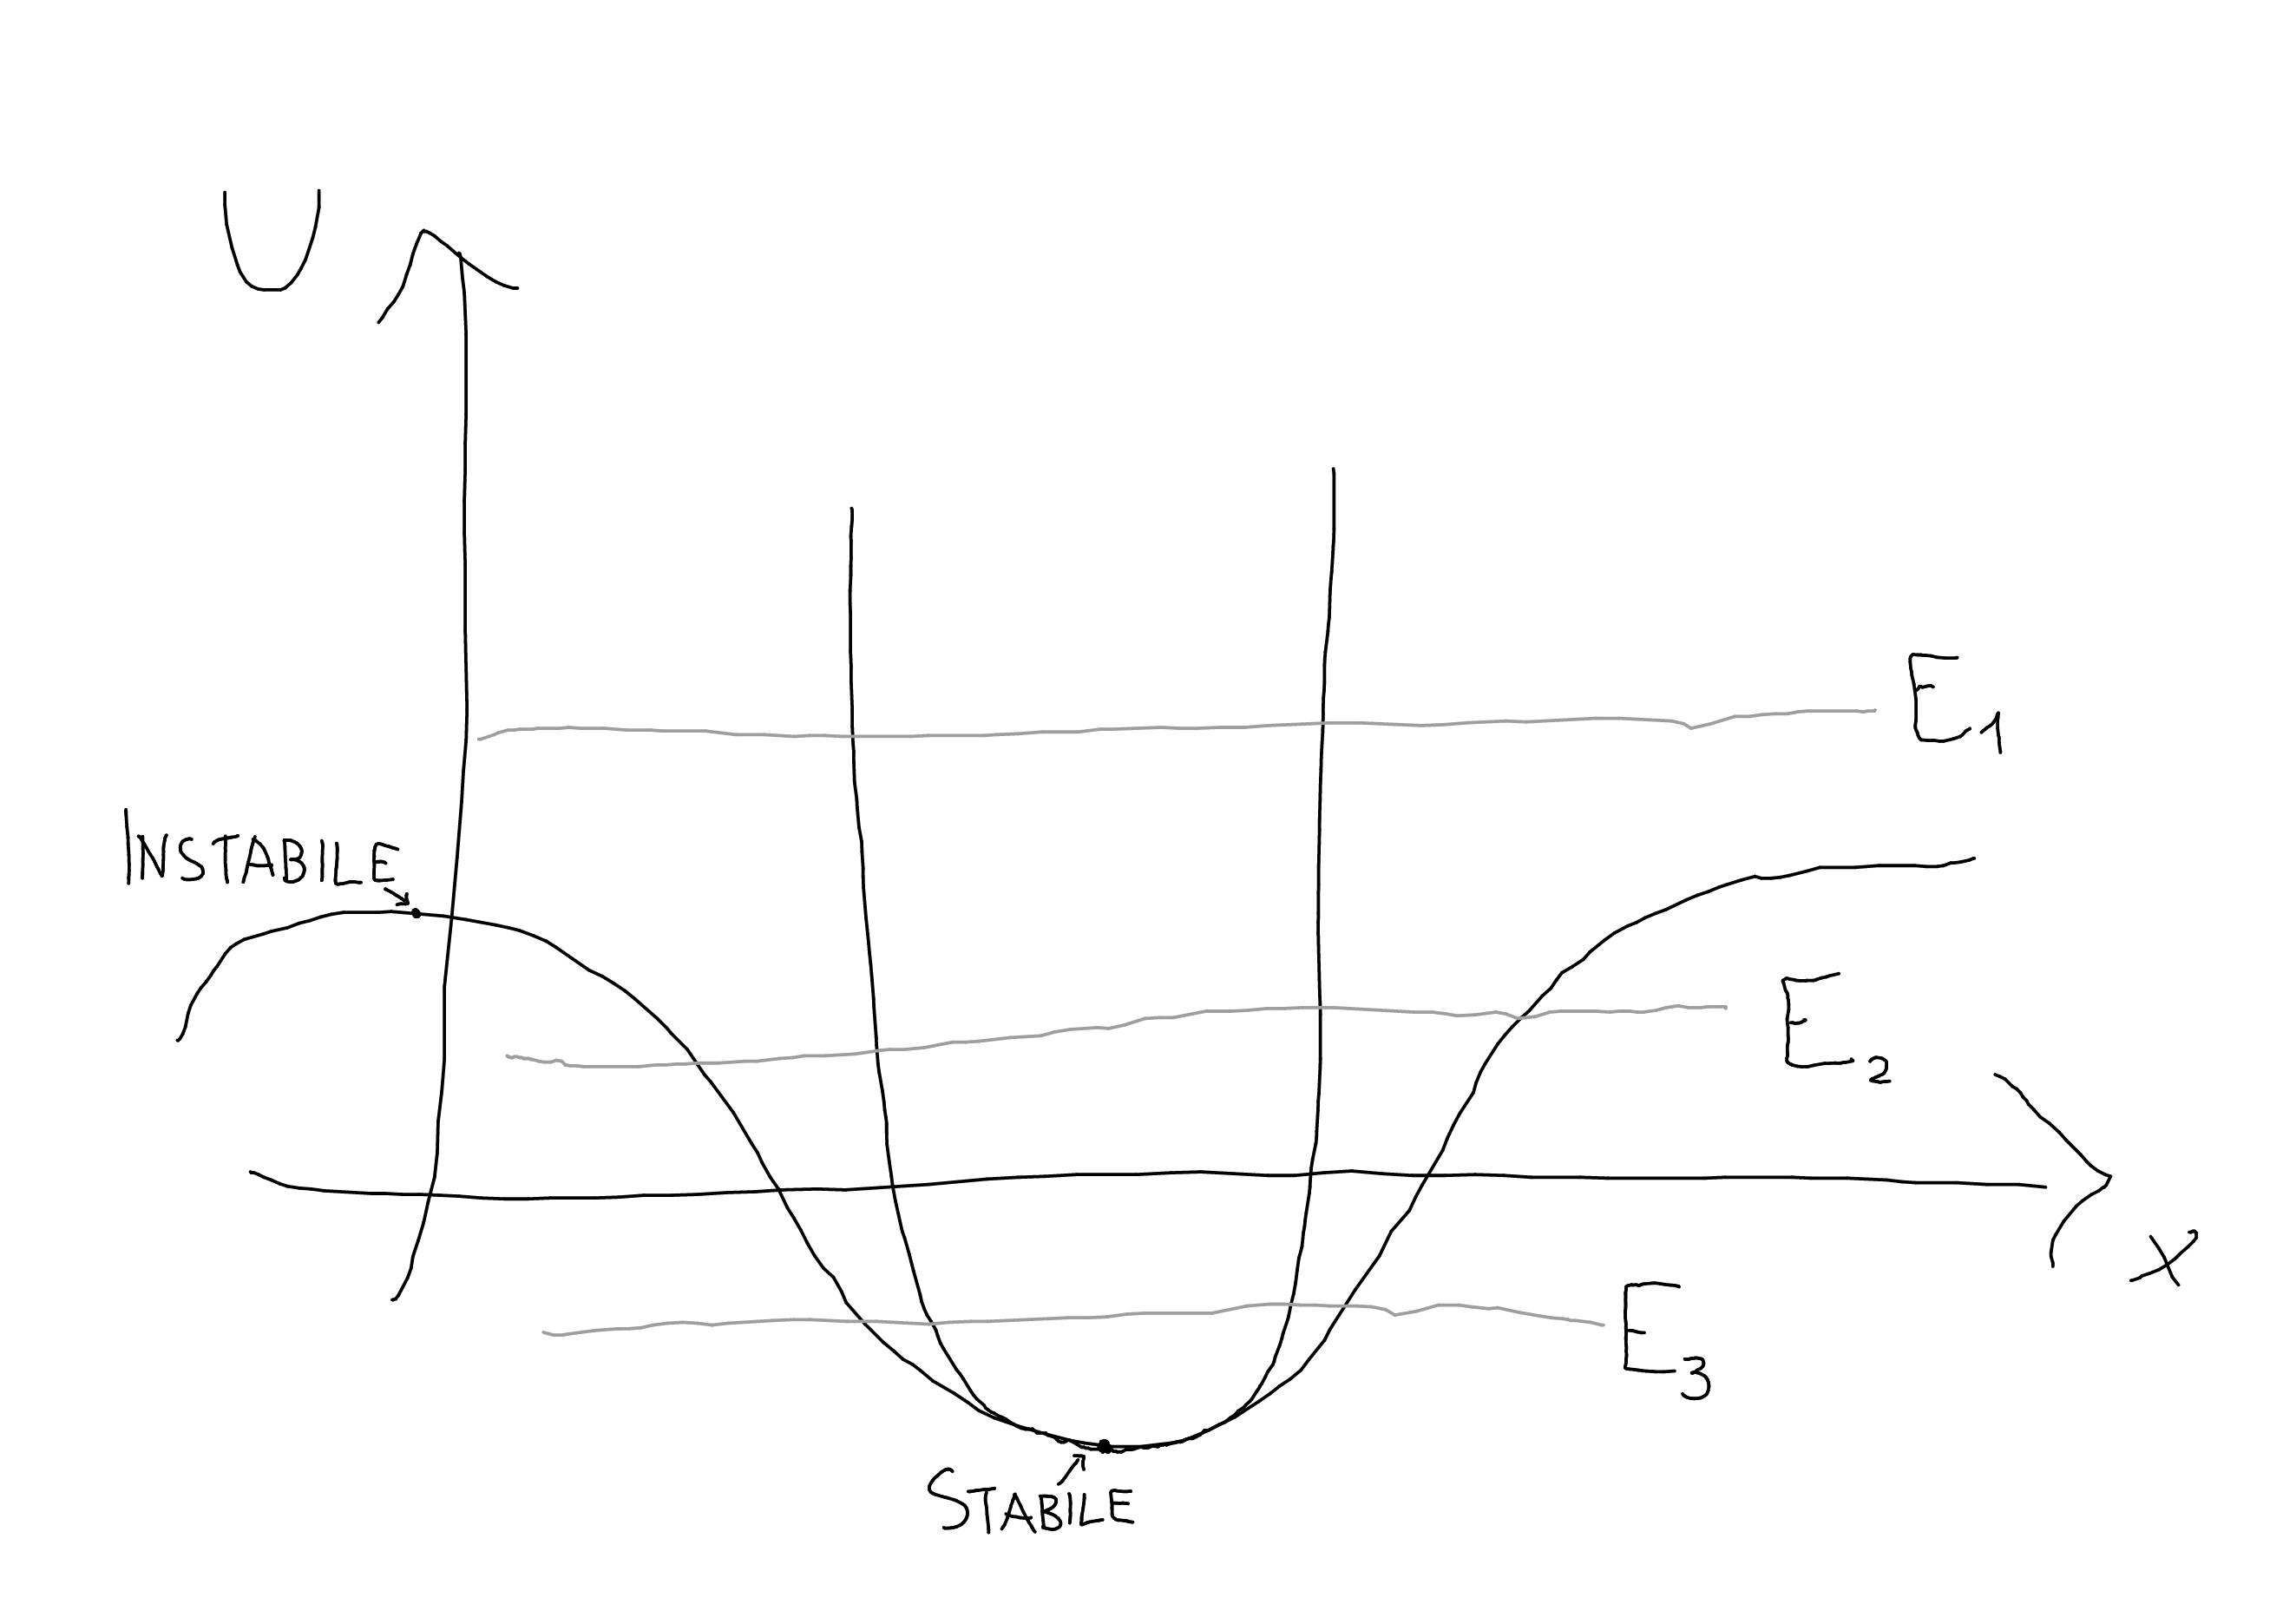
\includegraphics[width=0.5\textwidth]{EquilibriEnergiaMecc.png}
\end{figure}
Un equilibrio si dice \textbf{stabile} se perturbando il corpo, esso tende a riprendere l'equilibrio iniziale, mentre si dice \textbf{instabile} se tende ad allontanarsi. 
\paragraph{Esempi di Applicazioni dell'Energia}
L'energia fornisce numerosi strumenti per predire il comportamento di un corpo utilizzando velocità e posizioni, questo permette di non utilizzare le leggi orarie (e quindi conoscere esattamente istante per istante il moto del corpo) e limitarsi ad alcune informazioni relative a posizioni e velocità.\\
Ad esempio si può facilmente ricavare la posizione di massima altezza raggiunta da un proiettile lanciato con velocità obliqua:
\begin{align*}
    E_i=E_f\\
    \frac{1}{2}mv_0^2=\frac{1}{2}mv_0^2\cos^2\theta+mgh_M\\
    h_M=\frac{1}{2}\frac{m(v_0^2-v_0^2\cos^2\theta)}{mg}=\frac{v_0^2\sin^2\theta}{g}
\end{align*}
Che è propria la formula ottenuta utilizzando le leggi orarie.
\subparagraph{Pendolo Semplice}
Come per il proiettile utilizzare il Teorema Generale sull'Energia Meccanica permette di ottenere risultati senza passare per le leggi orarie, nel caso del pendolo, ciò ci permette di \textit{risolvere esattamente} l'equazione del moto, ricavando la velocità angolare in funzione dell'angolo e dell'ampiezza (consideriamo E come l'energia di un punto generico ed $E_0$ come l'energia al punto di altezza massima, cui corrisponde un angolo uguale all'ampiezza e dove la velocità e nulla):
\begin{align*}
    E=E_0\\
    \frac{1}{2}ml^2\Dot{\theta}^2+mgl(1-\cos\theta)=mgl(1-\cos\theta_0)\\
    \Dot{\theta}^2=2\frac{g}{l}(\cos\theta-\cos\theta_0)\\
    \boxed{\Dot{\theta}=\sqrt{2\frac{g}{l}(\cos\theta-\cos\theta_0)}}
\end{align*}
Osserviamo che la validità di questa relazione è limitata a $0\leq\theta\leq\pi$.\\
Infine notiamo che utilizzando lo sviluppo di Taylor $\cos\theta=1-\frac{\theta^2}{2}+o(\theta^4)\then 1-\cos\theta=\frac{\theta^2}{2}+o(\theta^4)$ possiamo esprimere come segue l'energia meccanica (anch'essa definita a meno di una costante):
\begin{equation}
\begin{split}
    E&=\frac{1}{2}mv^2+mgz=\\
    &=\frac{1}{2}ml^2\Dot{\theta}^2+mgl(1-\cos\theta)\approx\\
    &\approx\frac{1}{2}ml^2\Dot{\theta}^2+mg\frac{\theta^2}{2}=\\
    &=\boxed{\frac{1}{2}m(l^2\Dot{\theta}^2+g\theta^2)}
\end{split}
\end{equation}
\section{Momento Angolare e Momento di una Forza}
Si definisce \textbf{momento} di un vettore $\A$ associato alla posizione di un corpo rispetto a un certo \textbf{polo} O il seguente vettore:
\begin{equation}
    \M_O=\r\times\A
\end{equation}
Il momento della quantità di moto prende il nome di \textbf{momento angolare} e si definisce come segue:
\begin{equation}
    \l_{O}=\r\times\p=\r\times(m\v)
\end{equation}
Mentre il momento di una forza:
\begin{equation}
    \M_O=\r\times\F
\end{equation}
Si dimostra facilmente utilizzando il primo principio che la derivata temporale del momento angolare è il momento di una forza:
\begin{equation}
\begin{split}
    \dv{\l_O}{t}&=\dv{\r\times(m\v)}{t}=\\
    &=\dv{\r}{t}\times(m\v)+\r\times m\dv{\v}{t}=\\
    &=\v\times(m\v)+\r\times(m\a)=\\
    &=\r\times\F=\M_O
\end{split}
\end{equation}
\subsection{Campi di Forze Centrali}
Un campo di forze si definisce \textbf{centrale} se, dato un certo punto O, la direzione della forza è data sempre dalla direzione radiale del raggio vettore tra il punto O e un punto P dello spazio. Ossia possiamo scrivere:
\begin{equation}
    \boxed{\F(\r)=f(\abs{\r})\r}
\end{equation}
O alternativamente:
\[\F(\r)=f(\abs{\r})\vu{r}\]
Un esempio tipico è quello della forze gravitazionale:
\[\F(\r)=G\frac{mM}{\abs{\r}^2}\vu{r}\quad\quad f(\abs{\r})=G\frac{mM}{\abs{\r}^2}\]
Caratteristica peculiare dei campi centrali è la \textbf{conservazione del momento angolare} e dell'\textbf{energia meccanica}.
\paragraph{Conservazione del Momento Angolare}
Scegliendo come polo del momento di una forza il punto rispetto al quale una forza $\F$ è centrale otteniamo:
\[\M_O=\r\times\F=\r\times f(\abs{\r})\r=f(\abs{\r})(\r\times\r)=0=\dv{\l_O}{t}\iff\l_0=cost\]
\paragraph{Conservazione dell'Energia Meccanica}
Consideriamo la forza centrale di espressione $\F(\r)=f(\abs{\r})\r$ e notiamo che $\r\cdot\dif\r=r\dif r$. Possiamo notare ciò geometricamente osservando che:
\begin{figure}[H]
    \centering
    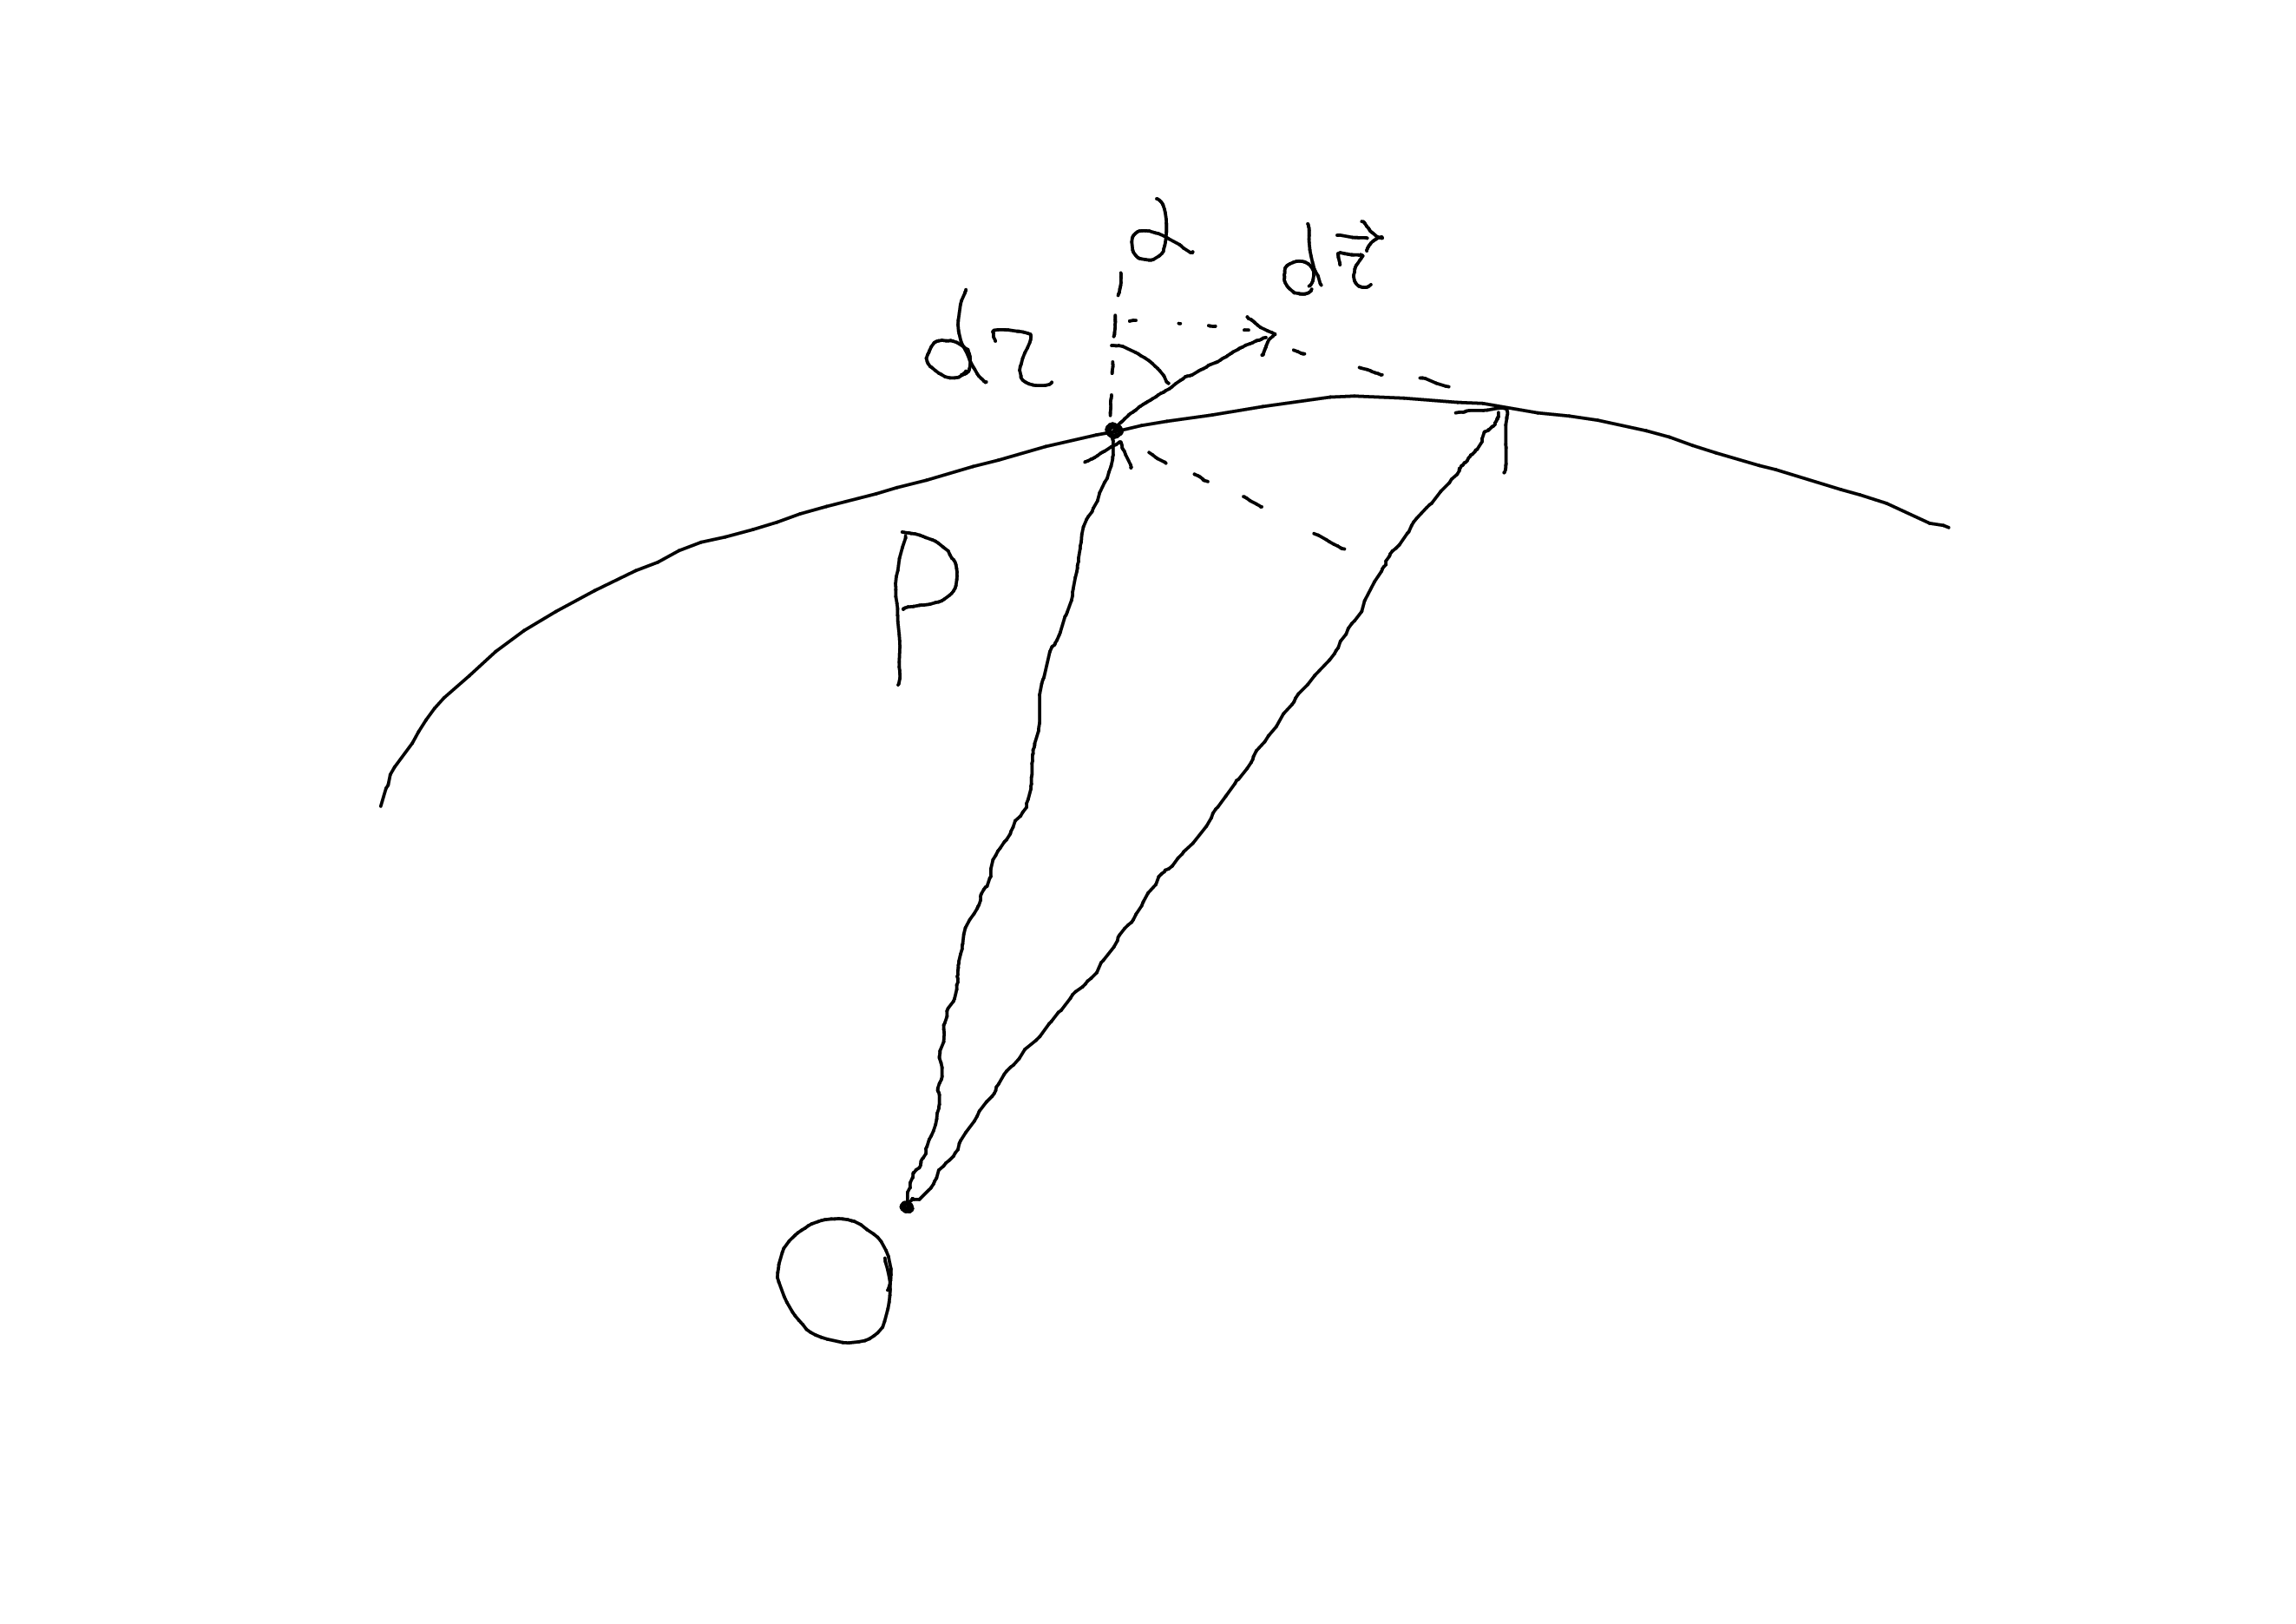
\includegraphics[width=0.5\textwidth]{EnergiaCampiCentrali.png}
\end{figure}
Da cui:
\[\r\cdot\dif\r=r\cos\alpha\abs{\dif\r}=r\dif r\]
Ossia la variazione del modulo della posizione corrsiponde alla proiezione dello spostamento parallelamente al vettore posizione.\\
Alternativamente notiamo analiticamente che:
\[\r\cdot\dif\r=x\dif x+y\dif y+z\dif z\quad\quad r=\sqrt{x^2+y^2+z^2}\]
E inoltre:
\begin{equation}
    \pdv{r}{x}=\frac{2x}{2\sqrt{x^2+y^2+z^2}}=\frac{x}{\sqrt{x^2+y^2+z^2}=\frac{x}{r}}
\end{equation}
Da cui:
\begin{equation}
\begin{cases}
    \pdv{r}{x}=\frac{x}{r}\\
    \pdv{r}{y}=\frac{y}{r}\\
    \pdv{r}{z}=\frac{z}{r}
\end{cases}
\end{equation}
Quindi esprimendo il differenziale esatto $\dif r$:
\begin{equation}
\begin{split}
    \dif r&=\pdv{r}{x}\dif x+\pdv{r}{y}\dif y+\pdv{r}{z}\dif z=\\
    &=\frac{x}{r}\dif x+\frac{x}{r}\dif z+\frac{z}{r}\dif z=\\
    &=\frac{x\dif x+y\dif y+z\dif z}{r}=\\
    &=\frac{\r\cdot\dif\r}{r}\iff \boxed{r\dif r=\r\dif\r}
\end{split}
\end{equation}
Pertanto ricaviamo che $\r\dif\r=r\dif r$ e calcolando il lavoro:
\[L=\int_{r_1}^{r_2}f(r)\r\dif\r=\int_{r_1}^{r_2}f(r) r\dif r=\int_{r_1}^{r_2}g(r)\dif r=G(r_2)-G(r_1)=U(r_1)-U(r_2)\]
Ossia il campo centrale è conservativo e conserva l'energia meccanica, risulta inoltre:
\[\dv{U(r)}{r}=-rf(r)\]
\note Questi risultati sono equivalenti all'affermare che esiste una certa funzione scalare U tale che il suo gradiente sia uguale al campo vettoriale $\F$, ossia che $\F$ è un campo conservativo.
\subsection{La Gravitazione}
Ricordando che la forza gravitazionale è una forza centrale concludiamo che essa conserva il momento angolare e l'energia meccanica. Dalla conservazione del momento angolare ricaviamo due conclusioni, una relativa a verso e direzione e l'altra al modulo.\\
\paragraph{Prima Legge di Keplero}
Dalla prima osserviamo che se verso e direzione rimangono costanti allora anche il piano contenente $\r$ e $\v$ deve rimanere perpendicolare alla stessa retta, ossia è lo stesso. Ciò che implica che le orbite dei corpi soggetti solo alla forza gravitazionale sono planari. Limitandoci a quest'osservazione enunciamo quindi la prima legge di Keplero:
\begin{enunc}[Prima Legge di Keplero]
I pianeti percorrono orbite ellittiche intorno al Sole, il quale occupa uno dei due fuochi. 
\end{enunc}
\paragraph{Seconda Legge di Kepler}
Dalla conservazione del modulo ricaviamo invece l'espressione della \textbf{velocità areale}





\end{document}